\documentclass[twoside,twocolumn,9pt]{article}

\usepackage{extsizes}
\usepackage[super,sort&compress,comma]{natbib} 
\usepackage[version=3]{mhchem}
\usepackage[left=1.5cm, right=1.5cm, top=1.785cm, bottom=2.0cm]{geometry}
\usepackage{balance}
\usepackage{mathptmx}
\usepackage{sectsty}
\usepackage{graphicx} 
\usepackage{lastpage}
\usepackage[format=plain,justification=justified,singlelinecheck=false,font={stretch=1.125,small,sf},labelfont=bf,labelsep=space]{caption}
\usepackage{float}
\usepackage{fancyhdr}
\usepackage{fnpos}
\usepackage[english]{babel}
\addto{\captionsenglish}{%
  \renewcommand{\refname}{Notes and references}
}
\usepackage{array}
\usepackage{droidsans}
\usepackage{charter}
\usepackage[T1]{fontenc}
\usepackage[usenames,dvipsnames]{xcolor}
\usepackage{setspace}
\usepackage[compact]{titlesec}
\usepackage{hyperref}
%%%Please don't disable any packages in the preamble, as this may cause the template to display incorrectly.%%%


\usepackage{epstopdf}%This line makes .eps figures into .pdf - please comment out if not required.

\definecolor{cream}{RGB}{222,217,201}

%-----E R Bittner ADDONS---
\usepackage{tikz}

\usepackage[most]{tcolorbox}

\usetikzlibrary{
    arrows.meta,
    positioning,
    calc,
    decorations.pathreplacing,
    shapes.geometric
}


\usepackage[version=4]{mhchem}

\usepackage{physics}      % derivatives, bras/kets, etc.
\usepackage{bm}           % bold math
\usepackage{mathtools}    % extensions to amsmath

\newtcolorbox{geombox}{
  enhanced,
  colback=gray!10,
  colframe=black,
  boxrule=0.8pt,
  arc=2mm,
  left=2mm,
  right=2mm,
  top=1mm,
  bottom=1mm,
  fonttitle=\bfseries
}




\begin{document}

\pagestyle{fancy}
\thispagestyle{plain}
\fancypagestyle{plain}{
%%%HEADER%%%
\renewcommand{\headrulewidth}{0pt}
}
%%%END OF HEADER%%%

%%%PAGE SETUP - Please do not change any commands within this section%%%
\makeFNbottom
\makeatletter
\renewcommand\LARGE{\@setfontsize\LARGE{15pt}{17}}
\renewcommand\Large{\@setfontsize\Large{12pt}{14}}
\renewcommand\large{\@setfontsize\large{10pt}{12}}
\renewcommand\footnotesize{\@setfontsize\footnotesize{7pt}{10}}
\makeatother

\renewcommand{\thefootnote}{\fnsymbol{footnote}}
\renewcommand\footnoterule{\vspace*{1pt}% 
\color{cream}\hrule width 3.5in height 0.4pt \color{black}\vspace*{5pt}} 
\setcounter{secnumdepth}{5}

\makeatletter 
\renewcommand\@biblabel[1]{#1}            
\renewcommand\@makefntext[1]% 
{\noindent\makebox[0pt][r]{\@thefnmark\,}#1}
\makeatother 
\renewcommand{\figurename}{\small{Fig.}~}
\sectionfont{\sffamily\Large}
\subsectionfont{\normalsize}
\subsubsectionfont{\bf}
\setstretch{1.125} %In particular, please do not alter this line.
\setlength{\skip\footins}{0.8cm}
\setlength{\footnotesep}{0.25cm}
\setlength{\jot}{10pt}
\titlespacing*{\section}{0pt}{4pt}{4pt}
\titlespacing*{\subsection}{0pt}{15pt}{1pt}
%%%END OF PAGE SETUP%%%

%%%FOOTER%%%
\fancyfoot{}
\fancyfoot[LO,RE]{\vspace{-7.1pt}
\includegraphics[height=9pt]{head_foot/LF}}
\fancyfoot[CO]{\vspace{-7.1pt}\hspace{11.9cm}
\includegraphics{head_foot/RF}}
\fancyfoot[CE]{\vspace{-7.2pt}\hspace{-13.2cm}
\includegraphics{head_foot/RF}}
\fancyfoot[RO]{\footnotesize{\sffamily{1--\pageref{LastPage} ~\textbar  \hspace{2pt}\thepage}}}
\fancyfoot[LE]{\footnotesize{\sffamily{\thepage~\textbar\hspace{4.65cm} 1--\pageref{LastPage}}}}
\fancyhead{}
\renewcommand{\headrulewidth}{0pt} 
\renewcommand{\footrulewidth}{0pt}
\setlength{\arrayrulewidth}{1pt}
\setlength{\columnsep}{6.5mm}
\setlength\bibsep{1pt}
%%%END OF FOOTER%%%

%%%FIGURE SETUP - please do not change any commands within this section%%%
\makeatletter 
\newlength{\figrulesep} 
\setlength{\figrulesep}{0.5\textfloatsep} 

\newcommand{\topfigrule}{\vspace*{-1pt}% 
\noindent{\color{cream}\rule[-\figrulesep]{\columnwidth}{1.5pt}} }

\newcommand{\botfigrule}{\vspace*{-2pt}% 
\noindent{\color{cream}\rule[\figrulesep]{\columnwidth}{1.5pt}} }

\newcommand{\dblfigrule}{\vspace*{-1pt}% 
\noindent{\color{cream}\rule[-\figrulesep]{\textwidth}{1.5pt}} }

\makeatother
%%%END OF FIGURE SETUP%%%

%%%TITLE, AUTHORS AND ABSTRACT%%%
\twocolumn[
  \begin{@twocolumnfalse}
{
\includegraphics[height=30pt]{head_foot/PCCP}\hfill\raisebox{0pt}[0pt][0pt]{
\includegraphics[height=55pt]{head_foot/RSC_LOGO_CMYK}}\\[1ex]

\includegraphics[width=18.5cm]{head_foot/header_bar}}\par
\vspace{1em}
\sffamily
\begin{tabular}{m{4.5cm} p{13.5cm} }


\includegraphics{head_foot/DOI} & \noindent\LARGE{
\textbf{The Geometry of Response$^\dag$}
} \\%Article title goes here instead of the text "This is the title"
\vspace{0.3cm} & \vspace{0.3cm} \\
 & \noindent
 \large{
 Eric R. Bittner,$^{\ast}$\textit{$^{a}$} 
 Carlos Silva-Acu\~na,\textit{$^{b\ddag}$} 
 and a cast of thousands\textit{$^{a}$}}   \\%Author names go here instead of "Full name", etc.

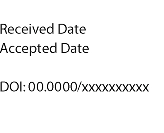
\includegraphics{head_foot/dates} & \noindent\normalsize{
Response functions occupy a central role throughout thermodynamics, statistical mechanics, and quantum dynamics, yet they are traditionally viewed as collections of susceptibilities describing how observables change under external perturbations. In this Perspective, we argue that response itself possesses an intrinsic differential geometry. Beginning with equilibrium thermodynamics, we show how symmetric response tensors define natural metrics while antisymmetric response components generate curvature two-forms that quantify nonreciprocal work and geometric transport. Extending these ideas to open quantum systems leads to a Liouvillian formulation in which environmental interactions induce connections, curvature, and holonomy on the manifold of dynamical generators. We demonstrate that nonlinear spectroscopy provides a natural experimental probe of this geometry by measuring the transport of Liouville-space pathways through an observable bundle. The canonical two-level system is reinterpreted as the universal local coordinate chart for this observational geometry, while a Duhamel expansion of the Liouvillian provides the differential calculus for systematically refining the local response manifold. Within this framework, model refinement is recast as geometric refinement, and spectroscopic analysis becomes an inverse problem of reconstructing local response geometry rather than merely fitting line shapes. Taken together, these developments establish a unified geometric framework connecting thermodynamics, open quantum dynamics, information geometry, and nonlinear spectroscopy, and suggest a broader program in which response geometry provides a common mathematical language for equilibrium and nonequilibrium physical phenomena.
} \\

\end{tabular}
 \end{@twocolumnfalse} \vspace{0.6cm}
  ]
%%%END OF TITLE, AUTHORS AND ABSTRACT%%%

%%%FONT SETUP - please do not change any commands within this section
\renewcommand*\rmdefault{bch}\normalfont\upshape
\rmfamily
\section*{}
\vspace{-1cm}


%%%FOOTNOTES%%%

\footnotetext{\textit{$^{a}$~University of Houston, Department of Physics, Houston, TX,  USA E-mail: ebittner@central.uh.edu}}
\footnotetext{\textit{$^{b}$~Address, Address, Town, Country. }}

\footnotetext{\dag~Additional footnotes to the title and authors can be included \textit{e.g.}\ `Present address:' or `These authors contributed equally to this work' as above using the symbols: \ddag, \textsection, and \P. Please place the appropriate symbol next to the author's name and include a \texttt{\textbackslash footnotetext} entry in the the correct place in the list.}


%%%END OF FOOTNOTES%%%

\section{Introduction}

Geometry has repeatedly emerged as a powerful organizing principle in physics. General relativity interprets gravitation through the curvature of spacetime, gauge theories describe interactions through connections on fiber bundles, and geometric phases reveal how global properties emerge from local evolution \cite{Einstein1915,Berry1984}. In each case, geometry provides more than a mathematical description; it identifies the fundamental structures governing physical response. A similar development has unfolded across thermodynamics and statistical physics. Over the past several decades, geometric ideas have appeared in equilibrium fluctuation theory, critical phenomena, stochastic thermodynamics, information geometry, synchronization, quantum thermodynamics, and open quantum systems \cite{Weinhold1975,Ruppeiner1979,Ruppeiner1995,Amari2000,Seifert2012}. Yet these developments have largely evolved in parallel, often employing different mathematical languages and emphasizing different physical applications. The extent to which they represent manifestations of a common underlying structure remains an open question.

The central thesis of this review is that the recurring appearance of geometry throughout thermodynamics is not accidental. Rather, geometry emerges because thermodynamics is fundamentally a theory of response. Thermodynamic systems are characterized not only by their states but by how those states respond to perturbations, constraints, environmental interactions, and observations. From this perspective, geometry is not a property of thermodynamic states alone; it is a property of how those states respond. The various geometric structures that appear throughout thermodynamics—metrics, connections, curvature, and holonomy—arise as different manifestations of this underlying response geometry.

The earliest examples of thermodynamic geometry arose in equilibrium statistical mechanics. Building upon Einstein’s theory of fluctuations, Weinhold and Ruppeiner demonstrated that thermodynamic response functions naturally define metric structures on spaces of equilibrium states \cite{Einstein1910,Weinhold1975,Ruppeiner1979,Ruppeiner1995}. These metrics encode susceptibilities, stability, and critical behavior through local notions of distance and curvature. Near critical points, diverging fluctuations induce singular geometric structures whose properties reflect the growth of correlations and the breakdown of characteristic length scales \cite{Ruppeiner1995,Gu2010}. Information geometry provides a closely related perspective in which distinguishability between neighboring probability distributions is quantified through the Fisher information metric and its quantum generalizations \cite{Fisher1925,Amari2000,BraunsteinCaves1994,Paris2009}. Together, these approaches establish a geometric interpretation of fluctuations, stability, and statistical distinguishability.

The geometric character of thermodynamics becomes even more pronounced away from equilibrium. The development of stochastic thermodynamics elevated fluctuating trajectories to fundamental objects and established exact relationships connecting work, entropy production, and irreversibility \cite{Jarzynski1997,Crooks1999,Seifert2012}. Within this framework, geometric phases and pumping phenomena emerge naturally when systems are driven through cyclic variations of control parameters \cite{Sinitsyn2007,Sinitsyn2009}. Excess work, excess entropy production, and nonequilibrium transport acquire geometric interpretations closely analogous to Berry phases in quantum mechanics. These developments suggest that geometry is not merely associated with equilibrium state spaces but is a more general property of thermodynamic response itself.

A complementary line of development concerns synchronization and collective dynamics in driven and dissipative systems. Beginning with the observations of Huygens and extending through the modern theory of coupled oscillators, synchronization provides a paradigmatic example of emergent order arising from interactions among many dynamical degrees of freedom \cite{Kuramoto1984,Strogatz2003}. More recently, synchronization has been extended to quantum systems, where common environments and correlated dissipation can generate phase locking, collective oscillations, and enhanced coherence \cite{Mari2013,Giorgi2013,Bittner2024Sync,Bittner2025JCP}. These studies challenge the traditional view of dissipation as a purely destructive process and instead reveal its capacity to generate organization and collective structure. From a geometric perspective, synchronization may be viewed as the emergence of effective dynamical manifolds and collective coordinates that constrain and organize system response. In this sense, synchronization provides a bridge between nonequilibrium dynamics and response geometry.

Parallel developments in quantum information theory have further expanded the geometric viewpoint. Quantum Fisher information, Bures metrics, and thermodynamic length provide geometric measures of sensitivity, distinguishability, and dissipation in quantum systems \cite{Uhlmann1976,BraunsteinCaves1994,Zanardi2007,Gu2010,Paris2009}. These constructions have become central tools for characterizing quantum phase transitions, parameter estimation, and quantum thermodynamic processes. More generally, they reinforce the idea that response, rather than state alone, provides the natural foundation for geometric descriptions of physical systems.

Open quantum systems provide a particularly rich setting in which these themes converge. Environmental interactions generate decoherence, relaxation, synchronization, collective behavior, and nonequilibrium steady states while simultaneously producing new forms of response unavailable in isolated systems. Recent work has demonstrated that open quantum systems may support geometric structures including work one-forms, curvature two-forms, geometric phases, and holonomies defined on manifolds of control parameters \cite{SivakCrooks2012,NESSGeometry2019,GeometricThermoOQS2026}. At the same time, dissipative phase transitions and Liouvillian criticality reveal striking analogies between nonequilibrium steady states and equilibrium critical phenomena \cite{Prosen2010,DissipativeCriticality2025}. These results suggest that nonequilibrium response possesses a geometric structure that extends, and in some cases transcends, traditional equilibrium formulations.

Taken together, these developments point toward a broader unifying picture. Much of the existing literature has focused on geometric structures associated with states and probability distributions. Metrics derived from thermodynamic potentials, entropy functions, or statistical distinguishability characterize fluctuations, susceptibilities, and stability. Yet nonequilibrium systems reveal an additional geometric sector associated with circulation, transport, and cyclic response. Work performed around thermodynamic cycles, geometric pumping, excess entropy production, and nonequilibrium transport all depend upon path-dependent response rather than state properties alone.

We therefore propose that a complete thermodynamic geometry contains both a symmetric metric sector and an antisymmetric curvature sector. The symmetric sector encodes fluctuations, susceptibilities, stability, and distinguishability. The antisymmetric sector encodes circulation, transport, irreversibility, cyclic work, and geometric phase accumulation. From this perspective, the distinction between fluctuations, transport, work, and information reflects different projections of a common response geometry. Metrics characterize what nearby states can be distinguished; curvature characterizes how response accumulates as systems are transported through parameter space.

The goal of this review is to synthesize these developments and explore the consequences of this viewpoint. We argue that geometry is not a property of thermodynamic states alone but of how those states respond. This perspective provides a common framework linking equilibrium fluctuations, critical phenomena, stochastic thermodynamics, synchronization, information geometry, open quantum systems, and observational descriptions. Throughout, our aim is not merely to survey existing results but to identify the common principles that may underlie a unified geometric theory of thermodynamic response.

\subsection{Historical Development of Thermodynamic Geometry}

The relationship between geometry and thermodynamics has a long and complex history. Although modern discussions often focus on geometric metrics or information-theoretic constructions, many of the underlying ideas can be traced to the earliest formulations of thermodynamics itself. Concepts such as state space, equilibrium manifolds, cyclic processes, and integrability conditions are geometric in character, even when not explicitly expressed in the language of differential geometry.

In classical thermodynamics, the geometric viewpoint emerged naturally through the work of Gibbs and Carathéodory. Equilibrium states were represented as points on thermodynamic manifolds, while thermodynamic processes corresponded to trajectories connecting neighboring states. The existence of thermodynamic potentials and Maxwell relations reflected underlying integrability conditions, and the work performed during cyclic processes was associated with areas enclosed in thermodynamic state spaces. These constructions established a geometric foundation for thermodynamics long before the development of modern thermodynamic geometry.

A more explicit geometric formulation emerged through fluctuation theory. Einstein’s theory of thermodynamic fluctuations revealed a close connection between probability distributions and local response functions, suggesting that fluctuations define a natural notion of distance between neighboring equilibrium states. Building on these ideas, Weinhold introduced a metric structure derived from the Hessian of the internal energy, while Ruppeiner developed an entropy-based metric directly related to fluctuation probabilities. These approaches demonstrated that thermodynamic susceptibilities define local geometric structures whose properties encode stability, correlations, and critical behavior. Over subsequent decades, thermodynamic metrics were applied extensively to fluids, magnetic systems, black-hole thermodynamics, and critical phenomena, establishing metric geometry as one of the central themes of modern thermodynamics.

A second major development arose from information theory and statistical inference. Fisher’s information metric provided a measure of distinguishability between neighboring probability distributions and established a geometric framework for statistical estimation. The subsequent development of information geometry extended these ideas to broad classes of statistical models, while quantum generalizations led to the Bures metric, quantum Fisher information, and related measures of quantum distinguishability. These constructions linked geometry, information, and thermodynamics through a common notion of statistical response, revealing deep connections between fluctuations, inference, and sensitivity to external perturbations.

The scope of thermodynamic geometry expanded dramatically with the development of nonequilibrium statistical mechanics and stochastic thermodynamics. In these frameworks, fluctuating trajectories rather than equilibrium states become the fundamental objects of description. Fluctuation theorems, entropy production, and nonequilibrium work relations revealed new forms of thermodynamic structure that depend explicitly on paths through parameter space. Geometric phases, pumping phenomena, and excess thermodynamic quantities emerged as natural consequences of cyclic driving, introducing geometric concepts closely analogous to Berry phases and gauge fields into nonequilibrium thermodynamics. These developments suggested that thermodynamic geometry extends beyond metrics on state spaces and includes path-dependent structures associated with transport and irreversibility.

At the same time, studies of synchronization and collective dynamics revealed another route by which geometry enters thermodynamics. Classical and quantum synchronization demonstrate how interactions and environmental couplings can generate collective coordinates, reduced manifolds, and emergent dynamical organization. These phenomena suggest that geometry may arise not only from the structure of equilibrium states but also from the mechanisms that organize dynamical response. In this sense, synchronization provides a bridge between nonequilibrium dynamics and geometric descriptions of collective behavior.

More recently, geometric approaches have been developed for open quantum systems and nonequilibrium steady states. Dissipative phase transitions, Liouvillian criticality, geometric pumping, and steady-state response have revealed structures involving connections, curvature, and holonomy that have no direct equilibrium analog. These developments indicate that the geometric description of thermodynamics must ultimately encompass both equilibrium and nonequilibrium phenomena, as well as both classical and quantum systems.

Viewed from this historical perspective, thermodynamic geometry has evolved through a sequence of increasingly general frameworks. The earliest formulations emphasized state spaces and integrability. Fluctuation theory introduced metric structures associated with response and stability. Information geometry generalized these ideas to statistical distinguishability. Nonequilibrium thermodynamics introduced path-dependent geometric phases and transport phenomena. Synchronization and collective dynamics revealed the emergence of geometric organization through dissipation. Open quantum systems extended these concepts to steady-state manifolds exhibiting curvature and holonomy.

The central theme emerging from this progression is that geometry appears whenever thermodynamic response is examined at a sufficiently fundamental level. The historical development of thermodynamic geometry may therefore be viewed not as a succession of unrelated constructions but as a gradual expansion of the notion of response itself—from equilibrium states, to fluctuations, to trajectories, to collective dynamics, and ultimately to observable-dependent descriptions. This broader perspective motivates the central thesis of the present review: geometry is not a property of thermodynamic states alone but of how those states respond.


\begin{figure*}[t]
\centering
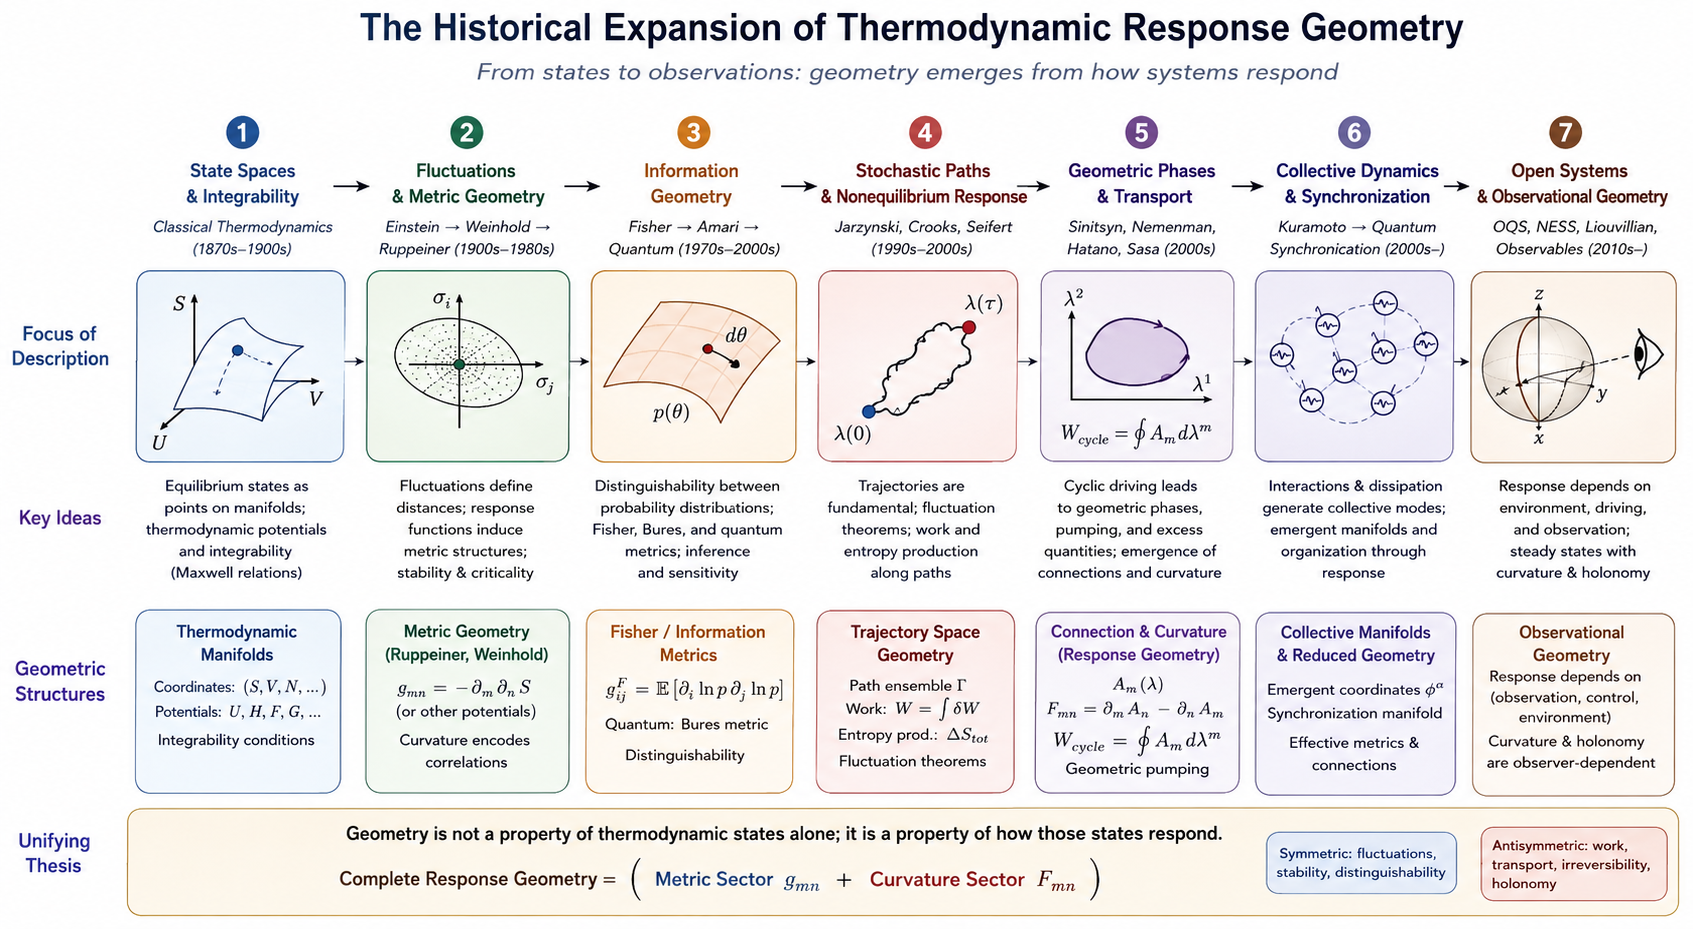
\includegraphics[width=\textwidth]{Figures/2F7A6768-CD89-4332-9FC2-827ED817DBA7.png}
\caption{
Conceptual progression of the response-geometry program.
(\textbf{a}) Classical thermodynamics, where response is encoded by
equilibrium fluctuations and susceptibilities, giving rise to
geometric structures such as metrics, curvature, and cycle
holonomies on the thermodynamic state manifold.
(\textbf{b}) Open quantum systems, where environmental interactions
generate nonequilibrium steady states and induce geometric
response through coherence, dissipation, and basis
misalignment between energy and pointer representations.
(\textbf{c}) Observable-conditioned thermodynamics, in which the
geometry depends explicitly on the observational frame,
leading to gauge-like structures associated with restricted
access to system information.
(\textbf{d}) Spectroscopic reconstruction, where geometric quantities
are inferred from experimentally accessible observables,
including nonlinear optical response, intensity borrowing,
and bright–dark state mixing. In this picture, curvature,
connections, and holonomy emerge as measurable properties
of response rather than purely abstract mathematical
constructions. The overall program seeks to establish a
unified geometric description of thermodynamic response
across equilibrium, nonequilibrium, and quantum regimes.
}
\label{fig:program_cartoon}
\end{figure*}


\section{Metrics, Connections, Curvature, and Response}

Geometric descriptions of physical systems generally arise
from four closely related structures: a metric, a connection,
a curvature, and the corresponding response functions that
render these quantities observable. Although these objects
appear in diverse contexts ranging from general relativity
to gauge theory and information geometry, they share a
common interpretation as measures of how a system changes
under variation of external parameters.

The most familiar geometric object is the metric tensor.
A metric defines a local notion of distance on a manifold and
thereby quantifies distinguishability between neighboring
states. In thermodynamics, the Weinhold and Ruppeiner
metrics relate this notion of distance to susceptibilities and
equilibrium fluctuations. In quantum mechanics, analogous
structures arise through the quantum geometric tensor,
Bures metric, and quantum Fisher information, which
measure the sensitivity of quantum states to parameter
variation. In each case, the metric characterizes the local
response of the system and provides a geometric measure of
its fluctuations.

A metric alone, however, does not determine how local
information is compared across different points of a manifold.
This role is played by a connection. A connection specifies
how vectors, operators, or states are transported between
neighboring points and therefore encodes the choice of local
reference frame. Familiar examples include the Levi-Civita
connection of differential geometry, Berry connections in
quantum mechanics, and gauge connections in field theory.
Physically, connections determine how response measured at
one point is related to response measured at another.

Curvature quantifies the extent to which parallel transport
depends on path. Equivalently, it measures the failure of
successive parameter variations to commute. In differential
geometry, curvature governs the holonomy acquired by a
vector transported around a closed loop. In gauge theories,
it corresponds to the field strength tensor. In quantum
mechanics, Berry curvature determines geometric phases
accumulated under cyclic evolution. More generally,
curvature provides a local measure of nonintegrability:
whenever response depends on the order in which control
parameters are varied, a nonzero curvature is present.

The geometric structures introduced above become physically
meaningful only through response. Metrics are inferred from
fluctuations and susceptibilities, connections from the
transport of local reference frames, and curvature from
cyclic response and holonomy. From this perspective,
geometry is not an abstract property imposed upon a
physical system but rather an emergent description of how
the system responds to external perturbations.

The central premise of the present work is that response
itself may be regarded as a geometric object. Observable
changes induced by parameter variation define local frames
on a control manifold, while the incompatibility of distinct
response channels generates connections and curvature.
This viewpoint naturally unifies equilibrium fluctuation
geometry, nonequilibrium thermodynamic response, and
the geometric structures that arise in open quantum
systems.

\subsection{Scope and Organization of This Review}

The literature connecting geometry and thermodynamics has grown rapidly over the past several decades and now spans diverse areas including equilibrium fluctuation theory, information geometry, stochastic thermodynamics, quantum thermodynamics, nonequilibrium statistical mechanics, synchronization, and open quantum systems. A comprehensive review of all geometric approaches is therefore beyond the scope of a single article. Instead, our objective is to identify the common principles that underlie these developments and to examine them through the unifying concept of response geometry.

Our emphasis is consequently not on providing an exhaustive catalog of geometric constructions, but rather on understanding why geometric structures repeatedly emerge in thermodynamic descriptions. Throughout the review, we focus on the relationship between physical response and geometry, emphasizing how fluctuations, susceptibilities, transport coefficients, entropy production, synchronization, and work may all be interpreted as manifestations of a common geometric framework. Particular attention is devoted to the distinction between metric structures associated with fluctuations and distinguishability, and curvature structures associated with circulation, transport, and cyclic response.

The perspective adopted here naturally spans both classical and quantum systems. We begin with equilibrium thermodynamics, where geometric concepts arise through fluctuations, susceptibilities, and critical phenomena. We then consider stochastic thermodynamics and nonequilibrium response, where geometric phases and excess thermodynamic quantities emerge from trajectory-dependent dynamics. Synchronization and collective behavior are subsequently discussed as examples of geometric organization induced by interactions and dissipation. We then turn to information geometry and open quantum systems, where notions of distinguishability, coherence, and steady-state response reveal increasingly rich geometric structures.

The final sections explore recent developments in observable-dependent thermodynamics and observational geometry. These approaches suggest that geometric structure may depend not only on the underlying dynamics but also on the observational framework through which a system is described. Such ideas point toward a broader conception of thermodynamic geometry in which states, trajectories, controls, environments, and observations all contribute to the geometric characterization of response.

A recurring theme throughout this review is that a complete geometric description of thermodynamics requires both a symmetric and an antisymmetric sector. The symmetric sector, represented by metric structures, characterizes fluctuations, susceptibilities, stability, and distinguishability. The antisymmetric sector, represented by connections and curvature, characterizes circulation, transport, irreversibility, and work. While these structures often appear under different names in different communities, we argue that they are most naturally understood as complementary components of a unified response geometry.



\section{Classical Thermodynamic Geometry}\label{sec:classical}

Before the introduction of statistical mechanics or differential geometry, thermodynamics arose from an intensely practical problem: understanding the operation and limitations of heat engines. The industrial revolution transformed steam power into one of the dominant technologies of the nineteenth century, motivating fundamental questions concerning the conversion of heat into mechanical work. Carnot’s analysis of reversible cycles, later reformulated by Clausius, Kelvin, and Gibbs, established thermodynamics as a quantitative theory of energy transformation, efficiency, and response.

From a modern perspective, it is striking that many of the central concepts of thermodynamics emerged not from the study of equilibrium states themselves but from the study of transformations between states. Heat capacities, compressibilities, expansion coefficients, and engine efficiencies all characterize how a system responds to changes in its environment. Long before the introduction of thermodynamic manifolds and geometric formalisms, thermodynamics was therefore fundamentally concerned with response.

This perspective remains relevant today. While steam engines motivated the original development of thermodynamics, modern information technologies are similarly constrained by thermodynamic principles. The energetic cost of computation, information processing, communication, and quantum control all depend upon the response of physical systems to external driving. Concepts such as entropy production, thermodynamic length, and information geometry have consequently become increasingly important in fields ranging from machine learning and nanoscale devices to quantum technologies. In this sense, thermodynamics continues to serve as an organizing principle for successive technological revolutions, linking the steam engines of the Industrial Age to the information-processing systems of the twenty-first century.

\subsection{Thermodynamic State Spaces}

Classical thermodynamics is fundamentally a theory of states and transformations between them. The equilibrium condition of a macroscopic system may be specified by a set of extensive variables
\begin{align}
X^a=(S,V,N_1,N_2,\ldots),
\end{align}
which define points on a thermodynamic manifold. The fundamental relation
\begin{align}
U = U(S,V,N_1,N_2,\ldots)
\end{align}
then determines the equilibrium properties of the system and provides a complete thermodynamic description. In this sense, thermodynamics may be viewed as the study of a differentiable manifold embedded within a higher-dimensional space of thermodynamic variables.

The differential structure of this manifold is encoded in the First Law,
\begin{align}
dU = T\,dS - P\,dV + \sum_i \mu_i\, dN_i,
\end{align}
which defines the conjugate intensive variables through
\begin{align}
T=\left(\frac{\partial U}{\partial S}\right){V,N},
\qquad
P=-\left(\frac{\partial U}{\partial V}\right){S,N},
\qquad
\mu_i=\left(\frac{\partial U}{\partial N_i}\right)_{S,V}.
\end{align}
The intensive variables therefore arise naturally as components of the gradient of the thermodynamic potential. Geometrically, they determine the local tangent structure of the equilibrium manifold and characterize the response of the system to infinitesimal changes in its state variables.

This viewpoint was formalized by Gibbs and later generalized by Carathéodory through the introduction of thermodynamic surfaces and Pfaffian forms. Modern geometric treatments often regard the equilibrium manifold as a Legendre submanifold embedded within a higher-dimensional contact space whose coordinates are given by
\begin{align}
(U,S,V,N_i,T,-P,\mu_i).
\end{align}
Within this framework, the First Law appears as a contact one-form whose vanishing defines the equilibrium manifold. Legendre transformations correspond to changes of thermodynamic representation, while the physical content of thermodynamics remains invariant under such transformations.

While these geometric constructions provide an elegant mathematical formulation of equilibrium thermodynamics, their physical significance lies in the relationships among neighboring states. Thermodynamic observables are rarely determined by a state alone; rather, they are inferred from how the system responds to perturbations. Temperature, pressure, compressibility, heat capacity, and susceptibility all characterize changes induced by variations of external constraints. Consequently, the geometry of thermodynamics is fundamentally tied not only to the structure of state space but also to the response connecting nearby states.

This observation motivates a shift in perspective. Rather than viewing the thermodynamic manifold as a static collection of equilibrium states, one may regard it as the arena on which response is defined. From this standpoint, geometry emerges through the differential relations connecting neighboring states, and the central objects of interest become the response functions that characterize these relations. These response functions form the bridge between thermodynamic state spaces and the geometric structures developed throughout the remainder of this review.


\subsection{Response Functions and Susceptibility Matrices}


The local geometry of a thermodynamic manifold is determined by how a system responds to perturbations. In equilibrium thermodynamics, this information is encoded in the derivatives of the thermodynamic potentials and is quantified experimentally through response functions such as heat capacities, compressibilities, expansion coefficients, and magnetic susceptibilities. These quantities characterize the sensitivity of a system to changes in external constraints and provide the first indication that thermodynamic response possesses an intrinsic geometric structure.

For a simple one-component fluid described by the fundamental relation
\begin{align}
U=U(S,V),
\end{align}
the differential response is determined by the Hessian matrix
\begin{align}
K_{ij}
=
\frac{\partial^2 U}
{\partial X_i \partial X_j}
=
\begin{pmatrix}
U_{SS} & U_{SV}\\
U_{SV} & U_{VV}
\end{pmatrix},
\end{align}
where $X=(S,V)$. The diagonal elements characterize the response of the system to changes in entropy and volume individually, while the off-diagonal element \(U_{SV}\) describes the coupling between thermal and mechanical degrees of freedom.

The Hessian matrix plays a role analogous to a stiffness tensor in elasticity theory. Through the First Law, variations of the conjugate intensive variables may be expressed as
\begin{align}
\begin{pmatrix}
dT\\
-dP
\end{pmatrix}
=
K
\begin{pmatrix}
dS \\  dV
\end{pmatrix},
\end{align}
showing that the Hessian governs the linear response of the system near equilibrium. Stability requires that the quadratic form
\begin{align}
d^2U
=
U_{SS}dS^2
+
2U_{SV}dS\,dV
+
U_{VV}dV^2
\end{align}
be positive definite, implying that the susceptibility matrix contains direct information regarding thermodynamic stability.

The entries of \(K\) are not independent. Because they originate from a state function, the mixed derivatives satisfy
\begin{align}
U_{SV}=U_{VS},
\end{align}
which is equivalent to a Maxwell relation. More generally, the familiar Maxwell identities arise as integrability conditions on the thermodynamic manifold and express the consistency of different response channels. Geometrically, they imply that equilibrium response is locally conservative and can be derived from a thermodynamic potential.

The inverse matrix
\begin{align}
\chi = K^{-1}
\end{align}
contains the generalized susceptibilities and covariance relations of fluctuation theory. In experimental settings, these quantities correspond to measurable response functions such as
\begin{align}
C_V,
\qquad
\kappa_T,
\qquad
\alpha_P,
\end{align}
and their magnetic or chemical analogues. Near critical points, elements of the susceptibility matrix may diverge, signaling the growth of fluctuations and the emergence of long-range correlations.

From the perspective developed here, the Hessian and susceptibility matrices provide more than a convenient representation of thermodynamic response. They define the local structure from which geometric descriptions emerge. The symmetric response encoded by these matrices gives rise naturally to metric structures associated with fluctuations, stability, and distinguishability. At the same time, the mixed-response terms characterize couplings between different thermodynamic coordinates and foreshadow the more general geometric structures associated with cyclic response and thermodynamic curvature.

The central role of response matrices therefore extends beyond their traditional interpretation as collections of thermodynamic coefficients. They constitute the local differential structure of the thermodynamic manifold and provide the foundation upon which both metric and curvature-based descriptions of thermodynamic geometry are built.


\subsection{Fluctuations and Metric Structure}

\subsubsection{Einstein Fluctuation Theory.}

The first indication that thermodynamics possesses an intrinsic geometric structure arises from the theory of equilibrium fluctuations. Classical thermodynamics describes equilibrium states through macroscopic variables such as entropy, volume, magnetization, or particle number, implicitly treating each equilibrium condition as a point on a thermodynamic manifold. Statistical mechanics reveals a more nuanced picture. Even in equilibrium, microscopic degrees of freedom continually fluctuate about their mean values, producing a distribution of nearby states whose structure reflects the underlying response properties of the system.

A fundamental advance was made by Einstein, who recognized that the probability of observing a fluctuation away from equilibrium could be expressed directly in terms of the entropy. Consider a system described by a set of thermodynamic coordinates
\[
X=(X_1,X_2,\ldots,X_n),
\]
with equilibrium values \(X^{(0)}\). The probability of observing a nearby fluctuation is given by
\[
P(X)
\propto
\exp\left[
\frac{S(X)-S(X^{(0)})}{k_B}
\right].
\]
This relation establishes a direct connection between entropy and probability, revealing that the local structure of the entropy surface determines the statistics of thermodynamic fluctuations.

Throughout this review, Latin indices \(i,j,k,\ldots\) label coordinates on the thermodynamic manifold, while Greek indices \(\mu,\nu,\ldots\) are reserved for control parameters or external coordinates when needed. Unless otherwise noted, repeated indices are assumed to be summed according to the Einstein summation convention.

To examine fluctuations near equilibrium, we expand the entropy as a Taylor series about the equilibrium point,
\begin{align}
S(X)
=
S_0
+
\sum_i
\left(
\frac{\partial S}{\partial X_i}
\right)_0
\delta X_i
+
\frac12
\sum_{ij}
\left(
\frac{\partial^2 S}
{\partial X_i\partial X_j}
\right)_0
\delta X_i\delta X_j
+\cdots ,
\end{align}
where \(\delta X_i = X_i-X_i^{(0)}\). Since the entropy is maximal at equilibrium, the linear terms vanish, leaving
\[
S(X)
\approx
S_0
+
\frac{k_B}{2}
g_{ij}\,
\delta X_i\delta X_j ,
\]
with
\[
g_{ij}
=
-\frac{1}{k_B}
\left(
\frac{\partial^2 S}
{\partial X_i\partial X_j}
\right)_0 .
\]
Substituting this expression into the fluctuation probability yields
\[
P(\delta X)
\propto
\exp
\left[
-\frac12
g_{ij}
\delta X_i\delta X_j
\right],
\]
demonstrating that equilibrium fluctuations are distributed according to a multivariate Gaussian whose covariance is determined by the inverse of the matrix \(g_{ij}\).

The appearance of \(g_{ij}\) has a natural geometric interpretation. The quadratic form
\[
ds^2
=
g_{ij}\,
dX_i dX_j
\]
defines a local measure of distinguishability between neighboring thermodynamic states. Large values of \(ds^2\) correspond to statistically unlikely fluctuations, while small values correspond to states that are difficult to distinguish through thermal fluctuations alone. In this way, the entropy Hessian induces a metric structure on the thermodynamic manifold.

The physical significance of this metric becomes apparent through the fluctuation-response relation. The covariance matrix satisfies
\[
\langle
\delta X_i \delta X_j
\rangle
=
(g^{-1})_{ij},
\]
showing that the metric and the susceptibility matrix contain equivalent information. Directions in state space associated with large fluctuations correspond to enhanced response, while directions associated with small fluctuations correspond to rigidity and stability. The metric therefore does not merely characterize statistical uncertainty; it encodes the local response properties of the system.

From the perspective developed in this review, Einstein fluctuation theory provides the first explicit connection between response and geometry. The geometric structure is not imposed upon thermodynamics through an abstract mathematical construction. Rather, geometry emerges because fluctuations measure response. The metric tensor reflects the local susceptibility of the system to perturbations and therefore constitutes a geometric representation of thermodynamic response. Although developed long before modern thermodynamic geometry, Einstein’s fluctuation theory already contains the essential ingredients of what would later become the metric sector of response geometry.

As we shall see in the following sections, this fluctuation-derived metric structure reappears in the thermodynamic geometries of Weinhold and Ruppeiner, in Fisher information geometry, and in quantum information theory. In each case, the underlying principle remains the same: fluctuations define distinguishability, distinguishability defines geometry, and geometry encodes response. Later sections will show that equilibrium fluctuations reveal only one part of the story, namely the symmetric sector of response geometry. Cyclic processes and nonequilibrium transformations give rise to a complementary antisymmetric sector associated with work, transport, and curvature.


\subsection{Cycles, Work, and Curvature}

\subsubsection{Thermodynamic Cycles and Work.}

While fluctuation theory reveals a metric structure associated with local response, the historical origins of thermodynamics point toward a complementary geometric perspective. The development of thermodynamics was motivated not by equilibrium states themselves, but by cyclic processes. Carnot’s analysis of heat engines focused on the conversion of heat into work during closed transformations in thermodynamic state space. The central quantity was therefore not the distance between neighboring states, but the work accumulated during a cycle.

For a quasistatic cycle \(\mathcal{C}\), the mechanical work is
\begin{equation}
W_\mathcal{C}=\oint_\mathcal{C} P\,dV,
\end{equation}
while the reversible heat exchanged is
\begin{equation}
Q_\mathcal{C}=\oint_\mathcal{C} T\,dS.
\end{equation}

Unlike the response functions discussed in the previous section, these quantities depend explicitly on the path taken through state space. Thermodynamic cycles therefore probe aspects of response that cannot be captured by local fluctuations alone.



\begin{geombox}
\textbf{Geometric Interlude: Differential Forms and Pullbacks}

Much of modern geometry is naturally expressed using differential forms. For the purposes of thermodynamics, a one-form may be viewed simply as a quantity that can be integrated along a path. Examples include the work and heat forms
\[
\delta W=-P\,dV,
\qquad
\delta Q=T\,dS .
\]
Integrating a one-form along a curve gives the total accumulated work or heat:
\[
W=\oint_C \delta W .
\]
Applying the exterior derivative \(d\) to a one-form produces a two-form. Physically, a two-form measures the infinitesimal response associated with an oriented area element. For example,
\[
d(-PdV)
=
-dP\wedge dV ,
\]
where \(\wedge\) denotes the antisymmetric wedge product. The wedge product behaves like an oriented area element since
\[
dV\wedge dS
=
-dS\wedge dV .
\]

A pullback provides a way to express geometric objects defined in one coordinate system in terms of another. If a thermodynamic surface is parameterized by variables \((S,V)\), then a two-form defined in the \((P,V)\) plane can be mapped back onto the thermodynamic manifold through the pullback operation \(\pi^*\). The resulting expression describes the same geometric object viewed in different coordinates.

For readers unfamiliar with differential geometry, the pullback may be viewed as a multidimensional version of the chain rule. It allows area elements defined in projected spaces such as \((P,V)\) or \((T,S)\) to be expressed in terms of the underlying thermodynamic coordinates \((S,V)\). The derivation below shows that both projections correspond to the same underlying thermodynamic two-form.

\end{geombox}

\subsubsection{Differential Forms and Thermodynamic Response.}

The geometric significance of thermodynamic cycles becomes apparent through Stokes’ theorem. Applying Stokes’ theorem to the work integral gives
\begin{equation}
W_\mathcal{C}
=
\oint_\mathcal{C} P\,dV
=
\int_{\Sigma}
dP\wedge dV,
\end{equation}
where \(\Sigma\) is an oriented surface bounded by \(\mathcal{C}\). Similarly,
\begin{equation}
Q_\mathcal{C}
=
\oint_\mathcal{C} T\,dS
=
\int_{\Sigma}
dT\wedge dS.
\end{equation}
Thus, work and reversible heat are naturally associated with two-forms rather than metrics. The accumulated response depends on an oriented area enclosed by a cycle rather than on a local distance between neighboring states.

%---




\subsubsection{Pullback Relation Between the \((P,V)\) and \((T,S)\) Area Forms.}

The preceding discussion suggests that the familiar area laws in the \((P,V)\) and \((T,S)\) planes should be regarded as projections of a common geometric structure on the equilibrium thermodynamic manifold. 
Before proceeding, it is useful to understand why the \((P,V)\) and \((T,S)\) area laws are expected to be related at all. The underlying reason is that both descriptions originate from the same thermodynamic potential. For a simple compressible system,
\[
dU
=
T\,dS
-
P\,dV,
\]
and therefore the intensive variables \(T\) and \(P\) are not independent quantities but derivatives of a single state function \(U(S,V)\). The exactness of \(dU\) implies the Maxwell relation
\[
U_{SV}
=
U_{VS},
\]
which ensures consistency among the different thermodynamic representations. As shown below, this integrability condition is precisely what allows the area forms in the \((P,V)\) and \((T,S)\) planes to be identified as pullbacks of the same underlying two-form on the equilibrium manifold.
We now make this statement explicit.

Consider a simple compressible system in the energy representation,
\begin{equation}
U=U(S,V).
\end{equation}
The intensive variables are defined by
\begin{equation}
T=U_S,
\qquad
P=-U_V,
\end{equation}
where subscripts denote partial derivatives. The equilibrium manifold may therefore be parameterized by the coordinates \((S,V)\), while the maps
\begin{equation}
\pi_{PV}:(S,V)\mapsto \big(P(S,V),V\big)
\end{equation}
and
\begin{equation}
\pi_{TS}:(S,V)\mapsto \big(T(S,V),S\big)
\end{equation}
project the same thermodynamic surface into the \((P,V)\) and \((T,S)\) representations.

We first consider the \((P,V)\) area form. Its pullback to the \((S,V)\) manifold is
\begin{equation}
\pi_{PV}^{*}(dP\wedge dV)
=
dP(S,V)\wedge dV.
\end{equation}
Using \(P=-U_V\), we have
\begin{equation}
dP
=
-U_{SV}\,dS
=
U_{VV}\,dV.
\end{equation}
Therefore,
\begin{align}
\pi_{PV}^{*}(dP\wedge dV)
&=
\left(
-U_{SV}\,dS
=
U_{VV}\,dV
\right)
\wedge dV \
&=
-U_{SV}\,dS\wedge dV,
\end{align}
since \(dV\wedge dV=0\).

Similarly, the pullback of the \((T,S)\) area form is
\begin{equation}
\pi_{TS}^{*}(dT\wedge dS)
=
dT(S,V)\wedge dS.
\end{equation}
Using \(T=U_S\), we obtain
\begin{equation}
dT
=
U_{SS}\,dS
+
U_{SV}\,dV.
\end{equation}
Thus,
\begin{align}
\pi_{TS}^{*}(dT\wedge dS)
&=
\left(
U_{SS}\,dS
+
U_{SV}\,dV
\right)
\wedge dS \\
&=
U_{SV}\,dV\wedge dS \\
&=
-U_{SV}\,dS\wedge dV.
\end{align}
The two pullbacks are therefore identical:
\begin{equation}
\boxed{
\pi_{PV}^{*}(dP\wedge dV)
=
\pi_{TS}^{*}(dT\wedge dS)
=
-U_{SV},dS\wedge dV
}.
\end{equation}
This result shows that the \((P,V)\) and \((T,S)\) area laws are not independent geometric constructions. They are different coordinate projections of the same thermodynamic two-form,
\begin{equation}
\Omega
=
-U_{SV},dS\wedge dV .
\end{equation}
The coefficient \(U_{SV}\) therefore plays the role of a local curvature density on the equilibrium manifold. For an infinitesimal cycle enclosing an oriented area element \(dS\wedge dV\), the accumulated work is governed by
\begin{equation}
\delta W
=
\Omega
=
-U_{SV}\,dS\wedge dV.
\end{equation}
For a small finite cycle \(\mathcal{C}=\partial\Sigma\),
this becomes
\begin{equation}
W_\mathcal{C}
=
\int_{\Sigma}
\Omega
\approx
-U_{SV}\mathrm{Area}(\Sigma),
\end{equation}
provided \(U_{SV}\) varies slowly over the surface \(\Sigma\). Cyclic work is thus determined locally by mixed thermodynamic response.
A detailed derivation and discussion of the pullback construction may be found in Ref.~\cite{Bittner2026PREResponse}.

This derivation identifies the equilibrium prototype of the curvature sector of response geometry. The metric sector discussed earlier describes local distinguishability and fluctuation response. The two-form \(\Omega\), by contrast, describes the oriented accumulation of work around closed paths. It is the classical thermodynamic analogue of a curvature form: a local object whose flux through a surface determines the response accumulated along its boundary.


\subsection{Response Geometry in Equilibrium Thermodynamics}

The developments presented in this section suggest a unifying interpretation of thermodynamic geometry. Although the geometric approaches introduced by Einstein, Weinhold, and Ruppeiner are often discussed separately from the geometric structure associated with thermodynamic cycles, both arise from the same underlying source: thermodynamic response.

The metric structures derived from fluctuation theory characterize the local sensitivity of a system to perturbations. Through the fluctuation-response relation, susceptibilities, covariances, and statistical distinguishability become encoded within a symmetric metric tensor. This metric sector describes the local geometry of neighboring equilibrium states and provides a natural framework for understanding stability, fluctuations, and critical phenomena.

The analysis of thermodynamic cycles reveals a complementary geometric structure. The work accumulated around a closed path is determined by a thermodynamic two-form whose local density is governed by mixed response. The pullback relation between the \((P,V)\) and \((T,S)\) area forms shows that cyclic work is ultimately a consequence of the exactness of the fundamental thermodynamic differential \(dU\). The resulting two-form characterizes the accumulation of response around closed paths and defines an antisymmetric geometric sector associated with work and transport.

These observations motivate a broader geometric description in which thermodynamic response is characterized by both symmetric and antisymmetric structures,
\begin{equation}
\boxed{
\mathcal{G}_{\mathrm{response}}
=
(g,\Omega).
}
\end{equation}
Here \(g\) denotes the metric sector associated with fluctuations, susceptibilities, and distinguishability, while \(\Omega\) denotes the curvature sector associated with cyclic response and work accumulation. The two structures are complementary. The metric describes how neighboring states differ, whereas the curvature describes how response accumulates around closed transformations.

From this perspective, equilibrium thermodynamics already contains the essential ingredients of a response geometry. Geometry is not introduced as an external mathematical framework imposed upon thermodynamics. Rather, it emerges naturally from the measurable response properties of matter. Fluctuations generate a metric structure, while cycles generate a curvature structure. Together they provide a geometric description of equilibrium response that extends beyond the traditional focus on thermodynamic state variables alone.

The significance of this decomposition extends far beyond equilibrium thermodynamics. Similar metric structures appear throughout information geometry, statistical inference, and quantum metrology, while analogous curvature structures arise in geometric phases, stochastic thermodynamics, transport theory, and open quantum systems. The equilibrium constructions developed here therefore serve as prototypes for a much broader class of geometric phenomena.

Having established the equilibrium foundations of response geometry, we now turn to situations in which the metric sector becomes particularly prominent. Near critical points, fluctuations are amplified, susceptibilities diverge, and geometric structures become increasingly pronounced. These systems provide a natural setting in which to explore the relationship between response, fluctuations, and geometry in greater detail.
\section{Fluctuations, Criticality, and Geometric Response}
\label{sec:response}

\subsection{Critical Fluctuations and Divergent Response}

The geometric structures developed in the previous section are present in all thermodynamic systems. Under ordinary conditions, however, the associated response functions remain finite and the resulting geometry is comparatively benign. Critical phenomena provide a striking exception. Near a critical point, fluctuations become amplified, susceptibilities diverge, and characteristic length scales grow without bound. As a consequence, the geometric structures associated with thermodynamic response become increasingly pronounced and often dominate the observable behavior of the system.

From the perspective of response geometry, critical points represent regions where the metric sector becomes singular. The fluctuation-response relation implies that enhanced susceptibilities are accompanied by enhanced fluctuations, leading to large values of the thermodynamic metric. In this regime, neighboring thermodynamic states become increasingly distinguishable through their response, and geometric measures derived from fluctuations often exhibit universal scaling behavior.

The connection between criticality and geometry has a long history. Early work by Weinhold and Ruppeiner demonstrated that thermodynamic metrics provide a natural framework for characterizing fluctuations and stability near phase transitions. Subsequent studies showed that scalar curvature derived from these metrics often exhibits singular behavior at critical points and, in many systems, scales with the correlation volume. These observations established one of the earliest connections between geometric structure and collective thermodynamic behavior.

The geometric interpretation of criticality has subsequently expanded in several directions. Information-geometric approaches based on Fisher metrics have been used to characterize phase transitions through statistical distinguishability, while quantum geometric tensors and quantum Fisher information have provided analogous descriptions of quantum critical phenomena. Despite differences in mathematical formulation, these approaches share a common underlying principle: critical points correspond to regions where response becomes amplified, rendering geometric structures particularly prominent.

Within the response geometry framework, this behavior emerges naturally. The metric sector is constructed directly from fluctuations and susceptibilities. Since these quantities typically diverge or become strongly enhanced near criticality, the corresponding geometry necessarily develops large-scale structure. Critical systems therefore provide a natural laboratory in which geometric aspects of thermodynamic response become experimentally accessible.

An important consequence of this viewpoint is that geometric structure need not be confined to the critical point itself. In finite systems and in systems lacking true thermodynamic singularities, enhanced response frequently extends into surrounding regions of parameter space. Such behavior is often discussed in terms of Widom lines, crossover regimes, or response ridges that emanate from critical points and organize the surrounding thermodynamic landscape. These structures suggest that geometric response may provide a useful framework not only for understanding criticality itself, but also for characterizing the broader regions of parameter space influenced by critical fluctuations.

The remainder of this section explores these ideas through a series of increasingly concrete examples. We begin by reviewing geometric approaches to critical phenomena and their relationship to fluctuation theory. We then examine response geometry in interacting spin systems, where mixed fluctuations generate experimentally observable geometric structures that extend beyond conventional susceptibility maxima. Finally, we discuss emerging applications to real materials, illustrating how response geometry can provide experimentally relevant diagnostics of collective behavior.



\subsection{Thermodynamic Curvature and Critical Phenomena}

One of the earliest successes of thermodynamic geometry was the realization that geometric quantities often exhibit striking signatures near phase transitions. Since critical phenomena are characterized by divergent susceptibilities, enhanced fluctuations, and growing correlation lengths, it is perhaps unsurprising that the geometric structures derived from thermodynamic response become particularly pronounced in their vicinity. Critical systems therefore provide a natural setting in which to explore the relationship between response and geometry.

The pioneering work of Weinhold and Ruppeiner established that equilibrium thermodynamics admits a metric structure derived from second derivatives of thermodynamic potentials. In particular, Ruppeiner demonstrated that the entropy Hessian defines a Riemannian metric whose scalar curvature frequently exhibits singular behavior near critical points. Subsequent studies revealed that the curvature often scales with the correlation volume and can distinguish between ideal and interacting systems. For example, the curvature vanishes for an ideal gas but becomes large in systems exhibiting strong collective behavior. These observations established an important connection between thermodynamic geometry and many-body correlations.

Related developments emerged within information geometry. Fisher information metrics provide measures of statistical distinguishability between neighboring states and have been applied extensively to classical and quantum phase transitions. Near criticality, small changes in control parameters can produce large changes in the underlying probability distributions, leading to enhanced metric response. Similar ideas appear in quantum information theory, where the quantum Fisher metric and related geometric tensors have proven useful for characterizing quantum critical phenomena and parameter sensitivity.

Although these approaches differ in both interpretation and mathematical construction, they share a common feature: geometry emerges from fluctuations and response. Enhanced fluctuations lead to enhanced distinguishability, amplified susceptibilities, and increasingly pronounced geometric structure. From the perspective developed in this review, such results provide compelling evidence that geometry constitutes a natural language for describing collective thermodynamic behavior.

At the same time, most existing geometric approaches focus primarily on local properties of the thermodynamic manifold. The principal objects of interest are typically metric tensors, scalar curvatures, and singular behavior at or near critical points. These quantities provide valuable information regarding stability, correlation length scales, and universality, but they do not fully characterize how response is organized throughout the surrounding parameter space.

This distinction becomes particularly important away from the critical point itself. In many systems, the influence of criticality extends far beyond the immediate vicinity of a thermodynamic singularity. Enhanced response often persists along crossover lines, Widom lines, and other extended structures that organize the surrounding phase diagram. Such features suggest that critical points should not be viewed merely as isolated singularities, but rather as organizing centers for broader response landscapes.

From the viewpoint of response geometry, the geometry of the surrounding landscape may be as important as the geometry of the critical point itself. The central question is no longer solely how geometric quantities diverge at criticality, but how response is distributed throughout parameter space. This perspective shifts attention from local geometric invariants toward the structures that connect, surround, and emerge from regions of enhanced response.

A particularly important role is played by mixed response functions. Traditional thermodynamic metrics are largely constructed from variances and diagonal susceptibilities, which quantify fluctuations within individual response channels. Mixed fluctuations, by contrast, characterize the coupling between distinct thermodynamic directions. These quantities provide information regarding how changes in one control variable influence the response to another and therefore probe aspects of the thermodynamic landscape that are not directly accessible through metric structure alone.

As we shall see in the following sections, mixed response functions can reveal extended geometric structures that persist well beyond the immediate vicinity of a critical point. In interacting spin systems, these structures appear as response ridges and crossover manifolds that organize the surrounding phase diagram. Rather than focusing exclusively on singular behavior, response geometry therefore emphasizes the broader thermodynamic landscape through which fluctuations, susceptibilities, and transport are distributed. Critical points remain important, but they become part of a larger geometric framework that characterizes response throughout parameter space.


\subsection{Response Geometry in the Ising Model}

Among the many models used to study collective behavior, the Ising
model occupies a unique position. Originally introduced as a simplified
description of ferromagnetism, it has become one of the central
paradigms of statistical physics and serves as a prototype for phase
transitions, critical phenomena, universality, and collective response.
Beyond magnetism, Ising-like models arise in systems ranging from
binary alloys and lattice gases to neural networks, protein folding,
social dynamics, and optimization problems. Because its thermodynamic
properties are well understood and its critical behavior is known with
remarkable precision, the Ising model provides an ideal testbed for
exploring new geometric descriptions of thermodynamic response.

The model consists of discrete spin variables \(s_i=\pm 1\) residing on
the sites of a lattice. Neighboring spins interact through an exchange
coupling \(J\), while an external magnetic field \(h\) biases the system
toward positive or negative magnetization. The Hamiltonian is
%
\begin{equation}
\mathcal{H}
=
-J
\sum_{\langle i,j\rangle}
s_i s_j
-
h
\sum_i s_i ,
\end{equation}
%
where \(\langle i,j\rangle\) denotes nearest-neighbor pairs. Competition
between thermal disorder and cooperative interactions produces a rich
phase diagram characterized by ordered and disordered phases.

The thermodynamic behavior of the Ising model depends strongly on
dimensionality. In one dimension, the nearest-neighbor Ising model
exhibits no finite-temperature phase transition, illustrating that
local interactions alone are insufficient to generate long-range order
in low dimensions. In contrast, the two-dimensional square-lattice
model undergoes a continuous phase transition at the critical
temperature
%
\begin{equation}
k_B T_c
=
\frac{2J}{\ln(1+\sqrt{2})},
\end{equation}
%
a result first obtained exactly by Onsager. Below \(T_c\), spontaneous
symmetry breaking produces a ferromagnetic phase with nonzero
magnetization, while above \(T_c\) thermal fluctuations destroy
long-range order. The three-dimensional Ising model exhibits similar
qualitative behavior but lacks a closed-form exact solution, making it
one of the archetypal systems for numerical studies of critical
phenomena.

The Ising model occupies a central position in modern statistical
physics because many apparently unrelated systems belong to the same
universality class. Near criticality, the microscopic details of the
system become less important than the symmetry of the order parameter
and the dimensionality of the underlying interactions. Consequently,
insights obtained from the Ising model often extend far beyond
magnetism itself, providing a general framework for understanding
collective behavior in a wide range of physical, chemical, and
biological systems.

The equilibrium behavior of the model is commonly described in terms
of two extensive observables: the total interaction energy,
%
\begin{equation}
E
=
-J
\sum_{\langle i,j\rangle}
s_i s_j ,
\end{equation}
%
and the magnetization,
%
\begin{equation}
M
=
\sum_i s_i .
\end{equation}
%
These observables define the principal thermodynamic response channels
of the system. Energy fluctuations determine the heat capacity, while
magnetization fluctuations determine the magnetic susceptibility. Near
the critical point, both quantities become strongly enhanced,
reflecting the emergence of long-range correlations and collective
behavior.

From the perspective of thermodynamic geometry, the Ising model has
served as a benchmark for understanding how geometric structures emerge
near criticality. Metric-based approaches derived from fluctuation
theory reproduce many of the characteristic signatures of the phase
transition, including divergent response and critical scaling. Such
studies have established the Ising model as a canonical example of how
geometry and collective behavior become intertwined.

The response-geometry perspective pursued here asks a complementary
question. Rather than focusing exclusively on fluctuations within
individual response channels, we examine the coupling between different
channels. In the Ising model, the natural quantity characterizing this
coupling is the mixed fluctuation
%
\begin{equation}
\Omega
=
-
\left\langle
\delta M \, \delta E
\right\rangle .
\end{equation}
%
Unlike the heat capacity or magnetic susceptibility, which measure
fluctuations within a single thermodynamic direction, \(\Omega\)
measures the degree to which magnetic and energetic response are
correlated. Physically, it quantifies how changes in magnetization
influence energetic fluctuations and vice versa. Geometrically, it
probes the coupling between distinct directions in thermodynamic
parameter space.

From the perspective of response geometry, the Ising model is
particularly attractive because the energy and magnetization provide
two distinct yet strongly coupled response channels. Temperature
primarily couples to energetic fluctuations, while the external field
couples directly to magnetization. The interplay between these
variables gives rise not only to the familiar heat capacity and
magnetic susceptibility, but also to mixed fluctuations that characterize
how thermal and magnetic response influence one another. As the
critical point is approached, these couplings become increasingly
important, providing a natural setting in which to investigate the
geometric organization of thermodynamic response.

This distinction proves important. Traditional thermodynamic geometry
is largely concerned with local properties of the thermodynamic
manifold, particularly near singular points. Mixed response functions
reveal a different aspect of the geometry: the organization of the
surrounding response landscape. As we shall see, the mixed fluctuation
\(\Omega\) identifies extended structures that persist far beyond the
immediate vicinity of the critical point and provide a geometric
framework for understanding collective behavior throughout the phase
diagram.


\subsection{The Curie--Weiss Limit}

While numerical studies of the Ising model reveal the existence of
extended mixed-response structures, additional physical insight may be
obtained from the Curie--Weiss model. As a mean-field description of
ferromagnetism, the Curie--Weiss model neglects spatial correlations
while retaining the essential competition between cooperative ordering
and thermal disorder. Its analytical tractability makes it particularly
useful for understanding the geometric origin of response landscapes.

In the Curie--Weiss model, each spin interacts equally with every other
spin, leading to the mean-field Hamiltonian
%
\begin{equation}
\mathcal{H}
=
-\frac{J}{2N}
\sum_{i,j}
s_i s_j
-
h
\sum_i s_i .
\end{equation}
%
The factor of \(1/N\) ensures a well-defined thermodynamic limit. The
equilibrium magnetization per spin,
%
\begin{equation}
m
=
\frac{1}{N}
\sum_i s_i ,
\end{equation}
%
satisfies the self-consistency condition
%
\begin{equation}
m=
\tanh\!\left[\beta(Jm+h)\right],
\end{equation}
%
which provides a complete description of the thermodynamic state in
the thermodynamic limit. The model exhibits a continuous phase
transition at
%
\begin{equation}
T_c
=
\frac{J}{k_B},
\end{equation}
%
below which spontaneous magnetization emerges.

From the perspective of conventional critical phenomena, the principal
quantities of interest are the susceptibility and specific heat, which
diverge or become singular at the critical point. Response geometry
suggests a broader viewpoint. Rather than focusing solely on the
response at the critical point itself, one may examine how response is
distributed throughout the surrounding parameter space.

A particularly useful quantity is the mixed response
%
\begin{equation}
\left(
\frac{\partial m}
{\partial \beta}
\right)_h ,
\end{equation}
%
which characterizes the sensitivity of magnetic order to thermal
perturbations. Unlike the magnetic susceptibility,
%
\begin{equation}
\chi_T
=
\left(
\frac{\partial m}
{\partial h}
\right)_T ,
\end{equation}
%
which measures response within a single thermodynamic channel, this
quantity probes the coupling between thermal and magnetic degrees of
freedom. Consequently, it provides a natural geometric measure of
mixed response.

Analysis of the Curie--Weiss equations reveals that maxima of mixed
response occur along a well-defined ridge extending from the critical
point into the supercritical regime. Remarkably, this structure
persists even though the model contains no spatial fluctuations beyond
the mean-field level. The existence of the ridge therefore does not
depend on the detailed lattice geometry of the Ising model. Instead,
it emerges as a consequence of the underlying response landscape
itself.

This observation provides an important conceptual distinction.
Traditional studies of critical phenomena emphasize the singular
behavior at isolated points in parameter space. The response-geometry
perspective emphasizes the extended structures that organize the
surrounding landscape. The critical point acts as a source of enhanced
response, but the associated response manifold extends far beyond the
singularity itself.

The Curie--Weiss model  serves as a useful bridge between
conventional critical phenomena and response geometry. Its analytical
simplicity reveals that mixed-response ridges are not numerical
artifacts or model-specific features. Rather, they represent generic
geometric structures arising from the coupling of distinct
thermodynamic response channels.

\subsubsection{Mixed Response and the Magnetic Gr\"uneisen Parameter.}

The mixed response function acquires a particularly transparent
thermodynamic interpretation when viewed through the fundamental
equation. For the Ising model, the Helmholtz free energy may be written
as
\begin{equation}
dF = -S\,dT - M\,dh,
\end{equation}
where \(S\) is the entropy and \(M\) is the magnetization. The equality
of mixed second derivatives immediately yields the Maxwell relation
\begin{equation}
\left(\frac{\partial S}{\partial h}\right)_T
=
\left(\frac{\partial M}{\partial T}\right)_h.
\end{equation}
The mixed response introduced above may therefore be written as
\begin{equation}
\Omega_{Th}
=
-\left(\frac{\partial M}{\partial T}\right)_h
=
-\left(\frac{\partial S}{\partial h}\right)_T.
\label{eq:Omega_Maxwell}
\end{equation}

Equation~(\ref{eq:Omega_Maxwell}) reveals that \(\Omega_{Th}\) is not
merely a covariance or off-diagonal susceptibility. Rather, it measures
the field dependence of the entropy itself and therefore characterizes
the coupling between thermal and magnetic response.

The thermodynamic interpretation of Eq.~(\ref{eq:Omega_Maxwell})
is closely connected to the fluctuation formalism discussed
earlier. 
In the canonical ensemble, response functions may be
expressed directly in terms of equilibrium covariances. For the
Ising model one finds
\begin{align}
C_h &=
\frac{\langle (\delta E)^2\rangle}
{k_B T^2},
\\
\chi_T &=
\frac{\langle (\delta M)^2\rangle}
{k_B T},
\\
\Omega_{Th}
&=
-\frac{\langle \delta E\,\delta M\rangle}
{k_B T^2}.
\end{align}
The heat capacity and susceptibility therefore arise from the
diagonal elements of the covariance matrix, while
\(\Omega_{Th}\) is determined by its off-diagonal component.
The mixed response measures the extent to which energetic and
magnetic fluctuations are statistically correlated.

This observation provides an important connection between
metric and response geometry. The covariance matrix defines the
local fluctuation structure of the thermodynamic state, while
the corresponding response functions determine how the system
reacts to perturbations in the control variables. The quantity
\(\Omega_{Th}\) occupies a unique position in this framework:
it is simultaneously an off-diagonal covariance, a Maxwell
response coefficient, and a component of the entropy gradient.
These equivalent interpretations provide complementary
perspectives on the same underlying geometric structure.


Combining Eq.~(\ref{eq:Omega_Maxwell}) with the heat capacity
\begin{equation}
C_h=T\left(
\frac{\partial S}{\partial T}
\right)_h,
\end{equation}
gives the differential entropy relation
\begin{equation}
dS
=
\frac{C_h}{T}\,dT
=
\Omega_{Th}dh.
\label{eq:entropy_gradient}
\end{equation}
This expression admits a simple geometric interpretation. The pair
\begin{equation}
\left(
\frac{C_h}{T} , 
-\Omega_{Th}
\right)
\end{equation}
constitutes the entropy gradient on the \((T,h)\) control manifold.
The heat capacity measures the thermal component of the entropy
gradient, while the mixed response measures its field component.
Together, these quantities determine the local orientation of entropy
contours and therefore encode the geometry of thermodynamic response.

Equation~(\ref{eq:entropy_gradient}) reveals how the covariance
structure is elevated into a geometric object. The fluctuation
matrix determines the local response coefficients, which in turn
define the entropy gradient on the control manifold. In this
sense, the geometry does not arise from fluctuations alone but
from the manner in which correlated fluctuations organize
thermodynamic response. The mixed covariance \(\langle\delta E\,\delta M\rangle\) therefore serves as the
microscopic origin of the response landscapes discussed below.

Particularly important is the behavior along isentropic trajectories.
Setting \(dS=0\) in Eq.~(\ref{eq:entropy_gradient}) yields
\begin{equation}
\left(
\frac{\partial T}{\partial h}
\right)_S
= T \frac{\Omega_{Th}}{C_h}.
\end{equation}
Defining
\begin{equation}
\Gamma_h
=
\frac{1}{T}
\left(
\frac{\partial T}{\partial h}
\right)_S,
\end{equation}
one obtains
\begin{equation}
\Gamma_h
=
\frac{\Omega_{Th}}{C_h},
\label{eq:magnetic_gruneisen}
\end{equation}
which may be identified as the magnetic Gr\"uneisen parameter. This
quantity measures the adiabatic temperature change induced by an
external field and has emerged as an important diagnostic of critical
phenomena, quantum phase transitions, and magnetocaloric effects.

Equation~(\ref{eq:magnetic_gruneisen}) establishes a direct connection
between mixed response and experimentally accessible thermodynamic
observables. More importantly, it provides a geometric interpretation
of the response ratio. The quantity \(\Gamma_h\) determines the local
slope of isentropic trajectories on the control manifold and therefore
characterizes how thermal and magnetic response are intertwined.
Regions where \(\Gamma_h\) varies rapidly correspond to regions where
the orientation of the entropy landscape changes most strongly.

This interpretation provides a natural bridge to the response-ridge
structures discussed below. The mixed-response field
\(\Omega_{Th}\) does not merely signal enhanced fluctuations; it
identifies directions along which entropy, magnetization, and energy
become maximally coupled. As we shall see, these directions organize
into extended geometric structures that persist far beyond the
immediate vicinity of the critical point and provide a natural
description of the thermodynamic response landscape.


\subsubsection{Numerical Response Landscapes, Scaling Hierarchies, and Emergent Response Manifolds.}

The preceding discussion established that the mixed response
\(\Omega_{Th}\) may be interpreted simultaneously as an
off-diagonal covariance, a Maxwell response coefficient, a
component of the entropy gradient, and a magnetic
Gr\"uneisen parameter. These interpretations provide a local
thermodynamic meaning for the mixed response. To understand its
geometric significance, however, it is necessary to examine how
\(\Omega_{Th}\) is organized throughout the full thermodynamic
control manifold.

To this end, Monte Carlo simulations of the two-dimensional
Ising model were performed over a broad range of temperatures
and magnetic fields. Rather than focusing on a single
susceptibility or order parameter, the objective is to
reconstruct the complete fluctuation structure of the system
through the covariance matrix
\begin{equation}
\Sigma
=
\begin{pmatrix}
\langle (\delta E)^2 \rangle &
\langle \delta E\delta M \rangle \\
\langle \delta E\delta M \rangle &
\langle (\delta M)^2 \rangle
\end{pmatrix}.
\end{equation}

The diagonal elements generate the familiar heat capacity and
magnetic susceptibility, while the off-diagonal covariance
determines the mixed response,
\begin{align}
C_h
&=
\frac{\langle (\delta E)^2 \rangle}
{k_B T^2},
\
\chi_T
&=
\frac{\langle (\delta M)^2 \rangle}
{k_B T},
\\
\Omega_{Th}
&=
-\frac{\langle \delta E,\delta M \rangle}
{k_B T^2}.
\end{align}

Viewed in this way, the heat capacity, susceptibility, and
mixed response are not independent observables but different
projections of a common covariance structure. Traditional
thermodynamic analyses typically emphasize the diagonal sectors
of \(\Sigma\), while the response-geometric perspective
considers the full covariance matrix and therefore includes the
coupling between distinct fluctuation channels.

%=========================================================
\begin{figure*}[t]
\centering
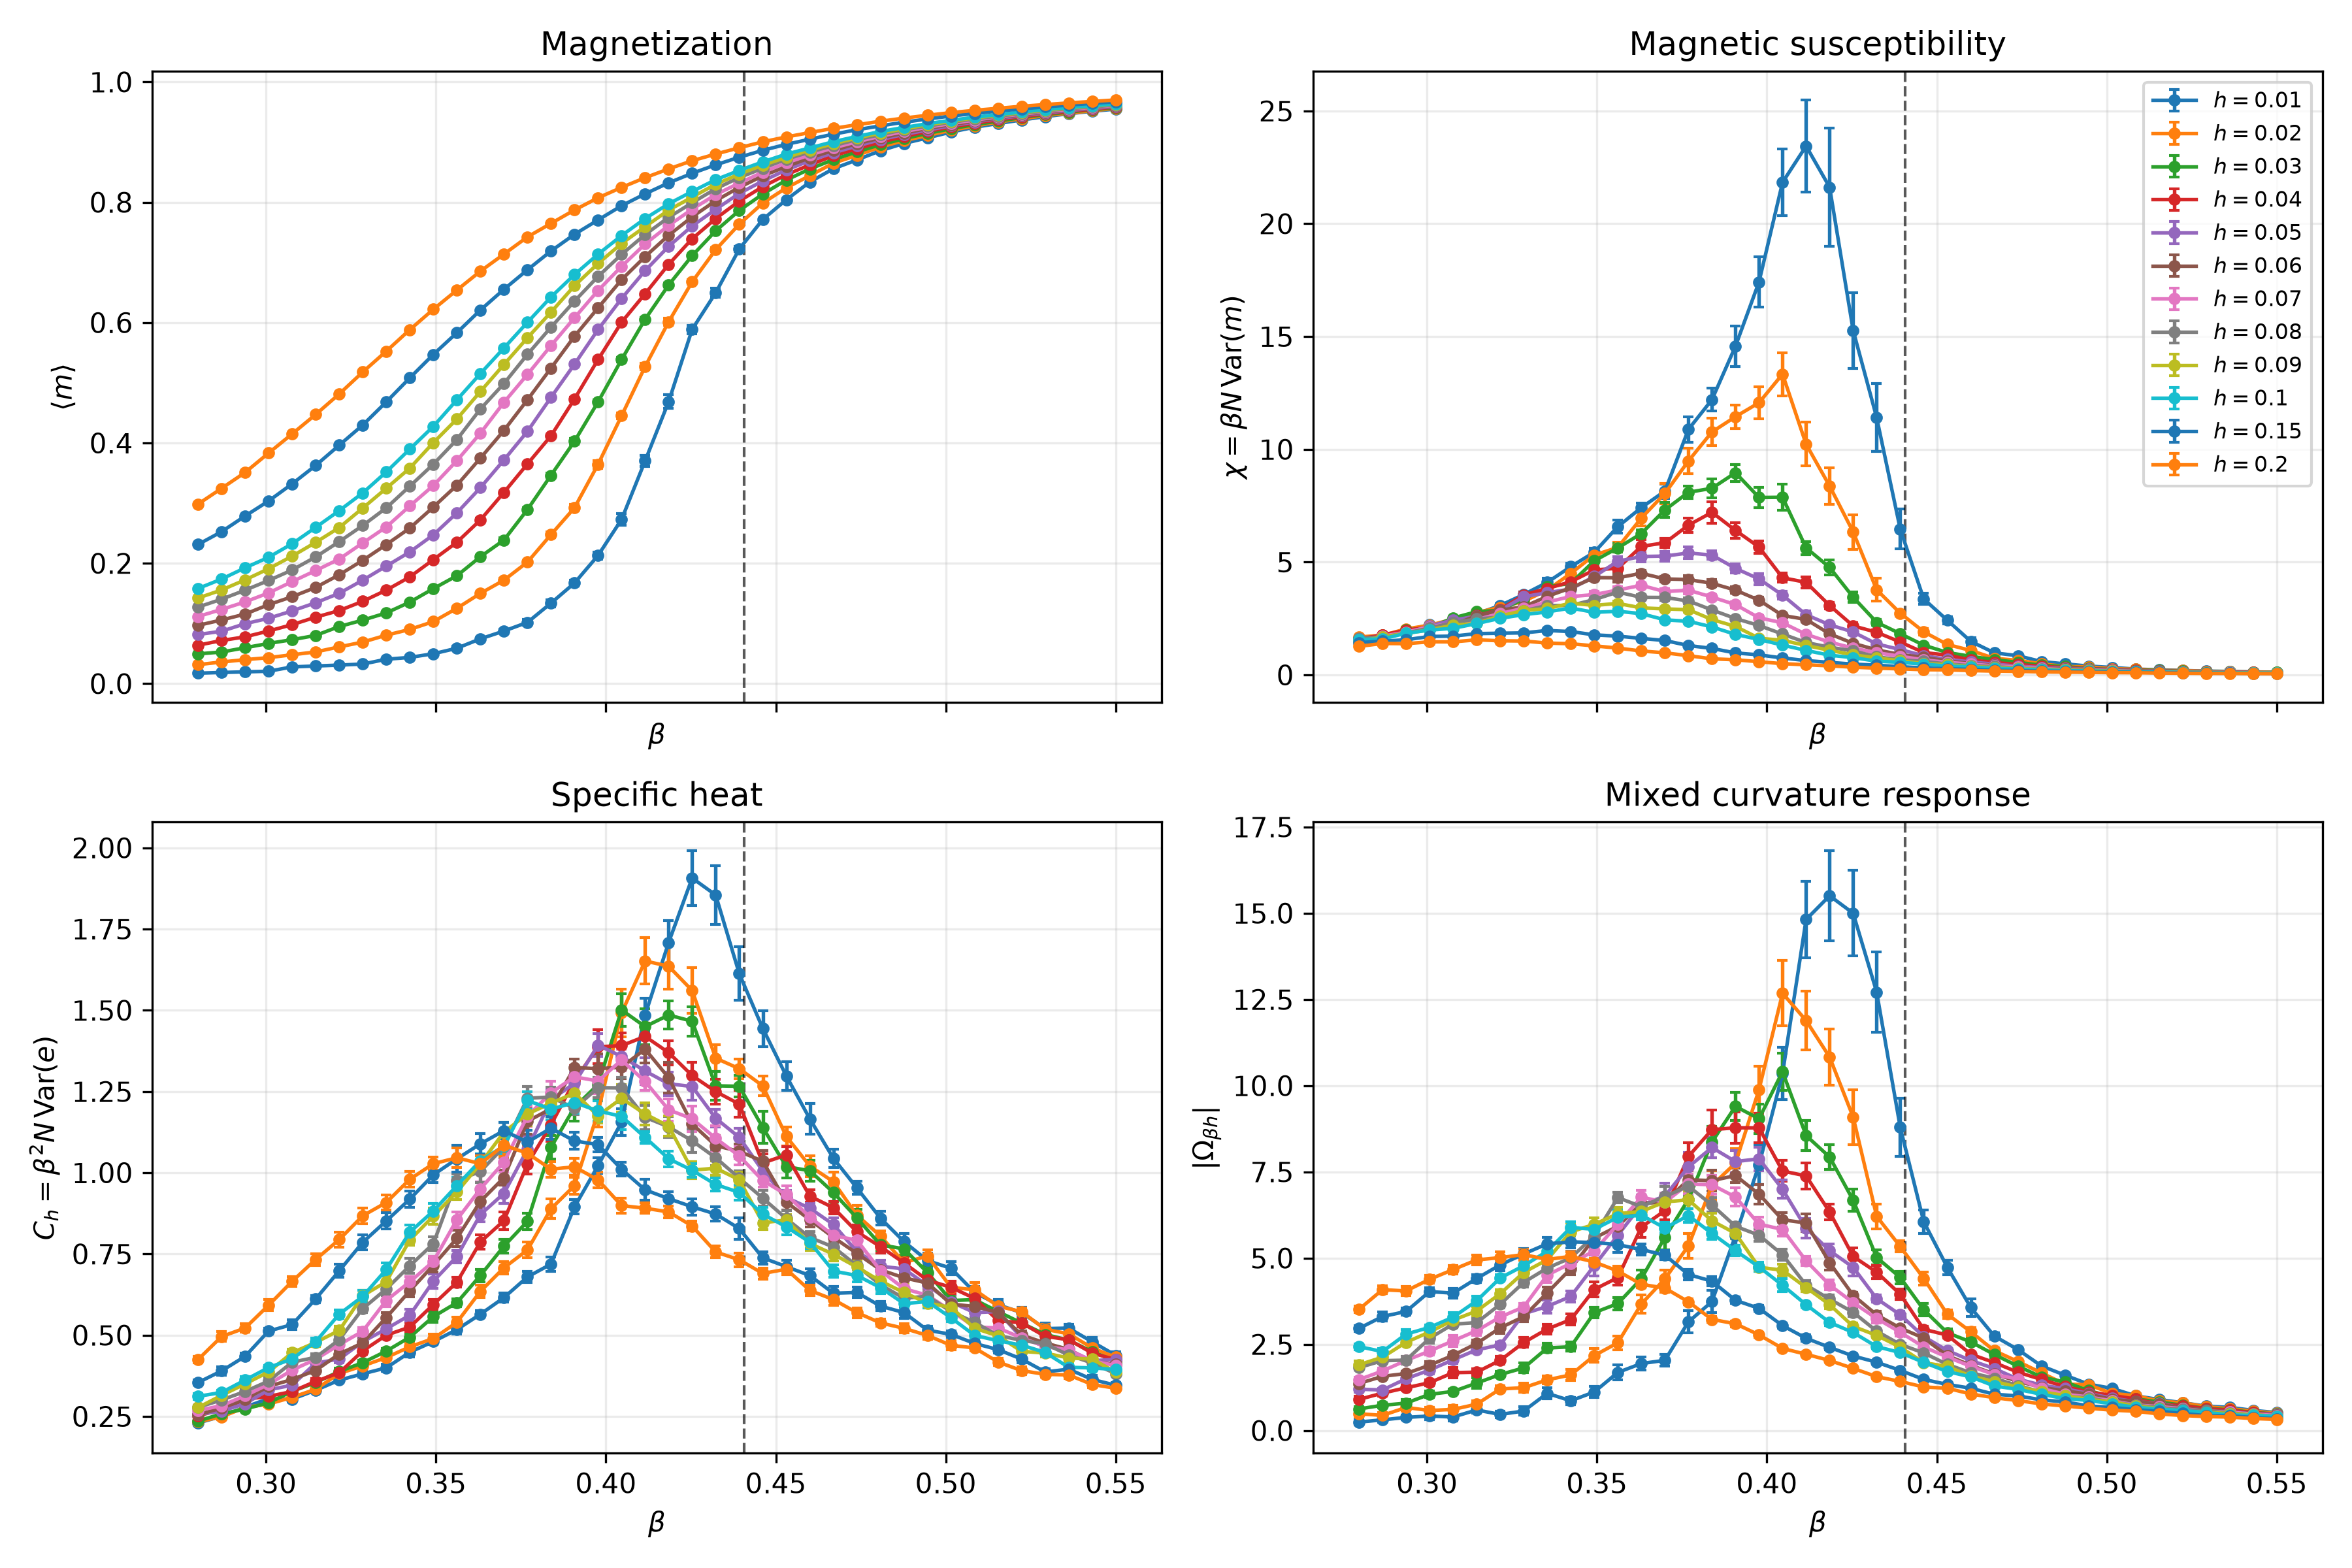
\includegraphics[width=\textwidth]{Figures/ising_cross_sections_all.png}
\caption{
Thermodynamic response functions of the two-dimensional Ising
model as functions of inverse temperature for several values
of the external magnetic field.
(a) Magnetization (m),
(b) magnetic susceptibility (\chi_T),
(c) heat capacity (C_h),
and
(d) mixed response
\(\Omega_{Th}=-\langle \delta E\delta M\rangle/(k_B T^2)\).
The first three panels represent the conventional response
functions associated with the diagonal elements of the
thermodynamic covariance matrix. The mixed response shown in
panel (d) arises from the off-diagonal covariance between
energy and magnetization fluctuations and therefore measures
the coupling between thermal and magnetic response sectors.
While all response functions exhibit enhanced behavior near the
critical region, the mixed response provides additional
information regarding the organization of correlated
fluctuations and serves as the fundamental quantity underlying
the response-geometric framework developed in this review.
}
\label{fig:ising_response_functions}
\end{figure*}
%=========================================================


Figure~\ref{fig:ising_response_functions} summarizes the
resulting response functions. Panels (a)–(c) show the
magnetization, susceptibility, and heat capacity for several
values of the external field. These quantities exhibit the
expected signatures of criticality, including enhanced response
near the Onsager critical point. Panel (d) shows the mixed
response \(\Omega_{Th}\). Although the mixed response displays
a pronounced peak near the critical region, its behavior is
qualitatively distinct from either the heat capacity or
susceptibility because it reflects the correlation between
energetic and magnetic fluctuations rather than fluctuations
within a single response sector.

At this stage it is useful to emphasize an important conceptual
shift. Conventional phase diagrams classify equilibrium states.
The quantities plotted in Fig.~\ref{fig:ising_response_functions}
instead characterize how those states respond to perturbations.
The resulting objects therefore belong naturally to a response
manifold rather than a state manifold. From this perspective,
the relevant question is no longer simply where a phase
transition occurs, but how response is distributed throughout
the surrounding thermodynamic landscape.



%=========================================================
\begin{figure*}[t]
\centering
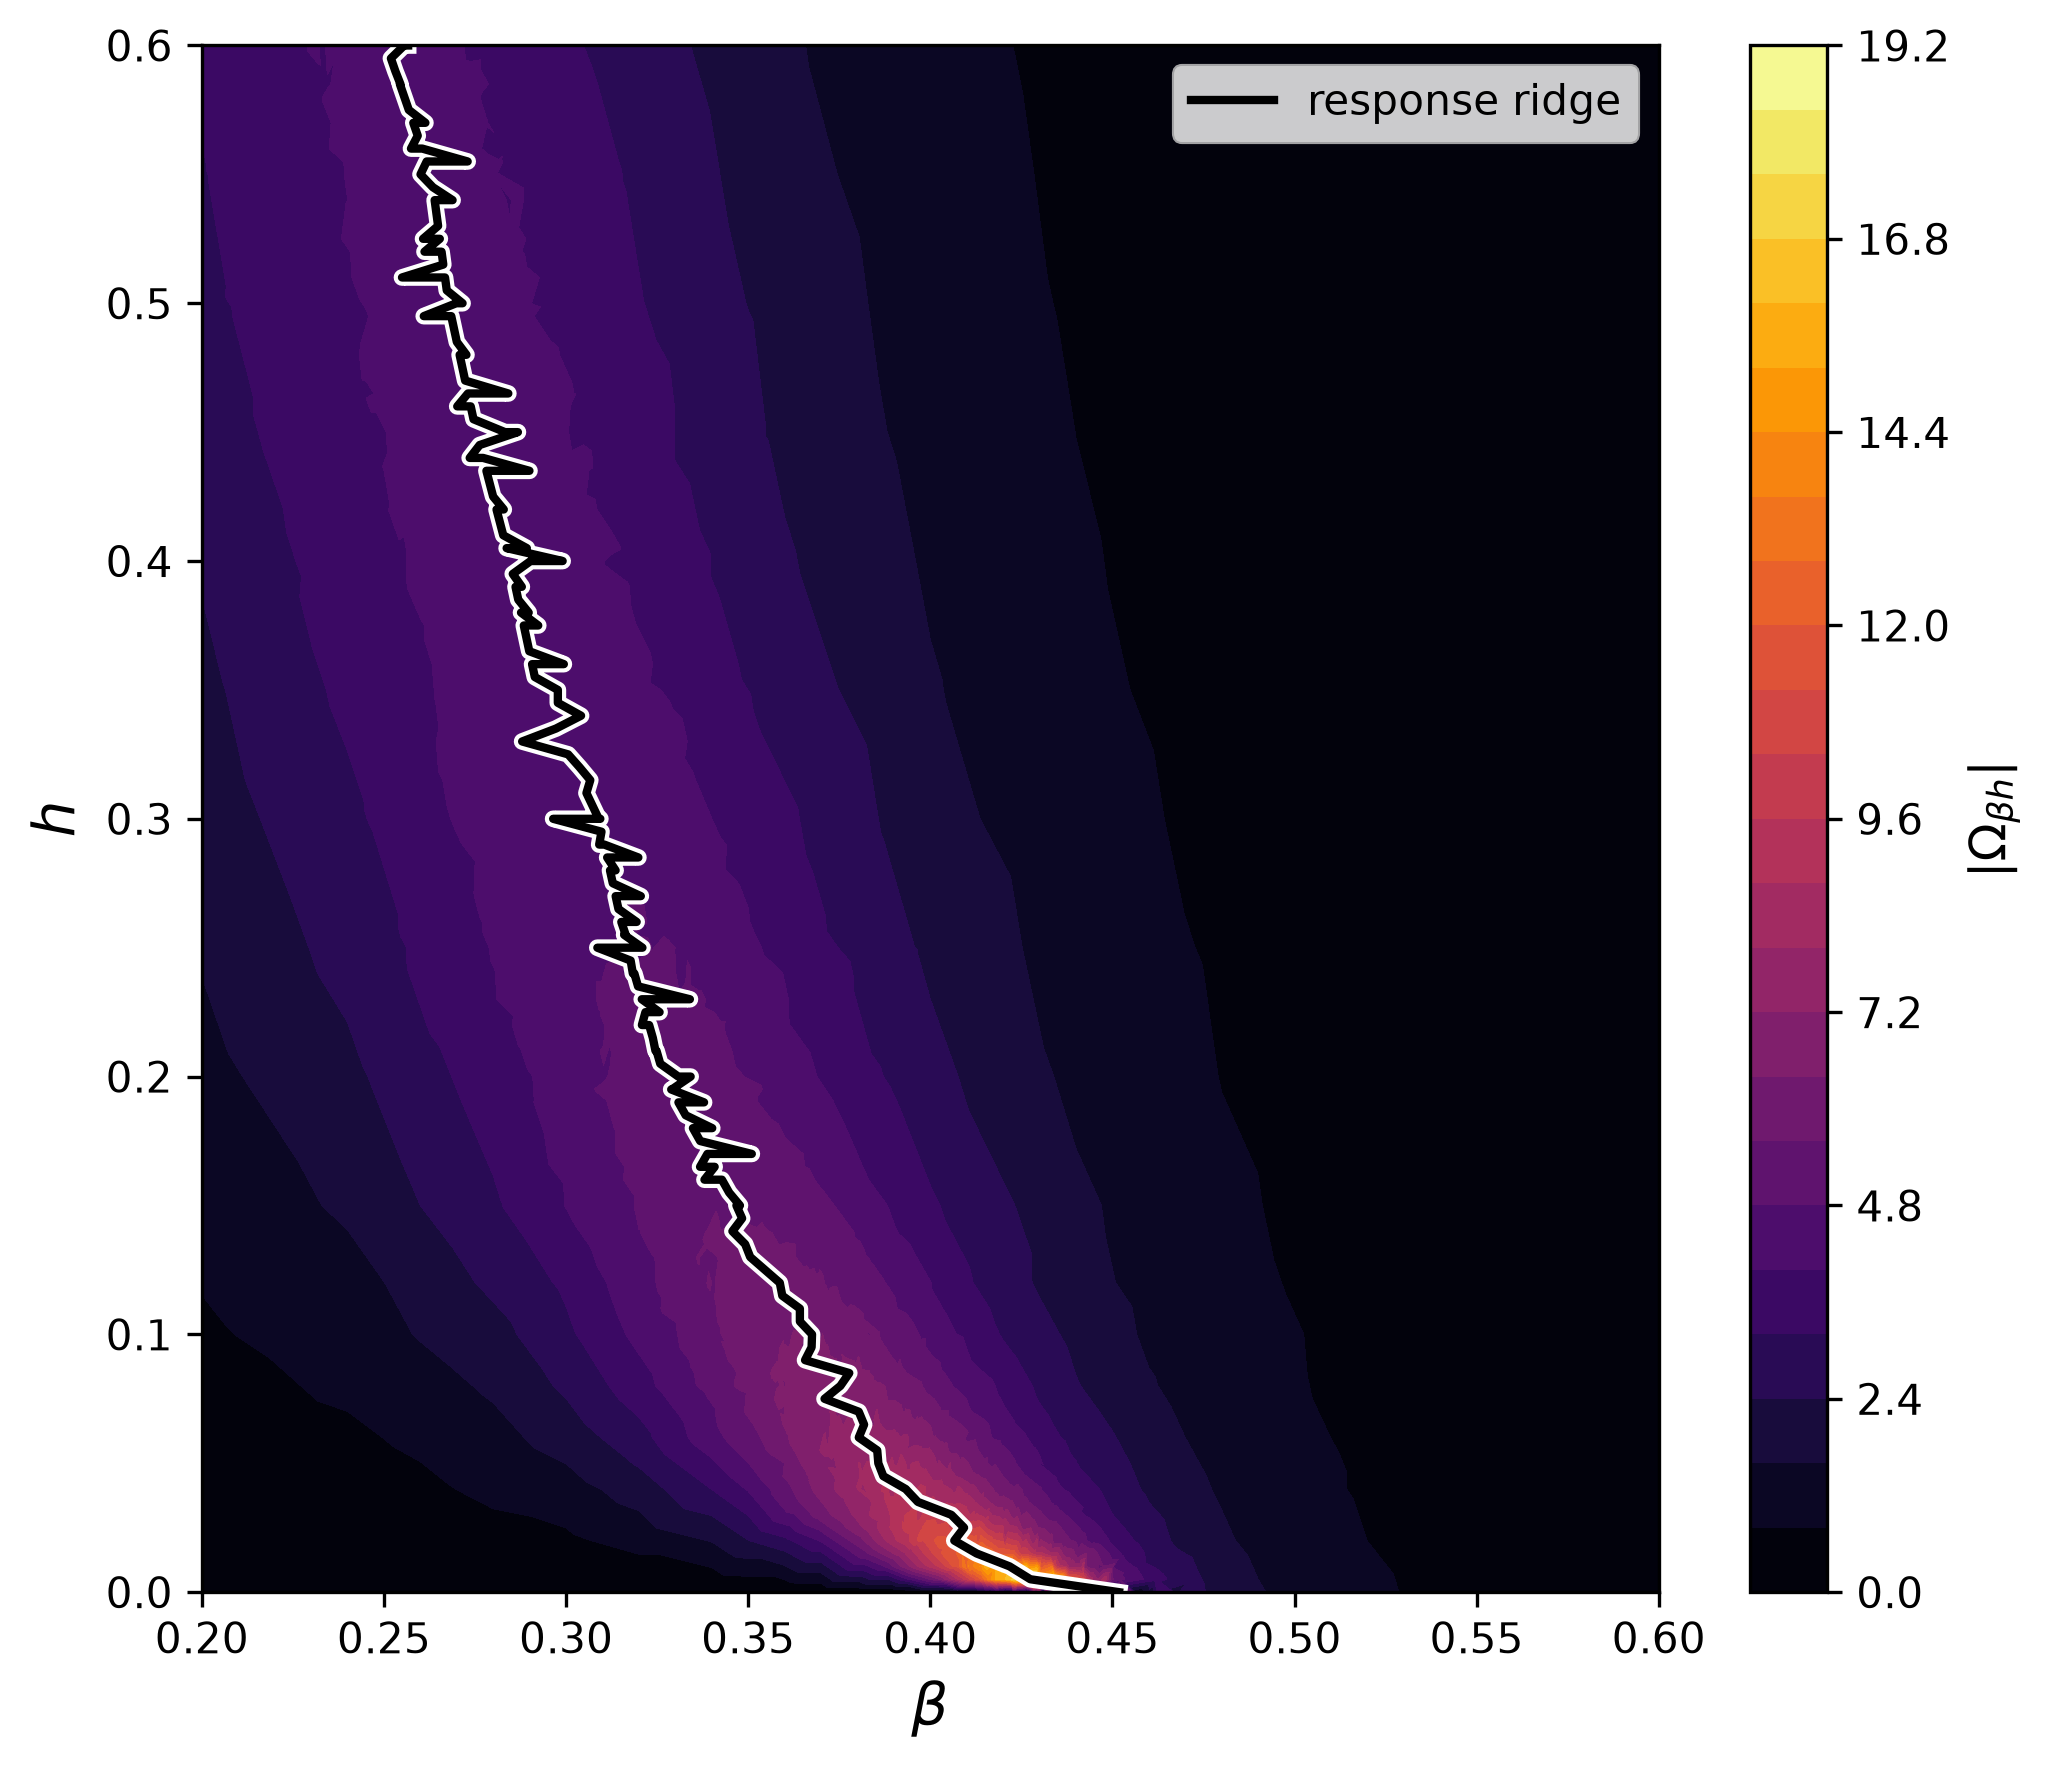
\includegraphics[width=0.85\textwidth]{Figures/ising_curvature_field_Omega.png}
\caption{
Mixed-response landscape
\(\Omega_{Th}(T,h)\)
for the two-dimensional Ising model together with the
extracted loci of maximal response.
The color scale indicates the magnitude of the mixed
fluctuation field, while the superimposed curves denote ridge
trajectories obtained from maxima of the response functions.
Unlike conventional phase diagrams, which classify equilibrium
states, the present construction characterizes how those
states respond to perturbations. The mixed-response ridge
extends well beyond the Onsager critical point into the
supercritical regime, revealing an extended pathway along
which thermal and magnetic fluctuations remain maximally
coupled. The existence of multiple ridge trajectories
associated with different response sectors demonstrates that
the supercritical region is organized by a hierarchy of
response structures rather than a single universal crossover
curve.
}
\label{fig:ising_ridge}
\end{figure*}
%=========================================================


This viewpoint becomes particularly illuminating when the mixed
response is evaluated throughout the full \((T,h)\) control
manifold. Figure~\ref{fig:ising_ridge} shows the resulting
response landscape \(\Omega_{Th}(T,h)\) together with the
extracted loci of maximal response. Rather than remaining
localized near the critical point, the mixed response organizes
into an extended ridge that persists deep into the
supercritical regime. The ridge identifies a pathway through
parameter space along which thermal and magnetic fluctuations
remain maximally coupled.

The appearance of such a structure is significant for several
reasons. First, it demonstrates that mixed fluctuations remain
organized far beyond the immediate vicinity of a thermodynamic
singularity. Second, the ridge provides a natural continuation
of collective response into the supercritical regime, where no
sharp phase boundary exists. Third, because the ridge is
constructed directly from experimentally accessible
fluctuations, it may be identified without reference to a
specific order parameter or symmetry-breaking mechanism.
Finally, the ridge reveals that phase diagrams may be viewed as
response landscapes whose geometry is encoded in the covariance
structure of the system.

An equally important result concerns the scaling behavior of the
response landscape. Analysis of the numerical data reveals that
the maxima of the heat capacity, magnetic susceptibility, and
mixed response obey distinct scaling laws as the critical
region is approached. The corresponding exponents differ,
indicating that the response matrix does not scale uniformly.
Instead, thermal, magnetic, and mixed fluctuation sectors are
amplified at different rates.

This observation admits a particularly natural geometric
interpretation. The covariance matrix defines a local
fluctuation ellipsoid whose principal axes describe the
dominant directions of thermodynamic response. If all response
sectors scaled identically, the covariance ellipsoid would
simply expand as criticality is approached. The numerical
results demonstrate that this is not the case. Because the
various response sectors exhibit distinct scaling behavior, the
covariance ellipsoid changes shape as well as size. The
response geometry therefore undergoes a continuous deformation,
with different response directions becoming dominant in
different regions of parameter space.

The loci of maximal response exhibit a similar hierarchy. The
susceptibility, heat-capacity, and mixed-response ridges follow
distinct trajectories through the control manifold, indicating
that the continuation of critical behavior into the
supercritical regime cannot be represented by a single
universal curve. Rather, the thermodynamic landscape contains a
family of response ridges associated with different fluctuation
sectors. From this perspective, the supercritical region is not
organized by a unique Widom line but by a hierarchy of response
trajectories reflecting different projections of the underlying
covariance structure.

The existence of multiple scaling sectors raises a natural
question. If the various response functions exhibit distinct
scaling behavior and define distinct ridge structures, should
they be regarded as independent coordinates of thermodynamic
response? Surprisingly, the numerical results suggest
otherwise.


%=========================================================
\begin{figure}[t]
\centering
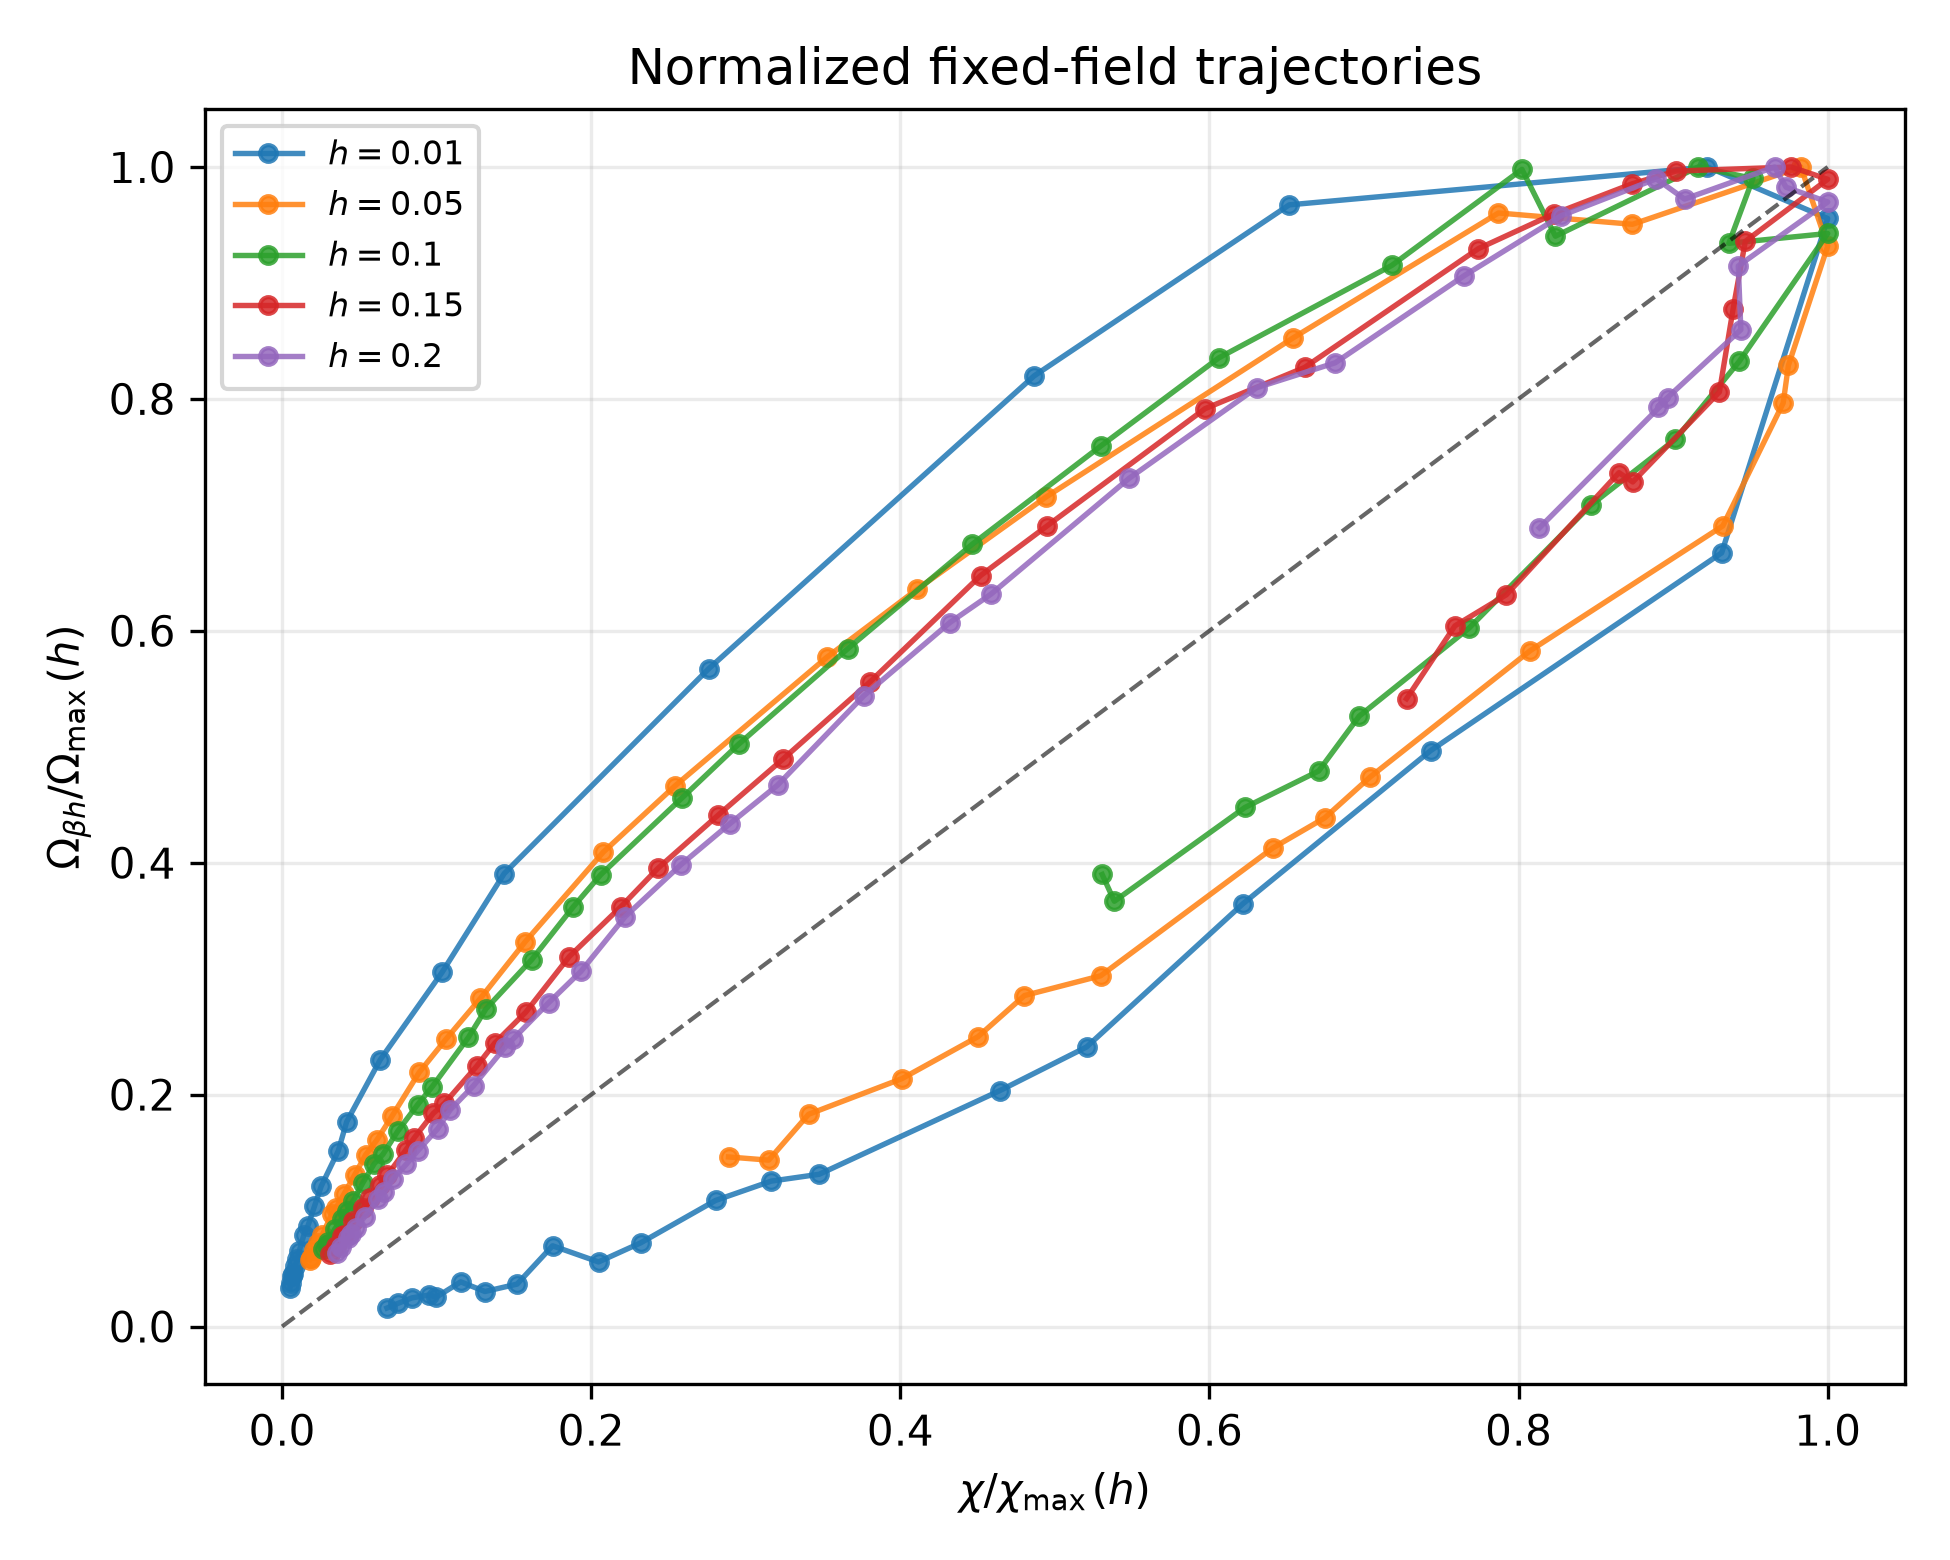
\includegraphics[width=\columnwidth]{Figures/omega_vs_chi_normalized_trajectories.png}
\caption{
Emergent response manifold in the two-dimensional Ising model.
Trajectories obtained for different values of the external
field are represented in terms of the normalized response
coordinates
\(\tilde{\chi}=\chi_T/\chi_{T,\mathrm{max}}\)
and
\(\tilde{\Omega}=\Omega_{Th}/\Omega_{Th,\mathrm{max}}\).
Despite corresponding to distinct thermodynamic trajectories
in the control manifold, the normalized responses collapse
onto an approximately universal curve. The result indicates
that the susceptibility and mixed response are not independent
observables but are constrained by an emergent geometric
relationship. The collapse provides evidence that the image of
the two-dimensional control manifold is concentrated near a
lower-dimensional object in response space, suggesting the
existence of an underlying response manifold that organizes
thermodynamic behavior across a broad range of temperatures
and fields.
}
\label{fig:response_manifold}
\end{figure}
%=========================================================

Figure~\ref{fig:response_manifold} shows representative
trajectories obtained by normalizing the response functions by
their respective maxima and representing them in response
space. Despite corresponding to different values of the
external field, the trajectories collapse onto a common curve
to a remarkable degree. The collapse suggests the existence of
an approximate functional relationship between the normalized
response variables and therefore indicates the emergence of a
low-dimensional response manifold.

The significance of this result is easily overlooked. A generic
mapping
\begin{equation}
\Phi :(T,h)
\longrightarrow (\chi_T,\Omega_{Th})
\end{equation}
from a two-dimensional control manifold into a two-dimensional
response space need not produce any collapse at all. One would
generically expect the image of the control manifold to fill a
substantial region of response space. Instead, the numerical
trajectories are concentrated near a lower-dimensional object.
The response functions therefore behave not as independent
coordinates but as quantities constrained by an emergent
geometric relationship.

Taken together, the covariance matrix, response ridges,
scaling hierarchies, and manifold collapse reveal a coherent
picture of thermodynamic response. The covariance matrix
defines the local fluctuation structure, mixed response
identifies the coupling between distinct fluctuation sectors,
the scaling hierarchy reveals the anisotropic amplification of
response, and the manifold collapse exposes a deeper geometric
constraint linking apparently independent observables.
Geometry therefore emerges not from the equilibrium states
themselves but from the organization of response. The Ising
model thus provides a concrete demonstration of the central
theme of this review: geometric structure is encoded not only
in states, but in how those states respond to external
perturbations.



\subsection{Response Geometry from Thermodynamic Potentials: Spin–Peierls and Orbital Models}

The Ising model provides perhaps the simplest realization of
response geometry, demonstrating that thermodynamic metrics and
mixed response functions may be reconstructed directly from
equilibrium fluctuations. More generally, however, many quantum
materials are described by microscopic Hamiltonians from which an
effective thermodynamic potential may be constructed explicitly.
This raises an important question: are the geometric structures
identified through statistical fluctuations peculiar to the
Ising model, or do they represent more general features of
thermodynamic response?

An ideal setting in which to address this question is provided
by spin–Peierls and related orbital models. These systems
occupy a central position in condensed-matter physics because
they naturally couple spin, orbital, electronic, and lattice
degrees of freedom through a dimerization instability. Their
importance extends well beyond the original description of
quasi-one-dimensional magnetic materials. Closely related
Hamiltonians underlie the Su–Schrieffer–Heeger (SSH) model of
conducting polymers, one-dimensional topological insulators,
correlated transition-metal oxides, synthetic quantum lattices,
photonic crystals, superconducting circuits, and other
engineered quantum materials. Although these systems are often
discussed from the perspective of topological band theory and
Berry phases, they also provide a rich arena for exploring the
geometry of thermodynamic response.

The conceptual distinction is an important one. Berry geometry
describes the evolution of quantum eigenstates under adiabatic
parameter variation, whereas the framework developed here is
concerned with the geometry of thermodynamic observables. The
relevant mathematical object is therefore not the wavefunction
or Bloch eigenstate, but the thermodynamic potential from which
the observable response is derived. This shift in perspective
allows the same microscopic Hamiltonian to be viewed through the
lens of equilibrium fluctuations, response functions, and
thermodynamic geometry.

Unlike the Ising model, where the response matrix was
reconstructed numerically from Monte Carlo covariances, the
models considered here admit an explicit microscopic
Hamiltonian. The thermodynamic response is obtained by
constructing the partition function and the corresponding
free-energy functional, from which all response quantities
follow by differentiation. As we shall show, this entirely
different computational route leads to remarkably similar
response landscapes, suggesting that the geometric structures
identified in the previous section are intrinsic properties of
thermodynamic response rather than artifacts of a particular
numerical methodology.

As a representative example, we consider the spin–Peierls
compound \ce{CuGeO3}, whose coupled spin, orbital, and lattice
degrees of freedom provide a realistic platform for illustrating
how response geometry emerges directly from a microscopic
Hamiltonian. In addition to its relevance for equilibrium
thermodynamics, the same Hamiltonian forms the starting point
for the nonequilibrium and spectroscopic developments discussed
in later sections, providing a direct bridge between
thermodynamic response, open quantum systems, and nonlinear
optical spectroscopy.


\subsubsection{Microscopic Spin–Orbital Hamiltonian}

To illustrate the construction of response geometry from a
microscopic theory, we consider a generic spin–orbital lattice
model representative of spin–Peierls materials such as
\ce{CuGeO3}. Rather than beginning from a phenomenological
Landau free-energy functional, we adopt a Hamiltonian that
explicitly incorporates the coupled spin, orbital, and lattice
degrees of freedom responsible for the thermodynamic response.
This formulation is sufficiently general to encompass not only
spin–Peierls compounds, but also the broader class of
Su–Schrieffer–Heeger (SSH) and dimerized lattice models that
appear throughout condensed-matter physics.

The microscopic Hamiltonian is written as
\begin{align}
H=H_{\mathrm{spin}}+H_{\mathrm{orb}}+H_{\mathrm{SO}}+H_{\mathrm{ph}}
+
H_{\mathrm{sp-ph}},
\end{align}
where the individual contributions describe magnetic exchange,
orbital energetics, spin–orbit coupling, lattice vibrations,
and spin–phonon interactions, respectively.

The magnetic degrees of freedom are described by an
antiferromagnetic Heisenberg chain,
\begin{align}
H_{\mathrm{spin}}
=
\sum_i
J_i(B,T),
\mathbf{S}i\cdot\mathbf{S}{i+1}
+
g\mu_BB
\sum_i
S_i^z,
\end{align}
where the nearest-neighbor exchange interaction is modulated by
the spin–Peierls distortion,
\begin{align}
J_i(B,T) =
J_0 + (-1)^i\delta(B,T).    
\end{align}

Unlike a conventional lattice parameter, the dimerization
amplitude \(\delta(B,T)\) is not fixed. Instead, it is an
emergent thermodynamic field determined self-consistently by
minimizing the equilibrium free-energy functional. As the
temperature and magnetic field vary, the equilibrium lattice
distortion evolves continuously over the thermodynamic control
manifold, modifying the exchange interaction and, consequently,
the magnetic excitation spectrum. The microscopic Hamiltonian
therefore depends implicitly upon the external control
variables through the equilibrium order parameter
\(\delta(B,T)\).

The orbital Hamiltonian describes the crystal-field splitting of
the \ce{Cu^{2+}} \ce{3d^9} manifold within the elongated
$D_{4h}$ ligand environment,
\begin{align}
H_{\mathrm{orb}}
=
\sum_{i,\alpha}
\epsilon_\alpha
n_{i\alpha},
\end{align}
while the spin–orbit interaction,
\begin{align}
H_{\mathrm{SO}}
=
\lambda
\sum_i
\mathbf{L}_i\cdot\mathbf{S}_i,
\end{align}
couples the spin and orbital sectors. Together with the lattice
Hamiltonian and the spin–phonon interaction, these terms
produce a microscopic description in which spin, orbital, and
structural degrees of freedom evolve cooperatively under the
influence of temperature and magnetic field.

Although the real-space representation most clearly exposes the
physical origin of the competing interactions, it is often
convenient to transform to reciprocal space. Introducing the
Fourier-transformed operators,
\begin{align}
c_{i\alpha}
=
\frac{1}{\sqrt{N}}
\sum_k
e^{ikR_i}
c_{k\alpha},
\end{align}
the Hamiltonian becomes
\begin{align}
H
=
\sum_k
\Psi_k^\dagger
\mathcal{H}(k;\delta(B,T))
\Psi_k,
\end{align}
where the Bloch Hamiltonian contains the dimerized exchange,
crystal-field splitting, and spin–orbit coupling in a form
closely analogous to the SSH model. In this representation, the
spin–Peierls distortion opens a gap at the Brillouin-zone
boundary while simultaneously modifying the spin and orbital
character of the low-energy quasiparticles.

This momentum-space representation provides the natural
starting point for constructing the partition function and the
equilibrium free-energy functional. More importantly, it
illustrates that the Hamiltonian is not merely parameterized by
the external thermodynamic variables but is itself reshaped by
the equilibrium order parameter \(\delta(B,T)\). The response
geometry developed below therefore reflects both the explicit
dependence of the free energy on the thermodynamic control
variables and the implicit evolution of the microscopic
Hamiltonian through the self-consistent lattice distortion.

\subsubsection{From the Spin--Orbital Hamiltonian to a Free-Energy Functional}
The self-consistent nature of the spin--Peierls distortion makes
the construction of the thermodynamic potential especially
important. The Hamiltonian depends on the external control
variables both explicitly, through the Zeeman coupling to the
magnetic field, and implicitly through the equilibrium
dimerization amplitude \(\delta(T,h)\). The response geometry
therefore cannot be obtained by differentiating microscopic
Hamiltonian parameters alone. Instead, it emerges only after the
equilibrium thermodynamic potential has been constructed.
For a fixed value of the dimerization amplitude, the
momentum-space Hamiltonian defines the partition function
\begin{align}
Z(T,h;\delta)
=
\mathrm{Tr}
\exp\!\left[
-\beta H(h;\delta)
\right].
\end{align}
In the band representation this may be written as
\begin{align}
Z(T,h;\delta)
=
\prod_{k,n}
\left[
1+
\exp\!\left(
-\beta\varepsilon_n(k;h,\delta)
\right)
\right],
\end{align}
where \(\varepsilon_n(k;h,\delta)\) denotes the eigenvalues of
the Bloch Hamiltonian
\(\mathcal{H}(k;h,\delta)\).
The corresponding electronic contribution to the free energy is
\begin{align}
F_{\rm el}(T,h;\delta)
=
-k_BT
\sum_{k,n}
\ln\!\left[
1+
\exp\!\left(
-\beta\varepsilon_n(k;h,\delta)
\right)
\right].
\end{align}
The total free energy contains both the electronic and elastic
contributions,
\begin{align}
F(T,h;\delta)
=
F_{\rm el}(T,h;\delta)
+
\frac{K}{2}\delta^2
+
F_{\rm ph}(T),
\end{align}
where \(K\) is the effective stiffness of the Peierls mode and
\(F_{\rm ph}\) denotes the remaining phonon contribution.
The equilibrium dimerization is determined by minimizing the
free energy at each point of the thermodynamic control manifold,
\begin{align}
\left.
\frac{\partial F(T,h;\delta)}
{\partial\delta}
\right|_{\delta=\delta_\ast(T,h)}
=
0,
\end{align}
so that
\begin{align}
\delta(T,h)
=
\delta_\ast(T,h).
\end{align}
The free-energy minimization therefore defines the mapping
\[
(T,h)
\longrightarrow
\delta_\ast(T,h),
\]
so that the equilibrium order parameter becomes an emergent
field over the thermodynamic control manifold.
The physical thermodynamic potential is consequently
\begin{align}
F_{\rm eq}(T,h)
=
F\!\left(T,h;\delta_\ast(T,h)\right).
\end{align}
This distinction is essential. The response functions are not
obtained by holding the microscopic dimerization fixed, but by
differentiating the equilibrium free energy after the order
parameter has been determined self-consistently. Consequently,
the thermodynamic derivatives contain both explicit derivatives
with respect to the external control variables and implicit
contributions arising from the evolution of
\(\delta_\ast(T,h)\).
Because \(F_{\rm eq}(T,h)\) is a thermodynamic state function,
its differential is exact,
\begin{align}
dF_{\rm eq}
=
-S\,dT
-
m\,dh.
\end{align}
The entropy and magnetization follow immediately from
\begin{align}
S
&=
-
\left(
\frac{\partial F_{\rm eq}}
{\partial T}
\right)_h,
\\
m
&=
-
\left(
\frac{\partial F_{\rm eq}}
{\partial h}
\right)_T.
\end{align}
The second derivatives define the thermodynamic response
functions,
\begin{align}
C_h
&= - T
\left(
\frac{\partial^2F_{\rm eq}}
{\partial T^2}
\right)_h,
\\
\chi_T
&=
-\left(
\frac{\partial^2F_{\rm eq}}
{\partial h^2}
\right)_T,
\\
\Omega_{Th}
&=
-
\frac{\partial^2F_{\rm eq}}
{\partial T\,\partial h}
=
-
\left(
\frac{\partial m}{\partial T}
\right)_h
=
-
\left(
\frac{\partial S}{\partial h}
\right)_T.
\end{align}
Since the numerical calculations are performed in terms of the
inverse temperature,
\(\beta=(k_BT)^{-1}\),
the response maps presented below are expressed as
\begin{align}
\Omega_{\beta h}
=
\left(
\frac{\partial m}
{\partial\beta}
\right)_h,
\end{align}
which differs from \(\Omega_{Th}\) only through the Jacobian
relating derivatives with respect to \(T\) and \(\beta\).
This is the quantity shown in
Fig.~\ref{fig:cugeo3_response}.

The construction developed here illustrates an important
principle that extends well beyond the specific spin--Peierls
model. The response geometry is not inherited directly from the
microscopic Hamiltonian, but from the thermodynamic potential
constructed from that Hamiltonian. The role of the microscopic
model is to define the statistical ensemble and, through the
partition function, the equilibrium free-energy functional.
Once the equilibrium order parameter has been determined
self-consistently, the exact differential of the resulting
thermodynamic potential generates the complete response
structure through its first and second derivatives.
In the present model, the spin--Peierls order parameter
\(\delta_\ast(T,h)\) serves as an emergent thermodynamic field
defined over the control manifold. The microscopic Hamiltonian
therefore depends implicitly upon the thermodynamic state,
reflecting the self-consistent evolution of the equilibrium
lattice distortion. Consequently, the response functions encode
not only the explicit dependence of the free energy on the
external control variables, but also the collective
reorganization of the underlying spin, orbital, and lattice
degrees of freedom.

This distinction is central to the geometric framework developed
throughout this review. Different physical systems may employ
very different microscopic Hamiltonians and computational
methods---Monte Carlo sampling in the Ising model,
self-consistent free-energy minimization in the spin--Peierls
model, or nonequilibrium steady-state density matrices in open
quantum systems. Nevertheless, the geometric objects themselves
always derive from the thermodynamic or dynamical response
rather than from the microscopic representation used to compute
it. Response geometry is therefore a property of the response
manifold, not of the Hamiltonian from which that response is
obtained.
\begin{figure*}[t]
\centering
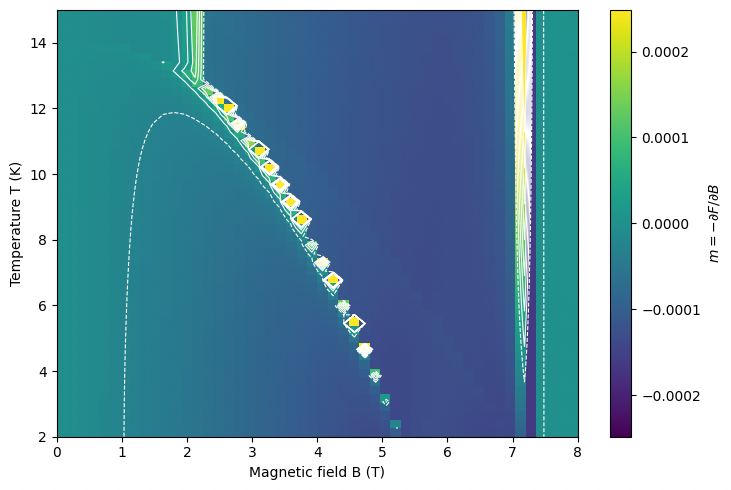
\includegraphics[width=0.48\textwidth]{Figures/CuGeO3-mag.png}
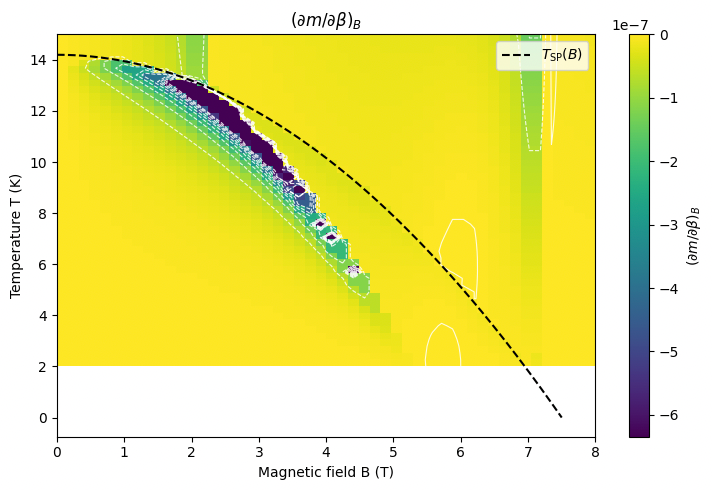
\includegraphics[width=0.48\textwidth]{Figures/CuGeO3-mixed-deriv.png}
\caption{
Response geometry of the spin--Peierls model for \ce{CuGeO3}.
(a) Magnetization landscape \(\langle m\rangle(B,T)\) over the
magnetic-field--temperature control manifold.
(b) Mixed thermal-field response
\((\partial m/\partial \beta)_B\), obtained by differentiating
the free-energy functional. The dashed curve denotes the
spin--Peierls transition scale \(T_{\rm SP}(B)\). The mixed
response develops an extended ridge that tracks the reorganization
of the spin--Peierls state under magnetic field. Unlike the Ising
case, where the response geometry is reconstructed from Monte Carlo
covariances, here the same geometric structure is obtained directly
from a thermodynamic potential.
}
\label{fig:cugeo3_response}
\end{figure*}

\subsection{Rewrite: Phenomenological Spin--Peierls Model for \ce{CuGeO3}}
As a second example of equilibrium response geometry, we consider
a phenomenological spin--Peierls model motivated by \ce{CuGeO3}.
Unlike the Ising model, where the response functions were obtained
from Monte Carlo sampling of equilibrium fluctuations, the present
calculation proceeds by constructing a microscopic free-energy model
and differentiating the resulting thermodynamic potential. This
provides a complementary route to response geometry: the response
manifold is generated not from sampled covariances, but from a
field- and temperature-dependent free-energy landscape.

The model combines an SSH-like orbital band Hamiltonian with a
phenomenological spin--Peierls order parameter. The total free energy
is written as
\begin{align}
F(T,B)
=
F_{\rm band}(T,B)
+
F_{\rm spin}(T,B)
+
F_{\rm SP}(T,B).
\end{align}
The band contribution is obtained from a two-sublattice Bloch
Hamiltonian with five real \(d\)-orbitals,
\[
(d_{xy},d_{yz},d_{xz},d_{x^2-y^2},d_{z^2}),
\]
including ligand-field splittings, spin--orbit coupling, Zeeman
coupling, and an SSH-like hopping alternation. The local Hamiltonian
has the form
\begin{align}
H_{\rm loc}
=
H_{\rm lf}
+
\lambda_{\rm SO}\,\mathbf L\cdot\mathbf S
+
\mu_B
\left(
k_{\rm orb}\mathbf L
+
g_s\mathbf S
\right)\cdot\mathbf B,
\end{align}
where the orbital angular momentum matrices are represented in the
real \(d\)-orbital basis.
The Bloch Hamiltonian is defined on a two-sublattice unit cell as
\begin{align}
\mathcal H(k)
=
\begin{pmatrix}
H_{\rm loc} & Q(k)\\
Q^\dagger(k) & H_{\rm loc}
\end{pmatrix},
\end{align}
with
\begin{align}
Q(k)
=
T_1+T_2 e^{-ik},
\qquad
T_1=(1+\delta)T_0,
\qquad
T_2=(1-\delta)T_0.
\end{align}
Here \(T_0\) contains orbital-diagonal hopping amplitudes and selected
inter-orbital hopping terms. The hopping dimerization is tied to the
spin--Peierls order parameter through
\begin{align}
\delta_t(T,B)
=
\delta_{t0}\,\phi(T,B).
\end{align}
For eigenvalues \(\varepsilon_n(k)\) of \(\mathcal H(k)\), the band
free energy is evaluated as
\begin{align}
F_{\rm band}
=
-\frac{1}{\beta}
\frac{1}{N_k}
\sum_{k,n}
\ln
\left[
1+
\exp\left(-\beta \varepsilon_n(k)\right)
\right].
\end{align}
The spin--Peierls order parameter is introduced phenomenologically
using a mean-field field-dependent transition temperature,
\begin{align}
T_{\rm SP}(B)
=
T_{\rm SP}^{0}
\left[
1-\left(\frac{B}{B_c}\right)^2
\right],
\end{align}
and
\begin{align}
\phi(T,B)
=
\sqrt{1-\frac{T}{T_{\rm SP}(B)}}
\sqrt{1-\left(\frac{B}{B_c}\right)^2},
\end{align}
for \(T<T_{\rm SP}(B)\) and \(|B|<B_c\), with
\(\phi(T,B)=0\) otherwise. The corresponding spin--Peierls gap is
\begin{align}
\Delta_{\rm SP}(T,B)
=
\Delta_{\rm SP}^{0}\phi(T,B).
\end{align}
The spin excitation spectrum is modeled by
\begin{align}
E_0(k)
=
\sqrt{
\Delta_{\rm SP}^2
+
\epsilon_k^2
},
\qquad
\epsilon_k
=
J_1\cos k+J_2\cos(2k),
\end{align}
with Zeeman-shifted branches
\begin{align}
E_{\pm}(k)
=
E_0(k)
\pm
g_s\mu_B B.
\end{align}
The spin contribution to the free energy is then
\begin{align}
F_{\rm spin}
=
\frac{1}{\beta}
\frac{1}{N_k}
\sum_k
\left[
\ln\left(1-e^{-\beta E_+(k)}\right)
+
\ln\left(1-e^{-\beta E_-(k)}\right)
\right].
\end{align}
Finally, a Landau-like stabilization term is included,
\begin{align}
F_{\rm SP}
=
-K_{\rm SP}
\left(\Delta_{\rm SP}^{0}\right)^2
\phi^2(T,B),
\end{align}
which favors the ordered spin--Peierls state below the transition
line.

The thermodynamic response functions are obtained by numerical
differentiation of the resulting free energy. The magnetization proxy
is
\begin{align}
m(T,B)
=
-
\left(
\frac{\partial F}{\partial B}
\right)_T,
\end{align}
and the mixed thermal-field response is
\begin{align}
R_\beta(T,B)
=
\left(
\frac{\partial m}{\partial\beta}
\right)_B.
\end{align}
This is the response field plotted in
Fig.~\ref{fig:cugeo3_response}. We also compute the magnetic
susceptibility proxy
\begin{align}
\chi_B(T,B)
=
\left(
\frac{\partial m}{\partial B}
\right)_T.
\end{align}
A Widom-line-like crossover ridge is extracted by locating, at each
fixed magnetic field, the temperature where the magnitude of the
mixed response is maximal,
\begin{align}
T^\ast(B)
=
\operatorname*{arg\,max}_{T}
\left|
R_\beta(T,B)
\right|.
\end{align}
The present calculation should be interpreted as a phenomenological
spin--Peierls response model rather than a fully self-consistent
minimization over the lattice distortion. The order parameter
\(\phi(T,B)\) is specified by the mean-field ansatz above and then
used to construct the band, spin, and Landau contributions to the
free energy. The response geometry is inherited from the resulting
thermodynamic potential \(F(T,B)\). Thus, as in the Ising model, the
geometric quantities are properties of the response manifold, not of
the microscopic Hamiltonian alone.


\subsection{Summary}
The examples considered in this section demonstrate that response geometry is independent of the computational framework used to obtain the thermodynamic potential. Whether reconstructed from equilibrium fluctuations or derived analytically from a microscopic free-energy functional, the same geometric structures emerge from the response manifold. This observation naturally raises the question of whether an analogous construction exists for systems that possess no equilibrium thermodynamic potential. The answer, developed in the following sections, is affirmative. In open quantum systems the free energy is replaced by the nonequilibrium steady-state density operator, and the exact differential of equilibrium thermodynamics gives way to a response one-form whose non-exactness generates an intrinsic curvature. The resulting framework may therefore be viewed as the quantum generalization of response geometry developed here.



\section{From Green--Kubo Response to Response Geometry}
\label{sec:kubo_response_geometry}
The preceding sections emphasized thermodynamic response as
the origin of metric and curvature structures in equilibrium and
near-critical systems. We now connect this viewpoint to the
standard language of response theory. The purpose is not to
replace Green--Kubo or nonlinear response theory, but to
reinterpret them geometrically. Green functions, susceptibilities,
response tensors, and nonlinear response functions remain the
central physical objects. Response geometry emerges when one
asks how these response objects themselves vary over a manifold
of external controls.

\subsection{Linear Response and Retarded Green Functions}
Consider a system perturbed by a weak external field \(f(t)\)
coupled to an operator \(B\),
\begin{align}
H(t)=H_0-f(t)B .
\end{align}
To first order in the perturbation, the induced change in the
expectation value of an observable \(A\) is
\begin{align}
\delta\langle A(t)\rangle
=
\int_{-\infty}^{\infty}dt'\,
\chi_{AB}(t-t')f(t'),
\end{align}
where causality requires \(\chi_{AB}(t-t')=0\) for
\(t<t'\). In quantum mechanics the response function is the
retarded Green function
\begin{align}
\chi_{AB}(t)
=
-\frac{i}{\hbar}\Theta(t)
\langle [A(t),B(0)]\rangle_0 .
\label{eq:kubo_response}
\end{align}
Equation~\eqref{eq:kubo_response} is the Kubo formula. It
expresses a measurable susceptibility in terms of an equilibrium
correlation function and therefore provides the microscopic
origin of linear response.
In frequency space,
\begin{align}
\delta\langle A(\omega)\rangle
=
\chi_{AB}(\omega)f(\omega),
\end{align}
so that the susceptibility is the linear map taking a perturbing
field into an observable response. From the perspective of this
review, this is the first geometric step: response is not simply a
number, but a bilinear object relating a direction in perturbation
space to a direction in observable space.

\subsection{From Green--Kubo Response to Geometric Response Theory}
\label{sec:GreenKuboGeometry}
Linear response theory provides the natural starting point for a
geometric description of thermodynamic and quantum response.
Traditionally, the Green--Kubo formalism relates transport
coefficients and susceptibilities to equilibrium correlation
functions, while the fluctuation--dissipation theorem connects
these response functions to spontaneous fluctuations in
equilibrium. The geometric framework developed in this review
extends this picture by showing that the response tensor naturally
decomposes into reciprocal and nonreciprocal sectors, giving rise
to a metric geometry associated with fluctuations and a curvature
geometry associated with cyclic transport.
Consider an open quantum system governed by the parameter-dependent
Liouvillian
%
\begin{equation}
\dot{\rho}
=
\mathcal L(\bm{\lambda})\rho,
\end{equation}
%
with stationary state satisfying
%
\begin{equation}
\mathcal L(\bm{\lambda})
\rho_{\rm ss}
=
0.
\end{equation}
%
For a family of control parameters
$\bm{\lambda}=\{\lambda^\mu\}$,
we define the generalized forces
%
\begin{equation}
O_\mu
=
\frac{\partial H}
{\partial\lambda^\mu},
\end{equation}
%
and the corresponding response one-form
%
\begin{equation}
A_\mu
=
\mathrm{Tr}
\left(
\rho_{\rm ss}
O_\mu
\right)
=
\langle O_\mu\rangle_{\rm ss}.
\end{equation}
%
The exterior derivative of this one-form defines the response
curvature,
%
\begin{equation}
F_{\mu\nu}
=
\partial_\mu A_\nu
-
\partial_\nu A_\mu,
\end{equation}
%
whose surface integral gives the geometric work accumulated over a
closed quasistatic control cycle,
%
\begin{equation}
W
=
\oint A
=
\iint_\Sigma
F.
\end{equation}
To connect this geometric construction with response theory,
differentiate the stationary-state condition,
%
\begin{equation}
\mathcal L
\rho_{\rm ss}
=
0,
\end{equation}
%
to obtain
%
\begin{equation}
\mathcal L
\,
\partial_\mu\rho_{\rm ss}
=
-
(\partial_\mu\mathcal L)
\rho_{\rm ss}.
\end{equation}
%
Introducing the Drazin inverse of the Liouvillian,
%
\begin{equation}
\mathcal L^+,
\end{equation}
%
gives
%
\begin{equation}
\partial_\mu\rho_{\rm ss}
=
-
\mathcal L^+
(\partial_\mu\mathcal L)
\rho_{\rm ss}.
\end{equation}
For Hamiltonian control parameters,
%
\begin{equation}
(\partial_\mu\mathcal L)\rho
=
-i
[O_\mu,\rho],
\end{equation}
%
and using the integral representation
%
\begin{equation}
\mathcal L^+
=
-
\int_0^\infty
dt\,
e^{\mathcal Lt},
\end{equation}
%
one finds
%
\begin{equation}
\partial_\mu\rho_{\rm ss}
=
-i
\int_0^\infty
dt\,
e^{\mathcal Lt}
[O_\mu,\rho_{\rm ss}],
\end{equation}
%
so that
%
\begin{equation}
\partial_\mu A_\nu
=
-i
\int_0^\infty
dt\,
\mathrm{Tr}
\left[
O_\nu
e^{\mathcal Lt}
[O_\mu,\rho_{\rm ss}]
\right].
\end{equation}
The quantum regression theorem identifies the Liouvillian
propagator appearing above with experimentally accessible
two-time correlation functions,
%
\begin{equation}
\mathrm{Tr}
\left[
O_\nu
e^{\mathcal Lt}
(O_\mu\rho_{\rm ss})
\right]
=
\langle
O_\nu(t)
O_\mu(0)
\rangle_{\rm ss},
\end{equation}
%
leading to
%
\begin{equation}
\partial_\mu A_\nu
=
-i
\int_0^\infty
dt\,
\langle
[O_\nu(t),O_\mu(0)]
\rangle_{\rm ss}.
\end{equation}
%
The response curvature therefore becomes
%
\begin{equation}
\boxed{
F_{\mu\nu}
=
-i
\int_0^\infty
dt
\left[
\langle
[O_\nu(t),O_\mu(0)]
\rangle
-
\langle
[O_\mu(t),O_\nu(0)]
\rangle
\right].
}
\label{eq:CurvatureCorrelation}
\end{equation}
Equation~(\ref{eq:CurvatureCorrelation}) establishes that the
geometric curvature is the integrated antisymmetric correlation
function of the generalized forces.
This connection becomes particularly transparent upon introducing
the retarded susceptibility,
%
\begin{equation}
\chi_{\mu\nu}^{R}(t)
=
-i
\theta(t)
\langle
[O_\mu(t),O_\nu(0)]
\rangle,
\end{equation}
%
whose zero-frequency limit is
%
\begin{equation}
\chi_{\mu\nu}^{R}(0)
=
-i
\int_0^\infty
dt\,
\langle
[O_\mu(t),O_\nu(0)]
\rangle.
\end{equation}
%
The response curvature may therefore be written as
%
\begin{equation}
\boxed{
F_{\mu\nu}
=
\chi_{\nu\mu}^{R}(0)
-
\chi_{\mu\nu}^{R}(0),
}
\label{eq:CurvatureKubo}
\end{equation}
%
showing that the curvature is precisely the antisymmetric
zero-frequency response tensor.
Equations~(\ref{eq:CurvatureCorrelation}) and
(\ref{eq:CurvatureKubo}) suggest a natural geometric
decomposition of response theory. The reciprocal sector of the
response tensor is generated by the symmetric correlation
functions,
%
\begin{equation}
G_{\mu\nu}
\sim
\int_0^\infty
dt\,
\left\langle
\{
\delta O_\mu(t),
\delta O_\nu(0)
\}
\right\rangle,
\end{equation}
%
while the nonreciprocal sector is generated by the corresponding
commutator correlations,
%
\begin{equation}
F_{\mu\nu}
\sim
\int_0^\infty
dt\,
\left\langle
[
\delta O_\mu(t),
\delta O_\nu(0)
]
\right\rangle.
\end{equation}
From this perspective, the Green--Kubo formalism naturally
decomposes into two complementary geometric sectors. The symmetric
sector determines a response metric that characterizes
distinguishability, fluctuations, and susceptibility, while the
antisymmetric sector determines a response curvature that
characterizes circulation, geometric work, and nonreciprocal
transport. Response geometry therefore extends the conventional
fluctuation--dissipation theorem by recognizing that reciprocal
and nonreciprocal response are complementary geometric
manifestations of the same underlying correlation functions.


\subsection{Reciprocity, Onsager Symmetry, and Geometric Response}
\label{sec:ReciprocityGeometry}
The preceding discussion shows that response functions admit a
natural geometric interpretation. This perspective becomes
particularly transparent when viewed through the lens of Onsager
reciprocity. In systems satisfying microscopic reversibility, the
static susceptibility is reciprocal,
%
\begin{equation}
\chi_{\mu\nu}
=
\chi_{\nu\mu},
\end{equation}
%
reflecting the underlying symmetry imposed by detailed balance.
The response tensor is therefore entirely symmetric and may be
identified with a Riemannian metric on the control manifold. The
resulting geometry is one of distinguishability, fluctuations,
and susceptibility, and corresponds to the familiar equilibrium
geometries introduced by Weinhold and Ruppeiner.

Away from equilibrium, however, microscopic reversibility need
not hold. External driving, coherent environmental coupling,
nonequilibrium steady states, or measurement backaction may all
break reciprocity, producing an antisymmetric sector of the
response tensor. Rather than viewing this contribution as a small
correction to the reciprocal response, it is more natural to
regard it as defining an independent geometric structure.

Accordingly, we decompose the static response tensor into its
symmetric and antisymmetric components,
%
\begin{equation}
\chi_{\mu\nu}
=
G_{\mu\nu}
+
F_{\mu\nu},
\end{equation}
%
where
%
\begin{align}
G_{\mu\nu}
&=
\frac12
\left(
\chi_{\mu\nu}
+
\chi_{\nu\mu}
\right),
\\
F_{\mu\nu}
&=
\frac12
\left(
\chi_{\mu\nu}
-
\chi_{\nu\mu}
\right).
\end{align}
%
The tensor $G_{\mu\nu}$ defines the reciprocal response metric,
while $F_{\mu\nu}$ defines the antisymmetric response curvature.
These objects are not introduced independently; they are simply
the two irreducible components of the response tensor itself.
This decomposition admits an equally natural interpretation in
terms of correlation functions. As shown in the previous section,
the symmetric sector is generated by the anticommutator
correlations,
%
\begin{equation}
G_{\mu\nu}
\sim
\int_0^\infty
dt\,
\left\langle
\{
\delta O_\mu(t),
\delta O_\nu(0)
\}
\right\rangle,
\end{equation}
%
while the antisymmetric sector is generated by the corresponding
commutator correlations,
%
\begin{equation}
F_{\mu\nu}
\sim
\int_0^\infty
dt\,
\left\langle
[
\delta O_\mu(t),
\delta O_\nu(0)
]
\right\rangle.
\end{equation}
%
The Green--Kubo formalism therefore naturally separates into two
complementary geometric sectors: one associated with equilibrium
fluctuations and reciprocal response, and the other associated
with circulation, geometric work, and nonreciprocal transport.

This viewpoint extends the traditional fluctuation--dissipation
theorem. Rather than identifying response solely with
susceptibility, it recognizes that response possesses both
reciprocal and nonreciprocal components. The reciprocal sector
determines distances on the control manifold through the response
metric, while the antisymmetric sector determines the circulation
of the response one-form through the curvature. Metric geometry
and curvature geometry therefore emerge as complementary
manifestations of the same underlying response tensor.

From this perspective, the appearance of geometric curvature is
not an abstract mathematical construction but the natural
geometric signature of broken reciprocity. Equilibrium systems,
for which Onsager symmetry is preserved, possess purely metric
response geometries. Nonequilibrium systems acquire an additional
antisymmetric sector whose integral over closed loops generates
geometric work. The passage from equilibrium to nonequilibrium
response may therefore be viewed as a transition from purely
Riemannian geometry to a richer differential geometry in which
metric and curvature coexist as complementary descriptors of
physical response.

\subsection{Reciprocity, Fluctuations, and the Symmetric Sector}

In equilibrium, time-reversal symmetry and microscopic
reversibility impose strong constraints on the response matrix.
Onsager reciprocity relates cross-responses associated with
thermodynamically conjugate fluxes and forces, while the
fluctuation--dissipation theorem expresses dissipative response
in terms of spontaneous equilibrium fluctuations. These results
explain why equilibrium response matrices are commonly
symmetric and why their symmetric sector is naturally connected
to covariance, susceptibility, dissipation, and thermodynamic
stability.
This is the response-theory origin of the metric sector discussed
earlier. The same object that appears experimentally as a
susceptibility also appears statistically as a fluctuation and
geometrically as a metric. In schematic form,
\begin{align}
\textrm{fluctuations}
\quad\Longleftrightarrow\quad
\textrm{linear response}
\quad\Longleftrightarrow\quad
\textrm{metric geometry}.
\end{align}
This equivalence underlies the Weinhold and Ruppeiner
constructions, Fisher information geometry, thermodynamic
length, and quantum Fisher metrics. In each case, the metric
describes the local distinguishability or dissipative cost
associated with nearby states or nearby control protocols.
The Green--Kubo viewpoint also clarifies why equilibrium
thermodynamic geometry is integrable. If the generalized forces
are derivatives of a thermodynamic potential, the corresponding
response matrix is a Hessian. Its mixed derivatives commute, and
the antisymmetric sector vanishes. Equilibrium response is
therefore locally reciprocal because it derives from an underlying
state function.
\subsection{Beyond Equilibrium: Antisymmetric Response}
Away from equilibrium, the response matrix need not be purely
symmetric. Persistent currents, broken detailed balance,
dissipation, coherent driving, and environmental basis selection
can all generate response components that are odd under
exchange of control directions. Writing a local response tensor as
\begin{align}
\chi_{\mu\nu}
=
\frac{\partial A_\mu}{\partial\lambda^\nu},
\end{align}
we may decompose it into symmetric and antisymmetric parts,
\begin{align}
G_{\mu\nu}
=
\frac12
\left(
\chi_{\mu\nu}+\chi_{\nu\mu}
\right),
\qquad
F_{\mu\nu}
=
\frac12
\left(
\chi_{\mu\nu}-\chi_{\nu\mu}
\right).
\label{eq:GF_decomp_kubo}
\end{align}
The symmetric part \(G_{\mu\nu}\) is the reciprocal response
metric. It generalizes the fluctuation and friction tensors of
equilibrium and near-equilibrium thermodynamics. The
antisymmetric part \(F_{\mu\nu}\) is the nonreciprocal response
curvature. It measures the failure of response to be integrable
and governs the work or transport accumulated around closed
cycles in control space.
Thus the Green--Kubo framework naturally leads to the
decomposition central to response geometry:
\begin{align}
\boxed{
\textrm{response tensor}
\quad
\chi_{\mu\nu}
=
G_{\mu\nu}
+
F_{\mu\nu}
}
\end{align}
with the symmetric sector describing fluctuations,
distinguishability, and reciprocal susceptibility, and the
antisymmetric sector describing circulation, nonreciprocity, and
holonomy.
This distinction is especially important for nonequilibrium
steady states. Generalized fluctuation--dissipation and
Green--Kubo relations show that response in a nonequilibrium
steady state may still be represented through correlation
functions, but the correlations are no longer those of a detailed
balance equilibrium ensemble. Additional terms associated with
steady currents, entropy production, or local probability currents
enter the response. In this sense, nonequilibrium response theory
already contains the ingredients of curvature: the response
depends on transport structure rather than on fluctuations alone.

\subsection{Response of the Response}
The geometric viewpoint requires one further step. Conventional
response theory asks how an observable changes under an
external perturbation,
\begin{align}
f
\longmapsto
\delta\langle A\rangle .
\end{align}
Response geometry asks how this response changes as the
system itself is moved through a control manifold,
\begin{align}
\lambda
\longmapsto
\chi_{\mu\nu}(\lambda).
\end{align}
Geometry therefore arises from the response of the response.
The hierarchy is
\begin{align}
\boxed{
\mathcal L
\;\longrightarrow\;
G^R(t)
\;\longrightarrow\;
\chi_{\mu\nu}
\;\longrightarrow\;
(G_{\mu\nu},F_{\mu\nu})
}
\end{align}
where the Liouvillian or Hamiltonian generates the dynamics,
the retarded Green function encodes causal propagation, the
susceptibility defines the local response tensor, and the
symmetric and antisymmetric components define the metric and
curvature sectors of response geometry.
This hierarchy is the conceptual bridge between Kubo theory and
the geometric formulation developed in the remainder of the
review. The response tensor is not merely a collection of
coefficients. It is a local geometric object on the control
manifold. Its symmetric part defines a metric-like structure, its
antisymmetric part defines a curvature-like structure, and its
variation over parameter space defines the response landscape.
\subsection{Nonlinear Response and Liouville Space}
The same logic extends naturally to nonlinear spectroscopy. In
optical response theory the macroscopic polarization is expanded
in powers of the applied electric field,
\begin{align}
P(t)
=
P^{(1)}(t)
+
P^{(2)}(t)
+
P^{(3)}(t)
+\cdots .
\end{align}
For third-order spectroscopy,
\begin{align}
P^{(3)}(t)
=
\int_0^\infty dt_3
\int_0^\infty dt_2
\int_0^\infty dt_1\,
R^{(3)}(t_3,t_2,t_1)
E(t-t_3)
E(t-t_3-t_2)
E(t-t_3-t_2-t_1),
\end{align}
where \(R^{(3)}\) is a multi-time response function. In
Liouville space this response is constructed from a sequence of
field interactions and propagations under the system
Liouvillian. The familiar double-sided Feynman diagrams of
nonlinear spectroscopy are therefore a pathway decomposition of
the same causal response structure.
This observation prepares the transition to observational
geometry. In ordinary nonlinear spectroscopy the Liouvillian is
held fixed while the optical field is treated perturbatively. In
response geometry, the Liouvillian itself becomes a
parameter-dependent object. The perturbation is no longer only
the electric field, but motion through the manifold of dynamical
generators. This shift converts nonlinear spectroscopy from a
calculation of response amplitudes into a probe of Liouville-space
transport.
The following sections develop this idea explicitly for open
quantum systems. The response tensor constructed from
stationary-state expectation values yields the intrinsic metric and
curvature fields. The Liouvillian formulation then supplies the
connection and curvature governing pathway transport. Finally,
nonlinear spectroscopy observes a projection of this transport
through a chosen measurement channel, giving rise to the
observable bundle and observational holonomy.


\subsection{Quantum Regression and Liouville-Space Response}
\label{subsec:qrt_response}
The Green--Kubo formulation expresses linear response in terms
of equilibrium two-time correlation functions. For open quantum
systems, the corresponding object is not a Hamiltonian
propagator but the Liouvillian propagator generated by the
master equation. This connection is supplied by the quantum
regression theorem.
Consider a Markovian open quantum system whose reduced
density operator evolves according to
\begin{align}
\frac{d\rho}{dt}
=
\mathcal L\rho .
\end{align}
If the same dynamical semigroup governs both the evolution of
the density operator and the relaxation of conditional
correlations, then the two-time correlation function may be
written as
\begin{align}
\langle A(t)B(0)\rangle_{\rm ss}
=
{\rm Tr}
\left[
A e^{\mathcal L t}
\left(
B\rho_{\rm ss}
\right)
\right].
\label{eq:QRT_two_time}
\end{align}
Equation~\eqref{eq:QRT_two_time} is the quantum regression
theorem. It states that the same Liouvillian propagator that
evolves the density matrix also propagates the operator-valued
initial condition generated by the first measurement or field
interaction.

This result is central for the geometric formulation developed
here. It means that experimentally accessible correlation
functions inherit their parameter dependence from the
Liouvillian itself. If
\begin{align}
\mathcal L=\mathcal L(\lambda),
\end{align}
then the response functions measured in spectroscopy are
functions on the same Liouvillian control manifold:
\begin{align}
\langle A(t)B(0)\rangle_{\lambda}
=
{\rm Tr}
\left[
A e^{\mathcal L(\lambda)t}
\left(
B\rho_{\rm ss}(\lambda)
\right)
\right].
\end{align}
Thus, the geometry of the Liouvillian is directly imprinted onto
the geometry of measured response functions.

The same structure extends to multi-time correlations. For
three operators,
\begin{align}
\langle A(t_2+t_1)B(t_1)C(0)\rangle_{\rm ss}
=
{\rm Tr}
\left[
A e^{\mathcal L t_2}
B e^{\mathcal L t_1}
\left(
C\rho_{\rm ss}
\right)
\right],
\end{align}
with the ordering of operators and propagators determined by
the experimental sequence. Higher-order nonlinear response
functions are built from the same ingredients: field-interaction
superoperators separated by Liouvillian propagators. For
example, a third-order optical response can be written
schematically as
\begin{align}
R^{(3)}(t_3,t_2,t_1)
=
{\rm Tr}
\left[
\mu_-
e^{\mathcal L t_3}
\mu_\times
e^{\mathcal L t_2}
\mu_\times
e^{\mathcal L t_1}
\mu_\times
\rho_{\rm ss}
\right],
\label{eq:R3_liouville_qrt}
\end{align}
where \(\mu_\times\rho=[\mu,\rho]\) denotes the
light--matter interaction superoperator and \(\mu_-\) represents
the detection projection.
Equation~\eqref{eq:R3_liouville_qrt} shows why the Liouvillian
rather than the Hamiltonian is the natural geometric object for
spectroscopic response. The nonlinear signal is not determined
only by eigenenergies or transition dipoles. It is determined by
successive propagation through Liouville space. Consequently,
any deformation of the Liouvillian deforms the entire
multi-time response function.

The quantum regression theorem therefore provides the
mathematical bridge between conventional response theory and
observational geometry. Kubo theory identifies response
functions with correlation functions. The regression theorem
identifies those correlation functions with Liouvillian
propagation. Response geometry then studies how these
Liouvillian propagators, and hence the measured response
functions, change as the generator moves through a manifold of
control parameters.

Having established that spectroscopy measures functions built
from \(e^{\mathcal L t}\), the next step is to ask how those
functions change when \(\mathcal L\) is deformed. This is
precisely the role of the Duhamel expansion.


%-----

\section{Geometric Thermodynamics in Open Quantum Systems}
\label{sec:oqs}
The preceding sections established a geometric framework for
equilibrium thermodynamics based upon exact differentials of the
thermodynamic potential. Whether reconstructed from equilibrium
fluctuations, as in the Ising model, or derived analytically from
a microscopic free-energy functional, as in the spin--Peierls
model, the resulting response geometry ultimately depends upon
the existence of a thermodynamic state function. The exactness of
the free-energy differential guarantees Maxwell reciprocity,
ensures path independence, and provides the foundation for the
response manifolds developed throughout the classical theory.

Many physically important quantum systems, however, operate far
from thermodynamic equilibrium. Driven cavity-QED systems,
exciton--polariton condensates, molecular polaritons, quantum
optical devices, and nanoscale electronic systems are maintained
by a continual competition between coherent dynamics and
dissipation. Rather than relaxing toward an equilibrium Gibbs
state, these systems evolve toward nonequilibrium steady states
determined by the interplay between the system Hamiltonian and
its environment. In general, no equilibrium thermodynamic
potential exists from which the response may be obtained,
raising the natural question of whether a comparable geometric
description survives beyond equilibrium.

The answer is affirmative, although the underlying mathematical
structure changes fundamentally. Instead of an equilibrium
thermodynamic potential, the natural objects are the stationary
density operators generated by the Liouvillian dynamics. If the
externally controlled parameters evolve slowly compared with the
intrinsic relaxation timescales, the system remains close to a
continuous family of instantaneous nonequilibrium steady states.
These quasistatic trajectories provide the nonequilibrium
analogue of reversible thermodynamic processes and define a
stationary-state manifold over the space of externally controlled
parameters.

Conceptually, the progression may be summarized as
\[
H
\longrightarrow
Z
\longrightarrow
F
\longrightarrow
\text{Response Geometry},
\]
for equilibrium systems, whereas open quantum systems follow
different route:
\[
H
\longrightarrow
\mathcal{L}
\longrightarrow
\rho_{\rm ss}
\longrightarrow
\text{Response Geometry},
\]
where \(\mathcal{L}\) denotes the Liouvillian superoperator and
\(\rho_{\rm ss}\) is the nonequilibrium stationary density
operator satisfying
\[ \mathcal{L}(\bm{\lambda}) \rho_{\rm ss}(\bm{\lambda})
=0,
\]
with
\(\bm{\lambda}=(\lambda^1,\lambda^2,\ldots)\)
denoting the externally controlled parameters. The microscopic
Hamiltonian continues to determine the coherent quantum
dynamics, but the thermodynamic response is now encoded in the
parameter dependence of the stationary state rather than through
an equilibrium free-energy functional.
The absence of a global thermodynamic potential has a profound
geometric consequence. In equilibrium thermodynamics, the exact
differential \(dF\) completely determines the quasistatic work
performed along any path through the control manifold. For open
quantum systems no analogous state function generally exists.
Instead, the fundamental geometric object becomes a response
one-form defined directly on the manifold of nonequilibrium
steady states. Its exterior derivative generates a curvature
two-form whose flux governs the work performed during quasistatic
cycles, thereby extending the familiar equilibrium area laws to
driven open quantum systems.

The remainder of this section develops this quantum extension of
response geometry. We begin by constructing quasistatic
evolution on the Liouvillian control manifold and the associated
stationary-state manifold. We then introduce the quantum work
one-form and its curvature, demonstrating that quasistatic work
is governed by the flux of a curvature two-form over control
space. Finally, we show how basis misalignment between the
Hamiltonian eigenbasis and the environment-selected pointer
basis generates genuinely quantum geometric response, leading to
coherence-induced curvature, geometric cancellation of work, and
observable signatures in nonequilibrium steady states.

\subsection{Quasistatic Evolution on the Liouvillian Control Manifold}
The geometric formulation of equilibrium thermodynamics rests upon
the assumption that the system remains in equilibrium throughout
an infinitely slow thermodynamic process. At each point along a
trajectory in the control manifold, the thermodynamic state is
therefore uniquely specified by the external control parameters,
and the system evolves through a continuous sequence of
equilibrium states. This quasistatic approximation underlies the
existence of reversible thermodynamic paths and the exact
differential structure discussed in the preceding sections.

A closely analogous construction exists for open quantum systems.
Although the dynamics are intrinsically nonequilibrium, the
separation of timescales between the externally imposed control
protocol and the intrinsic relaxation dynamics allows the system
to remain arbitrarily close to an instantaneous nonequilibrium
steady state. If the control parameters vary slowly compared with
the characteristic relaxation time of the Liouvillian, the
density operator adiabatically follows the stationary solution of
the open-system dynamics. The resulting evolution defines the
nonequilibrium analogue of a reversible thermodynamic process.

Within the Markovian approximation, the reduced density operator
obeys the quantum master equation
\begin{align}
\frac{d\rho}{dt}
=
\mathcal{L}(\bm{\lambda})\rho,
\end{align}
where the Liouvillian superoperator depends parametrically upon
the externally controlled variables
\[
\bm{\lambda}
=
(\lambda^1,\lambda^2,\ldots,\lambda^N).
\]
These parameters define coordinates on a control manifold whose
points correspond to distinct physical realizations of the open
quantum system. Depending upon the physical setting,
\(\bm{\lambda}\) may include temperature, magnetic or electric
fields, chemical potentials, system--bath coupling strengths,
cavity detuning, laser amplitudes, or other experimentally
controlled quantities.

For each point on this manifold, the nonequilibrium steady state
is defined by the stationary solution
\begin{align}
\mathcal{L}(\bm{\lambda})
\rho_{\rm ss}(\bm{\lambda})
=
0,
\end{align}
subject to the normalization condition
\[
\mathrm{Tr}
\left[
\rho_{\rm ss}
\right]
=
1.
\]
Provided the control parameters evolve sufficiently slowly, the
density operator remains close to the instantaneous stationary
state,
\begin{align}
\rho(t)
\simeq
\rho_{\rm ss}
\!\left(
\bm{\lambda}(t)
\right),
\end{align}
so that the physical evolution is completely characterized by a
trajectory through the manifold of stationary density operators.
The dynamics therefore reduce to geometry on the control
manifold, in direct analogy with quasistatic evolution in
equilibrium thermodynamics.

Throughout this review, we shall therefore use the term quasistatic reversible process to denote transport for which the externally controlled parameters evolve sufficiently slowly that the system remains on the manifold of instantaneous stationary states. Although entropy may continue to be exchanged with the environment, no additional irreversibility is introduced by the driving protocol itself. This definition provides the natural nonequilibrium extension of the reversible quasistatic processes of equilibrium thermodynamics.

This viewpoint provides the conceptual bridge between classical
and quantum response geometry. In equilibrium, quasistatic
trajectories are generated by an exact thermodynamic potential.
In open quantum systems, they are generated instead by the family
of stationary density operators determined by the Liouvillian.
The geometric description therefore shifts from a manifold of
equilibrium states to a manifold of nonequilibrium steady states,
while preserving the fundamental notion of quasistatic transport
through control space.
Having established the kinematics of quasistatic evolution, we
next seek the appropriate analogue of the equilibrium
differential \(dF\). As we shall show, the absence of a global
thermodynamic potential naturally leads to the introduction of a
response one-form whose non-exactness gives rise to an intrinsic
geometric curvature.


\subsection{Quantum Work and Heat Along Quasistatic Trajectories}
Having established the notion of quasistatic evolution on the
Liouvillian control manifold, we now seek the nonequilibrium
analogue of the First Law of thermodynamics. The central question
is not whether work and heat remain meaningful for open quantum
systems, but rather how these quantities are expressed in terms
of the stationary density operator and the externally controlled
Hamiltonian.
For a system described by the instantaneous nonequilibrium steady
state \(\rho_{\rm ss}(\bm{\lambda})\), the internal energy is
naturally defined as the expectation value of the Hamiltonian,
\begin{align}
U(\bm{\lambda})
=
\mathrm{Tr}
\left[
\rho_{\rm ss}(\bm{\lambda})
H(\bm{\lambda})
\right].
\end{align}
The total differential of the internal energy is therefore
\begin{align}
dU
=
d\,
\mathrm{Tr}
(\rho H)
=
\mathrm{Tr}
(H\,d\rho)
+
\mathrm{Tr}
(\rho\,dH),
\end{align}
where we have omitted the explicit parameter dependence for
clarity. This decomposition is completely general and follows
solely from the product rule for differentiation.
The two contributions possess an immediate thermodynamic
interpretation. The first term describes changes in the quantum
state while the Hamiltonian is held fixed and therefore
represents energy exchanged between the system and its
environment. We identify this contribution as the quasistatic
heat,
\begin{align}
\delta Q
=
\mathrm{Tr}
(H\,d\rho).
\end{align}
The second term describes changes in the Hamiltonian generated by
variations of the external control parameters while the
instantaneous stationary state is held fixed. This contribution
corresponds to the quasistatic work,
\begin{align}
\delta W
=
\mathrm{Tr}
(\rho\,dH).
\end{align}
Consequently, the First Law retains its familiar form,
\begin{align}
dU
=
\delta Q
+
\delta W.
\end{align}
The important distinction from equilibrium thermodynamics is that
neither \(\delta Q\) nor \(\delta W\) is, in general, an exact
differential. Although the internal energy remains a state
function, the work and heat exchanged during transport through
the Liouvillian control manifold depend upon the path followed by
the external control parameters. 
%
%The transition from equilibrium
%to nonequilibrium thermodynamics is therefore not the loss of the
%First Law, but the loss of integrability.
%

\begin{tcolorbox}[
enhanced,
colback=gray!8,
colframe=black,
boxrule=0.8pt,
arc=2mm,
left=2mm,
right=2mm,
top=1.5mm,
bottom=1.5mm]
\centering
\itshape
The transition from equilibrium to nonequilibrium
thermodynamics is not the loss of the First Law,
but the loss of integrability.
\end{tcolorbox}

The internal energy remains a well-defined state function satisfying the First Law. What changes is the mathematical character of the work and heat differentials. In equilibrium they derive from an exact differential and are therefore path independent. In nonequilibrium steady states, the quasistatic work is described by a generally non-exact one-form, so that transport around closed cycles can accumulate finite geometric work. It is this loss of integrability—not the failure of energy conservation—that gives rise to the response geometry developed throughout the remainder of this section.

To expose the geometric structure of the work, we write the
Hamiltonian differential as
\begin{align}
dH
=
\sum_\mu
\frac{\partial H}
{\partial\lambda^\mu}
d\lambda^\mu,
\end{align}
where the \(\lambda^\mu\) are coordinates on the control
manifold. Substituting this expression into the work differential
gives
\begin{align}
\delta W
&=
\sum_\mu
\mathrm{Tr}
\left[
\rho_{\rm ss}
\frac{\partial H}
{\partial\lambda^\mu}
\right]
d\lambda^\mu
\\
&\equiv
A_\mu(\bm{\lambda})
\,d\lambda^\mu,
\end{align}
where
\begin{align}
A_\mu(\bm{\lambda})
=
\mathrm{Tr}
\left[
\rho_{\rm ss}(\bm{\lambda})
\frac{\partial H}
{\partial\lambda^\mu}
\right]
\end{align}
defines the components of the quantum work one-form.
Unlike the equilibrium differential \(dF\), the one-form
\(A_\mu d\lambda^\mu\) is generally not exact. 

Consequently, the
quasistatic work performed between two points of the control
manifold depends upon the trajectory connecting them. This
non-integrability is the origin of the geometric structure that
distinguishes nonequilibrium steady states from their equilibrium
counterparts. In the following subsection we show that the
exterior derivative of the work one-form defines a curvature
two-form whose flux governs the work accumulated during
quasistatic cyclic processes.



\subsection{Local Response Tensor and Geometric Decomposition}
The work one-form introduced in the preceding section provides
the natural differential description of quasistatic work in open
quantum systems. While its line integral determines the work
performed along a particular thermodynamic path, the local
geometry of the response manifold is encoded in its derivatives.

In this sense, the work one-form plays a role analogous to a
vector potential in gauge theory: it is the generating object
from which the intrinsic local geometry is constructed.
We therefore introduce the local response tensor
\begin{align}
\chi_{\mu\nu}
=
\frac{\partial A_\mu}
{\partial\lambda^\nu},
\end{align}
which characterizes the differential response of the system to
infinitesimal changes of the external control parameters.

Unlike equilibrium thermodynamics, where the response matrix is
necessarily symmetric owing to the exactness of the free-energy
differential, the nonequilibrium response tensor generally
contains both reciprocal and nonreciprocal components.
The response tensor admits the unique decomposition
\begin{align}
\chi_{\mu\nu}
=
G_{\mu\nu}
+
F_{\mu\nu},
\end{align}
where
\begin{align}
G_{\mu\nu}
=
\frac{1}{2}
\left(
\chi_{\mu\nu}
+
\chi_{\nu\mu}
\right)
\end{align}
is the symmetric response metric, while
\begin{align}
F_{\mu\nu}
=
\frac{1}{2}
\left(
\chi_{\mu\nu}
-
\chi_{\nu\mu}
\right)
\end{align}
is the antisymmetric response curvature.
This decomposition generalizes the familiar equilibrium response
matrix. In equilibrium, the existence of an exact thermodynamic
potential requires the mixed derivatives to commute, so that
\[
F_{\mu\nu}=0,
\]
and the response is completely characterized by the symmetric
metric tensor. Nonequilibrium steady states remove this
integrability constraint, permitting a finite antisymmetric
sector that encodes the nonreciprocal response generated by
coherence and dissipation.

The physical interpretation of the two tensors is
complementary. The symmetric metric characterizes local
susceptibilities, reciprocal response, fluctuations, and the
stability of the stationary state. The antisymmetric curvature
measures the failure of reciprocity, determines the geometric
contribution to quasistatic work, and governs the holonomy
associated with transport around closed loops in parameter space.

This decomposition establishes a direct correspondence between
equilibrium and nonequilibrium response geometry. Equilibrium
thermodynamics is recovered as the special case for which the
response tensor is purely symmetric, while open quantum systems
possess a richer local geometry consisting of both metric and
curvature fields. The work one-form therefore serves primarily
as the generating potential for these local geometric objects
rather than as the fundamental object of the theory itself.

An important consequence of this formulation is that local
fluctuations about the nonequilibrium steady state naturally
probe the response geometry. Just as equilibrium covariance
matrices provide the microscopic origin of thermodynamic
metrics, fluctuations of observables about
\(\rho_{\rm ss}\) characterize the local response of the
stationary state. This observation forms the basis for the
response reconstruction framework developed in the following
section and provides the conceptual bridge between response
geometry and information-geometric approaches based upon the
Bures and quantum Fisher metrics.


\subsection{The Gibbs Manifold as the Integrable Limit}
Before considering nonequilibrium steady states, it is
instructive to examine the special case in which the
stationary density operator is the canonical Gibbs state.
This establishes the equilibrium limit of the response
geometry and identifies the condition under which the
antisymmetric response necessarily vanishes.

Suppose the stationary state is given by
\begin{align}
\rho_{\rm G}(\bm{\lambda})
=
\frac{e^{-\beta H(\bm{\lambda})}}
{Z(\bm{\lambda})},
\end{align}
with partition function
\begin{align}
Z(\bm{\lambda})
=
{\rm Tr}
\left[
e^{-\beta H(\bm{\lambda})}
\right],
\end{align}
and Helmholtz free energy
\begin{align}
F(\bm{\lambda})
=
-k_{\rm B}T
\ln Z(\bm{\lambda}).
\end{align}
The generalized forces follow from the equilibrium
thermodynamic potential,
\begin{align}
A_\mu
=
-\frac{\partial F}
{\partial\lambda^\mu},
\end{align}
where the sign convention depends upon the definition of
the generalized work variables. Differentiating once more
gives the local response tensor,
\begin{align}
\chi_{\mu\nu}
=
\frac{\partial A_\mu}
{\partial\lambda^\nu}
=
-
\frac{\partial^2F}
{\partial\lambda^\mu
 \partial\lambda^\nu}.
\end{align}
Since the free energy is a thermodynamic state function,
its mixed derivatives commute,
\begin{align}
\frac{\partial^2F}
{\partial\lambda^\mu
 \partial\lambda^\nu}
=
\frac{\partial^2F}
{\partial\lambda^\nu
 \partial\lambda^\mu},
\end{align}
so that
\begin{align}
\chi_{\mu\nu}
=
\chi_{\nu\mu}.
\end{align}
The antisymmetric sector therefore vanishes identically,
\begin{align}
F_{\mu\nu}
=
\frac12
\left(
\chi_{\mu\nu}
-
\chi_{\nu\mu}
\right)
=
0.
\end{align}
Thus, every Gibbs equilibrium state generates a purely
metric response manifold. Reciprocity is guaranteed by
the existence of the equilibrium thermodynamic
potential, and the response geometry is completely
described by the symmetric response tensor.

This observation provides a simple criterion for
identifying genuinely nonequilibrium response.
Whenever the stationary state may be written as
\begin{align}
\rho_{\rm ss}
\propto
e^{-\beta H},
\end{align}
the response remains integrable and the antisymmetric
sector vanishes. Consequently, the appearance of a
finite antisymmetric response is not a generic quantum
effect but a signature that the stationary state can no
longer be represented by a global Gibbs distribution.

The central question therefore becomes:
\emph{what physical mechanism drives the stationary
state away from the Gibbs manifold?}
For open quantum systems the answer is the competition
between coherent Hamiltonian evolution and
environmentally induced decoherence. The simplest
realization of this competition is provided by a driven
qubit whose pointer basis does not coincide with the
Hamiltonian eigenbasis. This example provides the
minimal setting in which the transition from equilibrium
response to genuinely nonequilibrium response can be
studied explicitly.

\subsection{A Bloch-Sphere Illustration of Nonequilibrium Response Geometry}
The abstract construction developed in the preceding sections is
most easily illustrated using the simplest nontrivial open
quantum system---a driven two-level system. Despite its apparent
simplicity, the qubit captures all of the essential ingredients
required for nonequilibrium response geometry, including coherent
dynamics, environmental decoherence, basis complementarity, and
the emergence of both reciprocal and nonreciprocal response.

Moreover, because the stationary state admits a geometric
representation on the Bloch sphere, the resulting response
geometry can be visualized directly.
We consider a qubit described by the Hamiltonian
\begin{align}
H(\omega,g)
=
\frac{\omega}{2}\sigma_z
+
\frac{g}{2}\sigma_x,
\end{align}
where the control parameters
\begin{align}
\bm{\lambda}
=
(\omega,g,T)
\end{align}
consist of the level splitting, transverse coupling, and bath
temperature. The qubit is coupled weakly to a Markovian
environment so that its reduced dynamics are governed by a
Lindblad master equation
\begin{align}
\frac{d\rho}{dt}
=
-i[H,\rho]
+
\mathcal{D}[\rho],
\end{align}
where the dissipator $\mathcal{D}$ describes energy relaxation
and dephasing induced by the surrounding bath. For fixed values
of the control parameters, the nonequilibrium steady state
satisfies
\begin{align}
\mathcal{L}(\bm{\lambda})
\rho_{\rm ss}
=
0.
\end{align}
The corresponding stationary density matrix may be represented in
Bloch form,
\begin{align}
\rho_{\rm ss}
=
\frac{1}{2}
\left(
I
+
\mathbf{r}\cdot\boldsymbol{\sigma}
\right),
\end{align}
where $\mathbf r=(r_x,r_y,r_z)$ is the stationary Bloch vector.
The entire thermodynamic response of the qubit is therefore
encoded in the evolution of the Bloch vector over the control
manifold $(\omega,g,T)$.

The equilibrium limit provides an important reference point. When
the dissipative dynamics thermalize the system in the
Hamiltonian eigenbasis, the stationary state reduces to the Gibbs
state,
\begin{align}
\rho_{\rm ss}
=
\rho_{\rm Gibbs}
=
\frac{e^{-\beta H}}
{\mathrm{Tr}(e^{-\beta H})},
\end{align}
for which the Bloch vector is aligned with the effective magnetic
field defined by the Hamiltonian. In this limit the work one-form
is integrable, the response tensor is symmetric, and the
antisymmetric response vanishes, reproducing the equilibrium
geometry discussed in the preceding sections.

More generally, however, the environment need not select the
Hamiltonian eigenbasis as its preferred basis. Instead, the
dissipative dynamics define a pointer basis that may be rotated
with respect to the instantaneous energy eigenstates. The
stationary density matrix is then no longer diagonal in the
Hamiltonian basis and acquires steady-state coherences. The
nonequilibrium steady state is therefore determined by the
competition between coherent Hamiltonian evolution and
environmentally induced basis selection rather than by the
Hamiltonian alone.

This basis mismatch provides the minimal physical mechanism for
the emergence of nonequilibrium response geometry. As the pointer
basis rotates away from the Hamiltonian eigenbasis, the local
response tensor acquires an antisymmetric component, signaling
the breakdown of equilibrium reciprocity. The qubit therefore
provides the simplest realization of the transition from an
integrable equilibrium response manifold to the richer response
geometry characteristic of driven nonequilibrium steady states.
This example also introduces a broader conceptual theme that
reappears throughout the remainder of this review. The geometry
of an open quantum system is not determined solely by its
Hamiltonian or solely by its environment, but by the
complementarity between coherent dynamics, environmental basis
selection, and the observational basis used to interrogate the
system. In later sections we formalize this relationship as the
complementarity--preparation--environment (CPE) triality and show
that it provides a unifying framework for understanding response
geometry, information geometry, and spectroscopic
reconstruction.

\subsection{Response Immersion and K\"ahler Compatibility}
\label{sec:KahlerCompatibility}
One of the central themes of this review is that reciprocal and
nonreciprocal response should not be viewed as unrelated physical
phenomena. The response metric and response curvature arise from
the same underlying stationary state and describe complementary
aspects of how that state changes under variations of the external
controls. This observation naturally raises a geometric question:
are these two tensors fundamentally independent, or do they admit
a common geometric origin?

For a two-dimensional control manifold, this question admits a
remarkably simple answer. Suppose that the response of the system
may be represented locally by a smooth response map
%
\begin{equation}
\Phi:
(\lambda^1,\lambda^2)
\longrightarrow
\mathbb{R}^2,
\end{equation}
%
whose components encode the local response of the stationary
state. The reciprocal response metric is then obtained as the
pullback of the Euclidean metric,
%
\begin{equation}
G_{\mu\nu}
=
\partial_\mu\Phi\cdot
\partial_\nu\Phi,
\end{equation}
%
while the antisymmetric response curvature is obtained from the
oriented area swept out by the same response map,
%
\begin{equation}
F_{12}
=
\det(D\Phi),
\end{equation}
%
where $D\Phi$ denotes the Jacobian of the immersion.

The remarkable observation is that these quantities are not
independent. Since
%
\begin{equation}
G=(D\Phi)^T(D\Phi),
\end{equation}
%
one immediately finds
%
\begin{equation}
\det G
=
\det\!\left[(D\Phi)^T(D\Phi)\right]
=
(\det D\Phi)^2.
\end{equation}
%
Because the curvature is precisely the Jacobian determinant of the
same immersion,
%
\begin{equation}
F_{12}
=
\det(D\Phi),
\end{equation}
%
it follows that
%
\begin{equation}
\boxed{
\det G
=
F_{12}^{\,2}.
}
\label{eq:ResponseImmersionIdentity}
\end{equation}
Equation~(\ref{eq:ResponseImmersionIdentity}) is the Response
Immersion Theorem. It establishes that whenever the reciprocal
response metric and the antisymmetric response curvature arise
from the same underlying response map, they satisfy an exact
compatibility relation. The response geometry therefore possesses
far more internal structure than is apparent from either tensor
alone.

An immediate consequence is obtained by introducing the operator
%
\begin{equation}
J
=
G^{-1}F.
\end{equation}
%
For a two-dimensional response manifold,
Eq.~(\ref{eq:ResponseImmersionIdentity}) implies
%
\begin{equation}
J^2=-I,
\end{equation}
%
showing that the metric and curvature define a compatible
almost-complex structure. In the language of differential
geometry, the induced response manifold is therefore K\"ahler.
The significance of this result is primarily physical rather than
mathematical. K\"ahler geometry appears throughout mathematical
physics because it unifies notions of distance, orientation, and
symplectic transport within a single geometric framework. Here the
same structure emerges naturally from response theory itself. The
response metric measures reciprocal susceptibility and
distinguishability, while the response curvature measures cyclic
transport and geometric work. The Response Immersion Theorem shows
that these quantities need not be regarded as independent
descriptors of the dynamics; rather, they may represent
complementary projections of a single underlying response
geometry.

This interpretation also clarifies the role of the two-level
system discussed throughout this review. The theorem is local: it
depends only on the existence of a two-dimensional response chart.
Consequently, the canonical two-level system should not be viewed
merely as a simple physical model, but as the universal local
coordinate chart for response geometry. More complicated open
quantum systems introduce additional response coordinates and
higher-dimensional control manifolds, yet their local geometric
structure is frequently governed by the effective coupling of
pairs of pathways. The two-level system therefore plays the same
role in response geometry that the tangent plane plays in
classical differential geometry---it provides the canonical local
description from which the geometry of more complicated systems is
constructed.

%============================================================
% Callout Box: Response Immersion Theorem
%============================================================
\begin{tcolorbox}[
colback=blue!3,
colframe=blue!60!black,
title=\textbf{Response Immersion Theorem: Why It Matters},
fonttitle=\bfseries]
A central result of this work is that the reciprocal response metric
$G_{\mu\nu}$ and the antisymmetric response curvature
$F_{\mu\nu}$ need not be regarded as independent geometric objects.
Whenever both arise from the same underlying response immersion,
they satisfy the exact identity
\begin{equation}
\boxed{
\det G = F_{12}^{\,2}.
}
\end{equation}
This relation has an important physical consequence.  The metric,
which characterizes reciprocal susceptibility and
distinguishability, and the curvature, which characterizes cyclic
transport and geometric work, become complementary projections of
the same underlying response geometry rather than unrelated
quantities.
Equivalently, the response operator
\[
J = G^{-1}F
\]
defines a compatible complex structure satisfying
\[
J^2=-I,
\]
so that the local response manifold possesses a K\"ahler geometry.
Thus, the appearance of K\"ahler structure is not imposed as an
additional mathematical assumption, but emerges naturally whenever
the reciprocal and nonreciprocal sectors of response share a common
geometric origin.
The theorem therefore provides a unifying geometric interpretation
of response theory: \emph{reciprocal response determines local
distance, nonreciprocal response determines local circulation, and
together they define the intrinsic geometry of the response
manifold.}
\end{tcolorbox}


\subsection{Response Geometry versus Information Geometry}
The decomposition of the local response tensor into symmetric
and antisymmetric components immediately raises an important
question: how does response geometry relate to the information
geometry of quantum states? Both constructions assign geometric
objects to the same family of stationary density operators, yet
they arise from fundamentally different physical principles.
The response tensor introduced above is constructed from the
change in observable expectation values under infinitesimal
variations of the external control parameters. Its symmetric
component,
\begin{align}
G_{\mu\nu}
=
\frac12
\left(
\chi_{\mu\nu}
+
\chi_{\nu\mu}
\right),
\end{align}
measures reciprocal response, while its antisymmetric component,
\begin{align}
F_{\mu\nu}
=
\frac12
\left(
\chi_{\mu\nu}
-
\chi_{\nu\mu}
\right),
\end{align}
governs nonreciprocal response and geometric work during
quasistatic cycles.
By contrast, the Bures metric
\begin{align}
g^{\rm B}_{\mu\nu}
=
\frac14
\left[
\partial_\mu\mathbf r\cdot\partial_\nu\mathbf r
+
\frac{
(\mathbf r\cdot\partial_\mu\mathbf r)
(\mathbf r\cdot\partial_\nu\mathbf r)
}
{1-|\mathbf r|^2}
\right],
\end{align}
is an information-geometric object. It measures the
distinguishability of neighboring quantum states and is
proportional to the quantum Fisher information. Unlike the
response tensor, it contains no antisymmetric component and
therefore cannot describe geometric work or nonreciprocal
response.

\begin{figure*}[t]
\centering
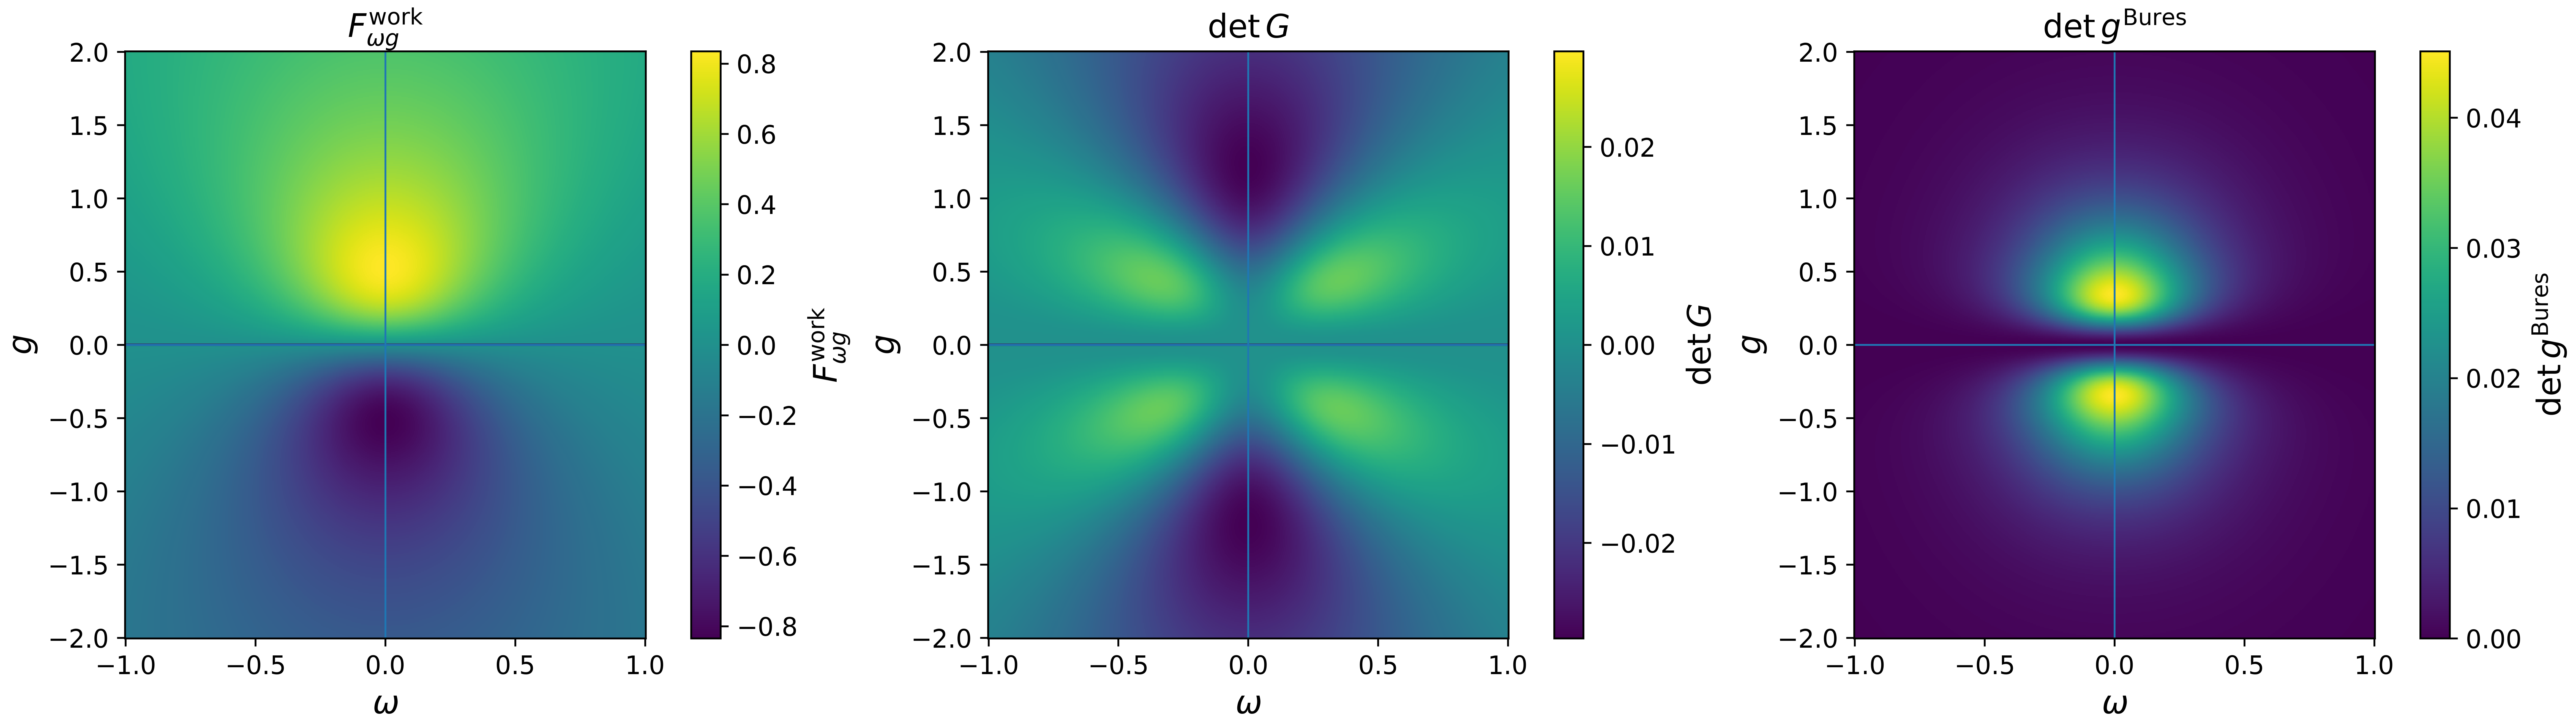
\includegraphics[width=\textwidth]{Figures/Figure1_F_vs_G_vs_g.png}
\caption{
\textbf{Comparison of response geometry and information geometry for a driven open quantum system.}
The three panels display complementary geometric structures
defined over the same two-dimensional control manifold
parameterized by the Hamiltonian frequency $\omega$ and coherent
coupling strength $g$. All quantities are computed from the same
family of nonequilibrium stationary density operators of the
driven qubit model.
(a) Antisymmetric work curvature
$F_{\omega g}^{\rm work}$.
This field governs the geometric contribution to quasistatic
cyclic work and changes sign under reversal of the orientation of
the control cycle. The nodal line separates regions of opposite
geometric orientation and is analogous to the curvature fields
introduced earlier for equilibrium thermodynamic systems.
(b) Determinant of the symmetric response metric,
$\det G$.
This quantity measures the magnitude of the reciprocal component
of the local response tensor and characterizes the local
susceptibility of the nonequilibrium steady state to changes in
the external control parameters. Unlike the antisymmetric
curvature, the response metric is insensitive to the orientation
of parameter-space loops.
(c) Determinant of the Bures metric,
$\det g^{\rm Bures}$.
The Bures metric is an information-geometric measure of the
distinguishability of neighboring stationary density operators
and is proportional to the quantum Fisher information. It
contains no antisymmetric component and therefore cannot describe
geometric work or nonreciprocal response.
Although all three fields are generated from the same family of
stationary states, they exhibit markedly different spatial
organization. The work curvature possesses a signed dipolar
structure associated with nonreciprocal response, the response
metric develops a quadrupolar pattern characteristic of
reciprocal susceptibility, and the Bures metric is localized near
the avoided crossing where neighboring stationary states become
most rapidly distinguishable. Their coexistence demonstrates that
nonequilibrium quantum systems possess multiple, complementary
geometric structures. Response geometry and information geometry
are therefore related through the common stationary-state
manifold, but they encode fundamentally different physical
properties.
}
\label{fig:F_G_Bures}
\end{figure*}

Figure~\ref{fig:F_G_Bures} compares these geometric structures
for the driven qubit introduced in the previous subsection.
Panel (a) shows the antisymmetric work curvature
$F_{\omega g}^{\rm work}$, panel (b) the determinant of the
symmetric response metric $G$, and panel (c) the determinant of
the Bures metric. All three quantities are evaluated on the same
control manifold and are generated from the same family of
nonequilibrium steady states.
Several observations immediately emerge. First, the
antisymmetric work curvature possesses a signed dipolar
structure reflecting the orientation dependence of quasistatic
cycles. Second, the response metric exhibits a quadrupolar
organization associated with reciprocal susceptibility. Finally,
the Bures metric is concentrated near the avoided crossing,
where neighboring stationary states become most rapidly
distinguishable. Although all three fields derive from the same
steady-state manifold, they emphasize fundamentally different
aspects of the response.
This comparison demonstrates that response geometry and
information geometry are complementary rather than equivalent.
The response metric characterizes how physical observables change
under external driving, whereas the Bures metric characterizes
how rapidly the quantum state itself changes. Agreement between
the two is therefore neither expected nor required. Instead,
their differences provide additional physical information about
the relationship between dynamical response and state-space
structure.
This distinction motivates the introduction of an enlarged
response tensor whose Hermitian structure naturally contains both
the reciprocal response metric and the antisymmetric work
curvature. Information geometry then appears not as a
replacement for response geometry, but as an independent metric
structure defined on the same manifold of stationary states.




\subsection{Complementarity and the Triality Manifold}
The Bloch representation introduced in the preceding
subsection provides a convenient description of the
stationary state of a driven qubit. While the Cartesian
coordinates $(x,y,z)$ completely specify the reduced
density operator, they do not directly distinguish the
different physical resources that characterize an open
quantum system. It is therefore useful to introduce a
coordinate system whose components possess immediate
physical interpretation.

For a stationary Bloch vector
\begin{align}
\mathbf{r}
=
(x,y,z),
\end{align}
we define the coherence
\begin{align}
C
=
\sqrt{x^2+y^2},
\end{align}
which measures the magnitude of the off-diagonal
coherence within the pointer-basis plane, together with
the predictability
\begin{align}
P
=
z,
\end{align}
which measures the population imbalance between the
pointer states. The Bloch-vector magnitude is
\begin{align}
R
=
\sqrt{x^2+y^2+z^2},
\end{align}
with $R\le1$, where equality holds only for pure states.

The departure from the Bloch-sphere surface is measured
by the openness coordinate
\begin{align}
E
=
\sqrt{1-R^2},
\end{align}
which quantifies the contraction of the Bloch sphere
resulting from environmental mixing and reduction from
the larger system--environment Hilbert space.

These variables satisfy the normalized triality relation
\begin{align}
C^2+P^2+E^2=1,
\label{eq:triality}
\end{align}
which defines a quarter-sphere manifold containing all
physically admissible reduced steady states. In this
representation, coherence and predictability specify the
cylindrical projection of the Bloch vector, while
openness appears naturally as a radial deficit. Pure
states lie on the boundary $E=0$, whereas increasing
interaction with the environment moves the system
toward the interior of the manifold.

\begin{figure*}[t]
\centering
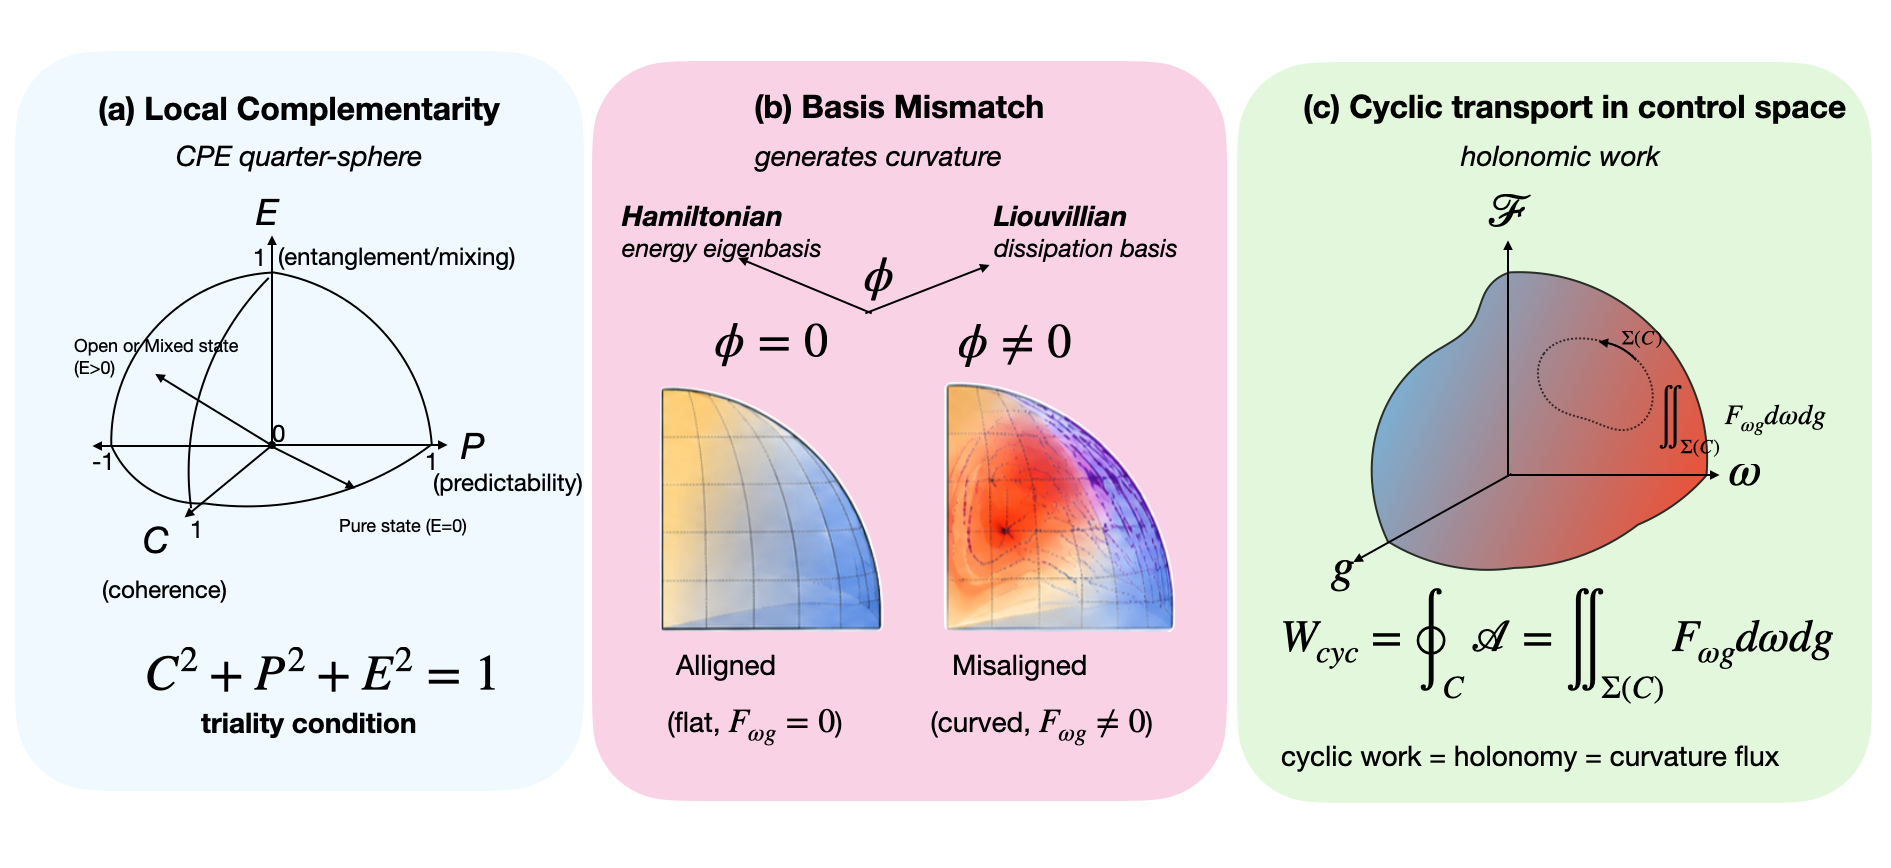
\includegraphics[width=\textwidth]{Figures/CPE_Fig0.png}
\caption{
\textbf{Complementarity and the triality manifold for open quantum systems.}
(a) The complementarity variables coherence $C$,
predictability $P$, and openness $E$ provide a natural
coordinate system for the reduced steady-state manifold of
a driven qubit. These variables satisfy the normalized
triality relation
$C^{2}+P^{2}+E^{2}=1$,
so that every physically admissible reduced state occupies
a point on the quarter sphere. Coherence measures the
off-diagonal quantum superposition within the pointer-basis
plane, predictability measures the population imbalance,
and openness quantifies the contraction of the Bloch sphere
resulting from environmental mixing.
(b) Schematic illustration of the competition between
coherent Hamiltonian evolution and environmentally selected
pointer states. When the Hamiltonian and pointer bases are
aligned, the stationary state reduces to the Gibbs manifold
and the response is integrable. Misalignment between these
structures produces genuinely nonequilibrium steady states
whose response cannot, in general, be derived from a global
thermodynamic potential.
(c) Conceptual representation of quasistatic transport over
the control manifold. Cyclic evolution generates a geometric
response that depends upon the path taken through parameter
space rather than only the initial and final states. The
formal relationship between the local response tensor, the
antisymmetric response field, and the resulting cyclic work
is developed in the following sections.
Throughout this review, the triality manifold serves as the
canonical state-space representation for open quantum
systems. The complementarity variables $(C,P,E)$ specify
the local steady state, while subsequent figures paint
response fields onto this manifold to illustrate the
relationship between complementarity, nonequilibrium
response, geometric transport, and observational
reconstruction.
}
\label{fig:CPE}
\end{figure*}

Figure~\ref{fig:CPE} summarizes this geometric
construction. Panel (a) illustrates the triality
manifold defined by Eq.~(\ref{eq:triality}), where every
point corresponds to a physically admissible reduced
steady state. The variables $(C,P,E)$ therefore provide
a physically motivated coordinate system whose axes
represent coherence, predictability, and openness,
respectively, rather than Cartesian components of the
Bloch vector.


The remaining panels anticipate the geometric structure
developed in the following sections. Panel (b)
illustrates how complementarity between coherent
Hamiltonian evolution and environmentally selected
pointer states generates nontrivial response on the
triality manifold, while panel (c) depicts the cyclic
transport associated with quasistatic evolution over the
control manifold. At this stage these panels should be
viewed primarily as a roadmap for the subsequent
development. Their physical interpretation in terms of
response geometry, antisymmetric response, and
holonomic transport will be developed after the local
response tensor has been introduced.

Within the framework developed in this review, the
triality manifold plays a role analogous to the
thermodynamic state space of equilibrium statistical
mechanics. The variables $(C,P,E)$ specify the local
state of the reduced quantum system, whereas the
response tensor introduced in the following subsection
determines how that state changes under infinitesimal
variations of the external control parameters. The
triality variables therefore answer the question
\emph{where is the system on the steady-state manifold?},
while the response geometry answers the complementary
question \emph{how does that state respond to external
driving?}

This distinction provides a unifying perspective for the
remainder of the review. The complementarity variables
define the local coordinate structure of the
nonequilibrium steady-state manifold, while the response
geometry endows that manifold with reciprocal and
nonreciprocal response fields. Subsequent sections will
show that these local fields govern quasistatic
transport, geometric work, and the observational
reconstruction of nonequilibrium quantum response.


\section{Observational Geometry: Reconstructing Response from Experiment}
\label{sec:observational}
The preceding sections developed the intrinsic geometry of
nonequilibrium response. Beginning with quasistatic evolution on
the Liouvillian control manifold, we showed that open quantum
systems possess a natural geometric structure defined by a work
one-form, its associated curvature, and a local response tensor
whose symmetric and antisymmetric components describe reciprocal
and nonreciprocal response. These objects are intrinsic
properties of the stationary-state manifold. Like the metric and
curvature tensors of differential geometry, they exist
independently of any particular experimental realization.
Physical measurements, however, do not access these intrinsic
geometric quantities directly. Spectroscopic experiments probe
transition amplitudes, optical coherences, and time-dependent
polarization, whereas the response metric and curvature are
properties of the parameter-dependent Liouvillian governing the
underlying dynamics. The central challenge is therefore one of
geometric reconstruction: how may the intrinsic geometry of the
response manifold be inferred from experimentally observable
signals?

The answer developed in our recent work is to reinterpret
nonlinear spectroscopy as a problem in geometric transport.
Conventional response theory expands the density operator in
powers of the external optical field while holding the
Liouvillian fixed. This approach successfully describes the
generation of nonlinear optical signals but implicitly assumes
that the generator of the dynamics is known exactly. In practice,
however, microscopic models are necessarily approximate.
Important physical processes---including environmental
fluctuations, correlated dissipation, spin-orbit coupling,
vibronic interactions, and collective many-body effects---are
often neglected in an initial description and subsequently
introduced through increasingly sophisticated Hamiltonians or
system--bath models.

From the perspective of response geometry, these additional
physical interactions should not be viewed merely as corrections
to the calculated spectrum. Rather, they modify the generator of
the dynamics itself and therefore alter the geometry of the
underlying response manifold. Improving the microscopic model is
thus equivalent to refining the geometric description of the
system. The experimentally observed spectrum changes because the
local response geometry has changed.

This observation suggests a natural extension of conventional
perturbation theory. Instead of expanding only the interaction
with the optical field, we regard the Liouvillian itself as a
parameter-dependent object,
\begin{align}
\mathcal L
=
\mathcal L(\lambda),
\end{align}
where the control coordinates
$\lambda=(\lambda^1,\lambda^2,\ldots)$
may represent external fields, temperatures, system--bath
couplings, or other experimentally tunable parameters. Motion
through this control manifold induces corresponding changes in
the generator of the dynamics,
\begin{align}
\mathcal L(\lambda+\delta\lambda)
=
\mathcal L(\lambda)
+
\delta\lambda^\mu
\partial_\mu\mathcal L
+
\frac12
\delta\lambda^\mu
\delta\lambda^\nu
\partial_\mu\partial_\nu\mathcal L
+\cdots.
\end{align}
The problem therefore becomes one of transporting observables
through a continuously varying family of Liouvillian generators.
This shift in perspective represents the principal conceptual
advance of the observational framework. Conventional nonlinear
spectroscopy reconstructs dynamical response by perturbatively
expanding the interaction with the radiation field. Here the
perturbation parameter is instead the motion of the Liouvillian
through the response manifold itself. The resulting Duhamel
expansion naturally defines transport operators that connect
observable spectroscopic signals with the intrinsic metric and
curvature developed in the preceding sections. In this way,
response geometry becomes experimentally accessible, completing
the progression from intrinsic geometry to observable geometry.


\begin{tcolorbox}[
colback=gray!5,
colframe=black,
title=\textbf{Principle of Geometric Refinement},
fonttitle=\bfseries,
breakable]
\textbf{Microscopic model refinement is equivalent to geometric refinement.}
Traditional spectroscopy systematically improves microscopic
Hamiltonians or system--bath models until the calculated spectra
reproduce experiment. Within the framework developed here, this
process admits a complementary geometric interpretation. Each
additional physical interaction modifies the Liouvillian
generator and therefore deforms the local response geometry.
The experimentally observed spectrum changes because the
underlying response manifold has been refined.
The Duhamel expansion provides the differential calculus
governing this geometric refinement. Rather than simply adding
perturbative corrections to the dynamics, it describes how the
response metric, curvature, and observable transport evolve as
the microscopic description becomes progressively more complete.
From this perspective, nonlinear spectroscopy is no longer
viewed primarily as a method for determining Hamiltonian
parameters, but as a means of reconstructing and refining the
geometry of physical response.
\end{tcolorbox}

\subsection{Differential Geometry of Liouville Space}
\label{subsec:liouville_geometry}
The preceding sections established the intrinsic geometry of
thermodynamic response. Metrics and curvature characterize the
response of stationary states to variations of external control
parameters and determine the local and global structure of
nonequilibrium thermodynamics. Spectroscopic measurements,
however, do not probe stationary states directly. They interrogate
the dynamical evolution of optical coherences and populations,
requiring a geometric description of transport on the manifold of
Liouvillian generators rather than on the manifold of stationary
states alone.

This distinction is fundamental. The response curvature
$F_{\mu\nu}$ introduced earlier governs quasistatic work and
nonreciprocal thermodynamic response. Spectroscopy instead probes
how dynamical pathways evolve as the generator of the dynamics is
varied. The relevant geometric objects are therefore connections
and curvature defined on the Liouvillian manifold itself.

\subsubsection{Transport of Liouvillian Eigenoperators}
Consider a parameter-dependent Liouvillian
\begin{align}
\mathcal L=\mathcal L(\lambda),
\end{align}
where the control coordinates
$\lambda^\mu=(\lambda^1,\lambda^2,\ldots)$
may represent thermodynamic variables, external fields,
pulse-sequence parameters, system--bath couplings, or other
experimentally tunable quantities. The corresponding
Liouvillian eigenproblem is
\begin{align}
\mathcal L(\lambda)\Phi_n(\lambda)
=
\Lambda_n(\lambda)\Phi_n(\lambda),
\end{align}
together with the biorthogonal left eigenoperators
\begin{align}
\widetilde\Phi_m^\dagger(\lambda)
\mathcal L(\lambda)
=
\Lambda_m(\lambda)
\widetilde\Phi_m^\dagger(\lambda),
\end{align}
normalized according to
\begin{align}
\langle\!\langle
\widetilde\Phi_m
|
\Phi_n
\rangle\!\rangle
=
\delta_{mn}.
\end{align}
As the control parameters vary, both the eigenvalues and the
eigenoperators evolve. These two forms of variation have
fundamentally different physical consequences.
Changes in the eigenvalues modify oscillation frequencies,
relaxation rates, and dephasing times, but do not alter the
underlying organization of spectroscopic pathways. By contrast,
changes in the eigenoperators modify the Liouville-space basis
itself, transporting populations and coherences between
pathways. Geometry therefore resides not in the evolution of the
Liouvillian spectrum, but in the evolution of its eigenoperators.

A simple example is provided by pure dephasing. The decoherence
rate may depend strongly upon temperature while the
eigenoperators remain fixed. In that case the spectrum changes,
yet no geometric pathway transport occurs. Nontrivial geometric
response emerges only when the eigenoperators themselves evolve
with the control parameters.

\begin{tcolorbox}[
colback=gray!5,
colframe=black,
title=\textbf{Principle of Pathway Geometry},
fonttitle=\bfseries]
Geometric transport is governed by the evolution of
Liouvillian eigenoperators, not by the evolution of
Liouvillian eigenvalues. Eigenvalues determine rates;
eigenoperators determine geometry.
\end{tcolorbox}

\subsubsection{Liouvillian Connections}
Comparing pathway bases defined at neighboring points of the
control manifold requires a rule for parallel transport. The
appropriate object is the Liouvillian connection,
\begin{align}
\Gamma_\mu
=
\partial_\mu\mathcal L,
\end{align}
which measures the local deformation of the generator under an
infinitesimal displacement in parameter space.
Expressed in the local Liouvillian eigenbasis,
\begin{align}
(\Gamma_\mu)_{mn}
=
\langle\!\langle
\widetilde\Phi_m
|
\Gamma_\mu
|
\Phi_n
\rangle\!\rangle,
\end{align}
the diagonal elements describe the response of individual
pathways, while the off-diagonal elements couple distinct
pathways and generate transport throughout the Liouville-space
network.

The Liouvillian connection plays a role analogous to the Berry
connection for adiabatic quantum evolution. The difference is
that the transported objects are not wavefunctions but
Liouvillian eigenoperators and the spectroscopic pathways they
define. Consequently, Liouvillian geometry naturally incorporates
dissipation, decoherence, and environmental interactions, all of
which lie outside conventional Berry theory.
\subsubsection{Curvature and Pathway Transport}
Transport generated by different physical mechanisms generally
does not commute. Coherent evolution, dissipation,
system--bath interactions, and optical driving define competing
transport directions in Liouville space,
\begin{align}
\mathcal L
=
\mathcal L_H
+
\mathcal L_D
+
\mathcal L_{\rm int}
+\cdots,
\end{align}
with
\begin{align}
[
\mathcal L_\alpha,
\mathcal L_\beta
]
\neq0.
\end{align}
The incompatibility of these transport directions is quantified
by the Liouvillian curvature,
\begin{align}
\mathcal K_{\mu\nu}
=
\partial_\mu\Gamma_\nu
-
\partial_\nu\Gamma_\mu
+
[
\Gamma_\mu,\Gamma_\nu
].
\end{align}
This curvature measures the failure of successive transport
operations to commute and therefore quantifies the intrinsic
geometry of pathway transport.

Transport around a closed loop generates the Liouvillian
holonomy,
\begin{align}
\mathcal U_C
=
\mathcal P
\exp
\left[
\oint_C
\Gamma_\mu
d\lambda^\mu
\right],
\end{align}
which represents the cumulative geometric transformation of the
pathway basis.

\subsubsection{Observable Bundles and Observational Holonomy}
The full Liouville-space transport is not directly accessible to
experiment. Spectroscopy measures
\begin{align}
S(t)
=
{\rm Tr}
[
O\rho(t)
],
\end{align}
where the observable $O$ projects the evolving density operator
onto a particular measurement channel. Every spectroscopic
experiment therefore defines an induced observable bundle obtained
by projecting the intrinsic Liouville bundle onto the subspace
selected by the preparation and detection operators.
The experimentally observed transport is consequently not the
full Liouvillian holonomy but its projection onto this observable
bundle. We refer to this projected quantity as the
\emph{observational holonomy}. Different observables probe
different projections of the same underlying Liouvillian
transport and therefore need not reveal identical geometric
structure
.
Observation is therefore itself a geometric operation. The
measured spectrum resides not on the intrinsic Liouvillian
manifold but on an observable manifold induced by the
measurement process. Reconstructing response geometry from
spectroscopy is therefore simultaneously a problem of dynamical
transport and observable projection.

\subsubsection{Geometric Refinement}
The differential geometry developed above provides the intrinsic
description of Liouville-space transport. The remaining question
is computational: given an approximate Liouvillian, how does one
systematically refine its geometry until the predicted
observational holonomy agrees with experiment?

Within the present framework, improving a microscopic model is
equivalent to refining its response geometry. Each additional
physical interaction modifies the Liouvillian connection and
curvature, thereby deforming the local geometry of pathway
transport. The Duhamel expansion introduced in the following
section provides the differential calculus governing this process
of geometric refinement.


%at end
\begin{tcolorbox}[
colback=gray!5,
colframe=black,
title=\textbf{Principle of Observational Holonomy},
fonttitle=\bfseries,
breakable]
The Liouvillian connection defines the transport of dynamical
pathways on the manifold of generators. Spectroscopic
measurements, however, do not observe this transport directly.
Instead, they measure only its projection onto the observable
subspace selected by the preparation and detection operators.
Consequently, the experimentally reconstructed holonomy is not
the full Liouville-space holonomy, but the holonomy induced on
the observable subspace. Observation is therefore a geometric
projection, and different spectroscopic protocols reconstruct
different projections of the same underlying response geometry.
The basis-misalignment angle $\theta$ is the local coordinate
parameterizing this observable projection. Reconstructing
$\theta$ from nonlinear spectra is therefore equivalent to
reconstructing the local observational geometry.
\end{tcolorbox}




\subsection{The Canonical Two-Level Coordinate Chart}
\label{subsec:canonical2LS}
The differential geometry developed in the preceding section is
completely general and applies to arbitrary open quantum systems.
To expose its essential structure, however, it is useful to
introduce the simplest nontrivial realization of observational
geometry. Rather than viewing the two-level system as a minimal
model, we regard it as the canonical local coordinate chart on
the manifold of Liouvillian geometries.

The privileged role of the two-level system in quantum mechanics
extends naturally to observational geometry. Just as the tangent
plane provides a local coordinate chart for a differentiable
manifold, the canonical two-level system provides the simplest
local coordinate chart for the manifold of Liouvillian
geometries. Although realistic open quantum systems generally
possess high-dimensional response manifolds with many interacting
pathways, their local geometric structure is frequently governed
by the effective coupling of a pair of pathways. The single
observational coordinate $\theta$ therefore captures the leading
local deformation of the observable bundle in precisely the same
way that local coordinates describe the neighborhood of a point
on a manifold. Higher-dimensional systems require additional
geometric coordinates, but the underlying notions of Liouvillian
connection, curvature, pathway transport, and observational
holonomy remain unchanged. The canonical two-level system should
therefore be viewed not as a special physical model, but as the
\textit{universal local chart from which the differential geometry of
observational response is constructed.}

The same canonical two-level system has appeared throughout the
development of the present framework. In our earlier work on
stationary-state response, it provided the simplest realization
of response geometry, illustrating how the misalignment between
the Hamiltonian and pointer bases generates a symmetric response
metric together with an antisymmetric curvature two-form. Here,
the physical model remains unchanged, but the question is
different. Rather than asking how this geometry determines
quasistatic work performed around a closed control cycle, we ask
how it manifests itself in nonlinear optical measurements.

Observation therefore introduces an additional geometric layer:
the transport of observable pathways through Liouville space.
The canonical model consists of a two-level Hamiltonian,
\begin{align}
H=\frac{\Delta}{2}\sigma_z,
\end{align}
whose eigenstates define the observational basis used by the
spectroscopic experiment. In the absence of environmental
coupling, these states generate the familiar independent
Liouville-space pathways that underlie the conventional
decomposition of the nonlinear response.
The environment, however, selects its own preferred pointer
basis, related to the observational basis through the unitary
transformation
\begin{align}
|p_n\rangle
=
U(\theta)
|e_n\rangle,
\end{align}
where $\theta$ is the local coordinate of the canonical
observable chart. Physically, $\theta$ is realized as the
misalignment between the observational basis defined by the
experiment and the pointer basis selected by the environment.
Geometrically, however, it is more fundamental: it parameterizes
the local deformation of the observable bundle induced by
environmental interactions.

When $\theta=0$, the observational and pointer bases coincide.
The dissipative dynamics reduce to pure dephasing in the
observational basis, Liouville-space pathways remain independent,
and no observational transport is generated. As $\theta$
increases, environmental monitoring mixes populations and
coherences, activating transport between pathways and generating
the observational geometry described in the previous section.
Recovering $\theta$ from nonlinear spectroscopic measurements is
therefore equivalent to reconstructing the leading local
deformation of the observable bundle.
The two-level system is therefore not important because it is
simple, but because it exposes the local differential geometry in
its most transparent form. More complex systems require
additional coordinates and a corresponding atlas of overlapping
coordinate charts, yet the underlying geometric construction
remains unchanged. The canonical two-level chart thus plays the
same role in observational geometry that the tangent plane plays
in differential geometry: it provides the universal local model
from which the global geometry is assembled.




\subsection{Liouville Propagator Expansion and the Transport Matrix}
\label{subsec:duhamel_transport}
The canonical two-level chart identifies the local observational
coordinate \(\theta\), but it does not by itself determine how
spectroscopic pathways are transported. To compute that transport
we require a perturbative expansion of the Liouville propagator.
This is the point at which the Duhamel expansion enters: not as
the starting point of the theory, but as the calculational
machinery for refining the local Liouvillian geometry.

Let the Liouvillian depend smoothly on a set of local deformation
coordinates \(\lambda^\mu\). Near a reference Liouvillian
\(\mathcal L_0=\mathcal L(\lambda=0)\), we write
\begin{align}
\mathcal L(\lambda)
=
\mathcal L_0
+
\lambda^\mu \mathcal X_\mu
+
\frac12
\lambda^\mu\lambda^\nu
\mathcal Y_{\mu\nu}
+
O(\lambda^3),
\label{eq:L_local_expansion}
\end{align}
where
\begin{align}
\mathcal X_\mu
&=
\left.
\partial_\mu\mathcal L
\right|_{\lambda=0},
&
\mathcal Y_{\mu\nu}
&=
\left.
\partial_\mu\partial_\nu\mathcal L
\right|_{\lambda=0}.
\end{align}
The operators \(\mathcal X_\mu\) are tangent vectors on the
manifold of Liouvillian geometries. They identify the leading
directions in which the generator is deformed away from the
reference dynamics. The tensors \(\mathcal Y_{\mu\nu}\) describe
the local nonlinear deformation of this manifold. In the canonical
two-level chart the coordinate manifold is one-dimensional and
\(\lambda^\mu\rightarrow\theta\), so that
\begin{align}
\mathcal L(\theta)
=
\mathcal L_0
+
\theta\mathcal X
+
\frac{\theta^2}{2}\mathcal Y
+
O(\theta^3).
\label{eq:L_theta_expansion_review}
\end{align}
The propagator over a waiting interval \(\tau\) is
\begin{align}
U(\tau;\lambda)
=
\exp\left[
\mathcal L(\lambda)\tau
\right].
\end{align}
Because \(\mathcal L_0\) and the deformation operators generally
do not commute, the exponential cannot be expanded as an ordinary
scalar Taylor series. The appropriate expansion is the Duhamel
series, which expresses the perturbed propagator as insertions of
the deformation operators into the reference evolution. To second
order,
\begin{align}
U(\tau;\lambda)
=
U_0(\tau)
+
\lambda^\mu U^{(1)}_\mu(\tau)
+
\frac12
\lambda^\mu\lambda^\nu
U^{(2)}_{\mu\nu}(\tau)
+
O(\lambda^3),
\label{eq:U_duhamel_review}
\end{align}
with
\begin{align}
U_0(\tau)
=
e^{\mathcal L_0\tau},
\end{align}
and
\begin{align}
U^{(1)}_\mu(\tau)
=
\int_0^\tau ds\,
e^{\mathcal L_0(\tau-s)}
\mathcal X_\mu
e^{\mathcal L_0 s}.
\label{eq:U1_duhamel_review}
\end{align}
The first-order term describes a single deformation event inserted
at time \(s\), propagated before and after by the reference
Liouvillian.

The second-order contribution contains two distinct pieces:
\begin{align}
U^{(2)}_{\mu\nu}(\tau)
&=
\int_0^\tau ds\,
e^{\mathcal L_0(\tau-s)}
\mathcal Y_{\mu\nu}
e^{\mathcal L_0 s}
\nonumber\\
&\quad
+
2
\int_0^\tau ds
\int_0^s ds'\,
e^{\mathcal L_0(\tau-s)}
\mathcal X_\mu
e^{\mathcal L_0(s-s')}
\mathcal X_\nu
e^{\mathcal L_0s'} .
\label{eq:U2_duhamel_review}
\end{align}
The first term is a single insertion of the second-order
deformation \(\mathcal Y_{\mu\nu}\). The second is a double
insertion of the first-order tangent operators
\(\mathcal X_\mu\) and \(\mathcal X_\nu\), separated by free
evolution under \(\mathcal L_0\). This term is the explicit
Liouville-space expression of pathway transport generated by
successive noncommuting deformations.

To connect this propagator expansion to spectroscopy, let
\(\{S_a^{(0)}\}\) denote the conventional zeroth-order pathway
decomposition of the nonlinear signal,
\begin{align}
S^{(0)}
=
\sum_a S_a^{(0)} .
\end{align}
In the reference geometry each pathway evolves independently. A
deformation of the Liouvillian transports amplitude among these
pathways, so that the observed pathway amplitudes may be written
as
\begin{align}
S_a(\lambda)
=
\sum_b
T_{ab}(\lambda)
S_b^{(0)} .
\label{eq:pathway_transport_review}
\end{align}
The matrix \(T_{ab}\) is the observable transport matrix. It is
the representation of Liouville-space transport on the
experimentally accessible pathway basis. Its diagonal elements
renormalize individual pathway weights, while its off-diagonal
elements quantify transfer of amplitude between pathways.

Projecting the Duhamel-expanded propagator onto the zeroth-order
pathway basis gives
\begin{align}
T_{ab}(\lambda)
=
\delta_{ab}
+
\lambda^\mu T^{(1)}_{ab,\mu}
+
\frac12
\lambda^\mu\lambda^\nu
T^{(2)}_{ab,\mu\nu}
+
O(\lambda^3).
\label{eq:T_expansion_review}
\end{align}
The coefficients \(T^{(1)}_{ab,\mu}\) are obtained by inserting
\(U^{(1)}_\mu\) into the corresponding Liouville pathway
expression, while \(T^{(2)}_{ab,\mu\nu}\) are obtained from
\(U^{(2)}_{\mu\nu}\). Thus the transport matrix is not an
independent phenomenological fitting object. It is the projected
representation of the local Liouvillian deformation on the
observable bundle.

For the canonical two-level chart this reduces to
\begin{align}
T_{ab}(\theta)
=
\delta_{ab}
+
\theta T^{(1)}_{ab}
+
\frac{\theta^2}{2}
T^{(2)}_{ab}
+
O(\theta^3).
\label{eq:T_theta_review}
\end{align}
The experimentally reconstructed parameter \(\theta\) is therefore
not merely a basis-misalignment angle. It is the local coordinate
that determines how the observable pathway basis is transported
away from the reference geometry. Reconstructing \(\theta\) from
nonlinear spectra is equivalent to reconstructing the leading
deformation of the observable bundle.

It is useful to distinguish the Taylor coefficients
\(\mathcal Y_{\mu\nu}\) from the Liouvillian curvature
\(\mathcal K_{\mu\nu}\). The former describe local nonlinear
changes of the generator in a chosen coordinate chart. The latter
is constructed from the Liouvillian connection and measures the
failure of transport operations to commute:
\begin{align}
\mathcal K_{\mu\nu}
=
\partial_\mu\Gamma_\nu
-
\partial_\nu\Gamma_\mu
+
[\Gamma_\mu,\Gamma_\nu].
\end{align}
Both arise from the same underlying Liouvillian geometry, but
they encode different information. The tensors
\(\mathcal Y_{\mu\nu}\) describe the local shape of the generator
manifold, while \(\mathcal K_{\mu\nu}\) describes the curvature
of transport on that manifold.

Equations~\eqref{eq:U_duhamel_review}--\eqref{eq:T_theta_review}
give the operational form of geometric refinement. Beginning from
a reference Liouvillian, additional physical interactions deform
the generator, transport amplitude among observable pathways, and
alter the measured nonlinear spectrum. The Duhamel expansion is
therefore not simply a perturbative correction to the signal. It
is the differential calculus by which the local response geometry
is refined and projected into experimentally measurable form.

\subsection{Liouville Pathways as an Observable Basis}
\label{subsec:pathway_basis}
Nonlinear optical spectroscopy is traditionally formulated as a
sum over Liouville-space pathways, each represented by a
double-sided Feynman diagram specifying a particular sequence of
light--matter interactions and free evolution. The third-order
polarization may be written schematically as
%
\begin{align}
P^{(3)}(t)
=
\sum_a
S_a(t),
\label{eq:P3sum}
\end{align}
%
where the index $a$ labels every Liouville pathway contributing
to the measured signal. Depending upon the system under
consideration, these include rephasing and non-rephasing
contributions arising from ground-state bleach (GSB), stimulated
emission (SE), excited-state absorption (ESA), double-quantum
coherences, and higher-order processes. The experimentally
observed spectrum is obtained only after coherent summation over
all contributing pathways.
Conventionally, the individual Liouville pathways are regarded as
diagrammatic bookkeeping devices that organize the perturbation
expansion of the nonlinear response. Within the present
framework, however, they admit a deeper geometric
interpretation. The collection of pathway amplitudes
%
\begin{align}
\mathbf{S}
=
\left(
S_1,
S_2,
\ldots,
S_N
\right)^T
\end{align}
%
forms a natural basis for the observable bundle associated with
the chosen experiment. The individual Liouville pathways are
therefore not merely contributions to the spectrum, but basis
vectors spanning the space of experimentally accessible
responses.

The geometric role of the Liouvillian is to transport this basis
through the manifold of response geometries. As the Liouvillian
is deformed by changes in the system Hamiltonian, environmental
couplings, external fields, or thermodynamic conditions, pathway
amplitudes are redistributed throughout the observable basis.
The response is therefore no longer described by independent
Liouville pathways, but by a transported basis,
%
\begin{align}
S_a
=
\sum_b
T_{ab}
S_b^{(0)},
\label{eq:Ttransport}
\end{align}
%
where $S_b^{(0)}$ denotes the reference pathway amplitudes and
$T_{ab}$ is the observable transport operator. The operator
itself is intrinsic to the Liouvillian geometry, while the matrix
elements shown above are its representation in the chosen
Liouville-pathway basis. The diagonal elements describe the
renormalization of individual pathway amplitudes, whereas the
off-diagonal elements quantify transport between distinct
Liouville pathways generated by the environment.

For the canonical two-level coordinate chart introduced in the
previous section, the observable basis is particularly compact.
The third-order response contains only the GSB and ESA
contributions, each possessing both rephasing and non-rephasing
sectors, so that the complete signal is obtained by summing over
all transported Liouville pathways. The resulting transport
operator is therefore of low dimension, making the underlying
geometry especially transparent. In realistic molecular and
condensed-phase systems, the observable bundle expands to include
many additional pathways, but the geometric construction remains
unchanged. The transport operator continues to describe the
evolution of the complete Liouville-pathway basis; only the
dimension of the observable bundle increases.

This interpretation establishes a direct correspondence between
the differential geometry developed in the preceding sections and
the familiar diagrammatic language of nonlinear spectroscopy.
Liouville pathways play the role of local basis vectors for the
observable bundle, the Liouvillian connection specifies their
infinitesimal transport, the curvature measures the
noncommutativity of successive transport operations, and the
observed nonlinear spectrum is the projection of the transported
basis onto the experimental detection channel. From this
perspective, nonlinear spectroscopy is naturally reinterpreted as
a measurement of the transport of an observable basis through the
manifold of Liouvillian geometries.


\section{Numerical Demonstration of Geometric Reconstruction}
\label{sec:numerics}
The preceding sections established the theoretical framework
underlying observational geometry. The remaining question is
whether the local geometric coordinates can, in practice, be
reconstructed from nonlinear spectroscopic data. We now
illustrate this reconstruction using the canonical two-level
coordinate chart developed above. Although deliberately simple,
this model contains all of the essential ingredients of the
geometric theory while permitting direct comparison between exact
Liouvillian propagation and the Duhamel transport expansion.

\begin{figure*}
\centering
\begin{minipage}{0.48\textwidth}
\centering
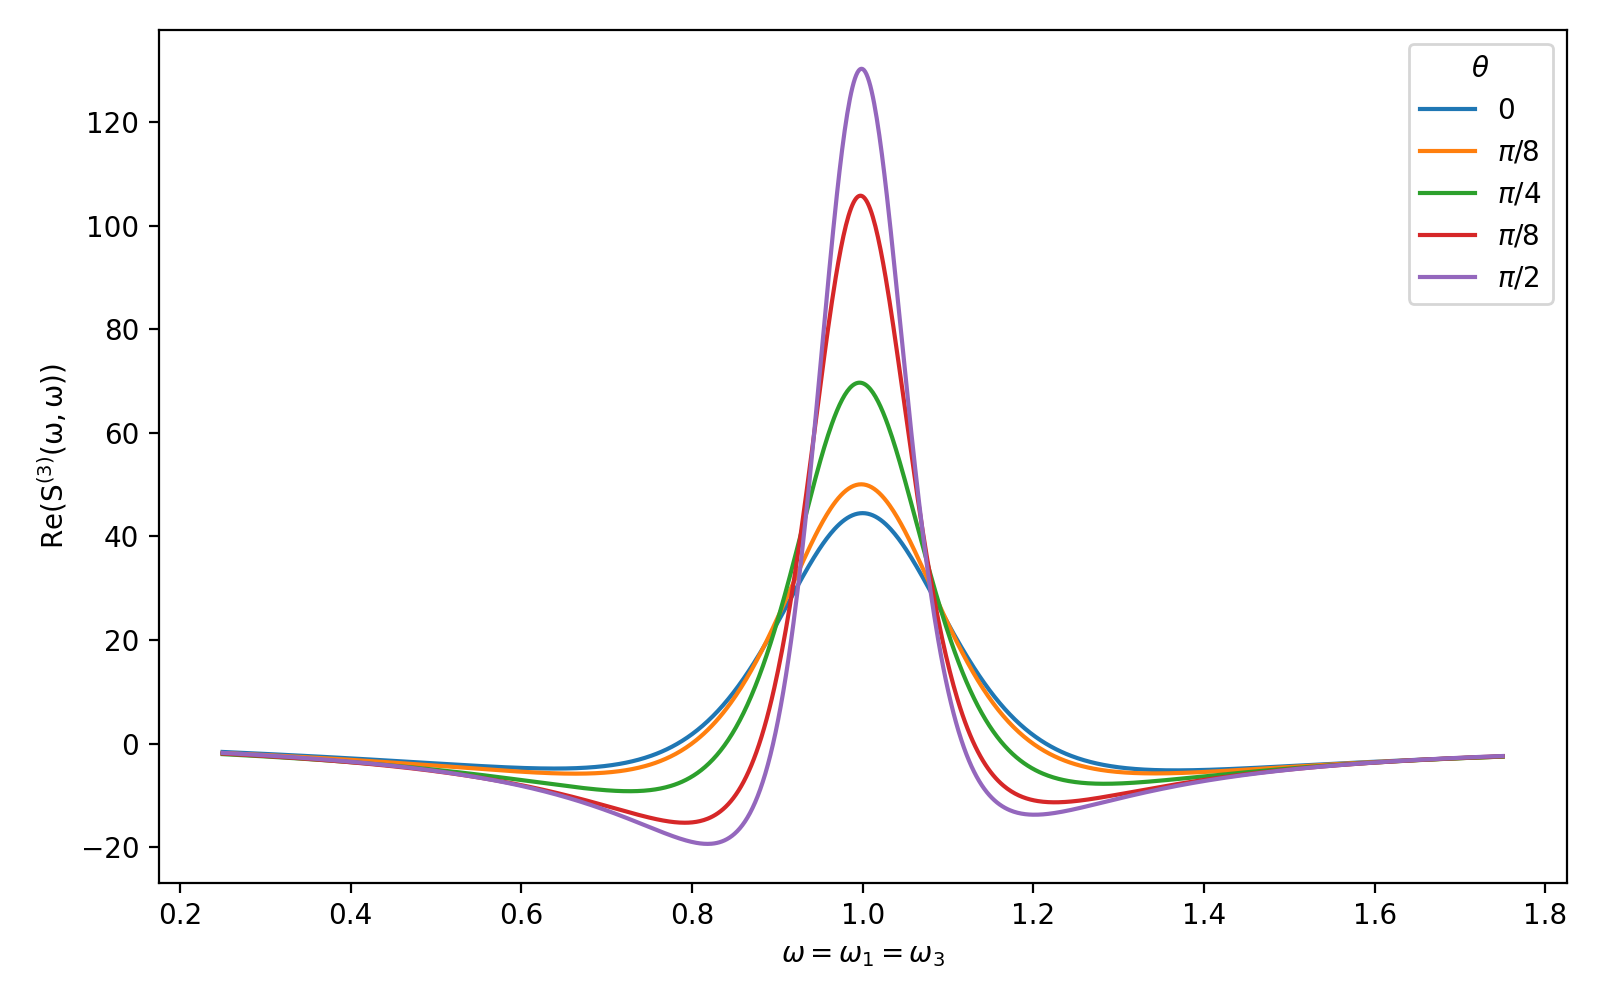
\includegraphics[width=\linewidth]{Figures/corrected_diag_theta_real_2.png}
\end{minipage}
\hfill
\begin{minipage}{0.48\textwidth}
\centering
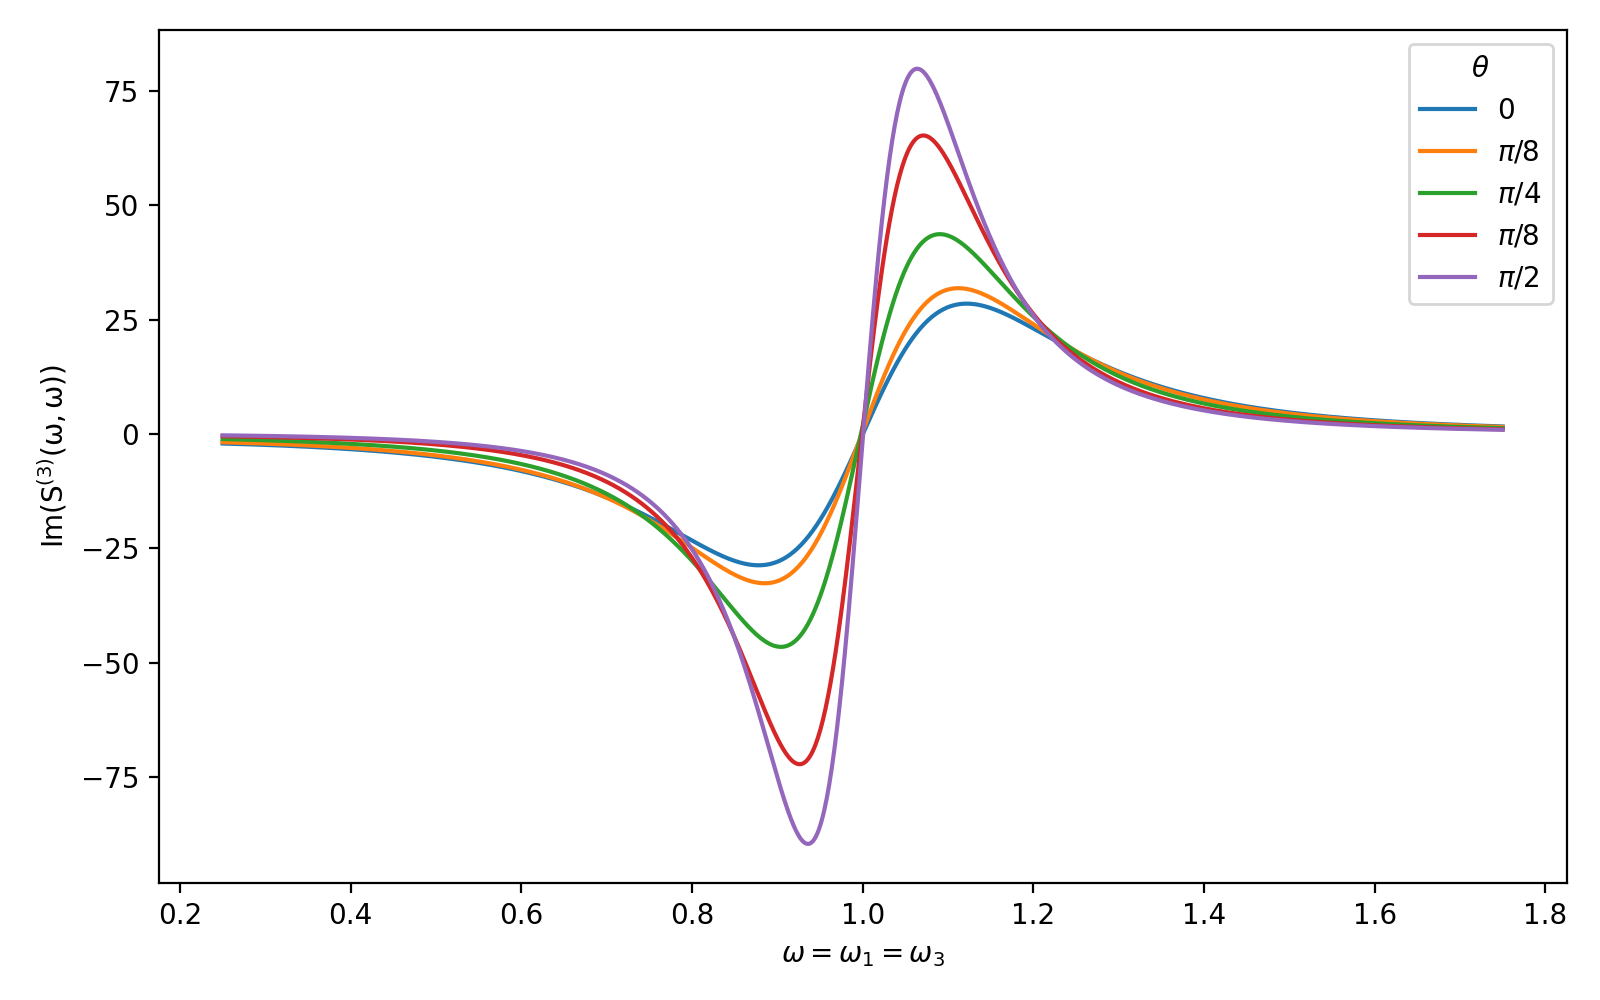
\includegraphics[width=\linewidth]{Figures/corrected_diag_theta_imag_2.png}
\end{minipage}
\caption{Real (left) and imaginary (right) components 
of the diagonal spectral response for increasing 
pointer-basis misalignment $\theta$. At $\theta = 0$, 
only dephasing contributions are present. For 
$\theta \neq 0$, basis misalignment mixes response 
pathways, producing continuous and structured 
deformations of the complex spectrum. These serve 
as benchmarks for the Duhamel reconstructions shown 
in Fig.~\ref{fig:TransportError}.}
\label{fig:DiagResponse}
\end{figure*}

\subsection{Spectroscopic Fingerprints of the Observable Bundle}
Figure~\ref{fig:DiagResponse} shows representative diagonal
spectral slices obtained from the full third-order response for
increasing values of the observational coordinate $\theta$. The
reported spectra include the complete third-order signal,
obtained by coherently summing all contributing Liouville
pathways, including both rephasing and non-rephasing sectors.
Within the canonical two-level chart these consist of the
ground-state bleach and excited-state absorption pathways
together with their corresponding rephasing and non-rephasing
contributions.

The Hamiltonian and optical transition operators are held fixed
throughout the calculation so that all observed spectral changes
originate solely from deformation of the Liouvillian geometry.
As the observational coordinate increases, transport between
Liouville pathways continuously redistributes both spectral
weight and phase, producing characteristic distortions in the
real and imaginary components of the nonlinear response.
The important observation is that these distortions are highly
structured and evolve continuously with $\theta$. The observable
coordinate therefore possesses a unique spectroscopic
fingerprint, establishing the forward mapping
\[
\theta
\longrightarrow
P^{(3)}(\omega_1,\omega_3),
\]
which forms the basis for geometric reconstruction.

\subsection{Accuracy of the Geometric Refinement}
The Duhamel expansion provides a systematic approximation to the
transport operator by successively refining the local
Liouvillian geometry. Figure~\ref{fig:TransportError} compares
the reconstruction error obtained from the zeroth-, first-, and
second-order transport expansions.

\begin{figure}
\centering
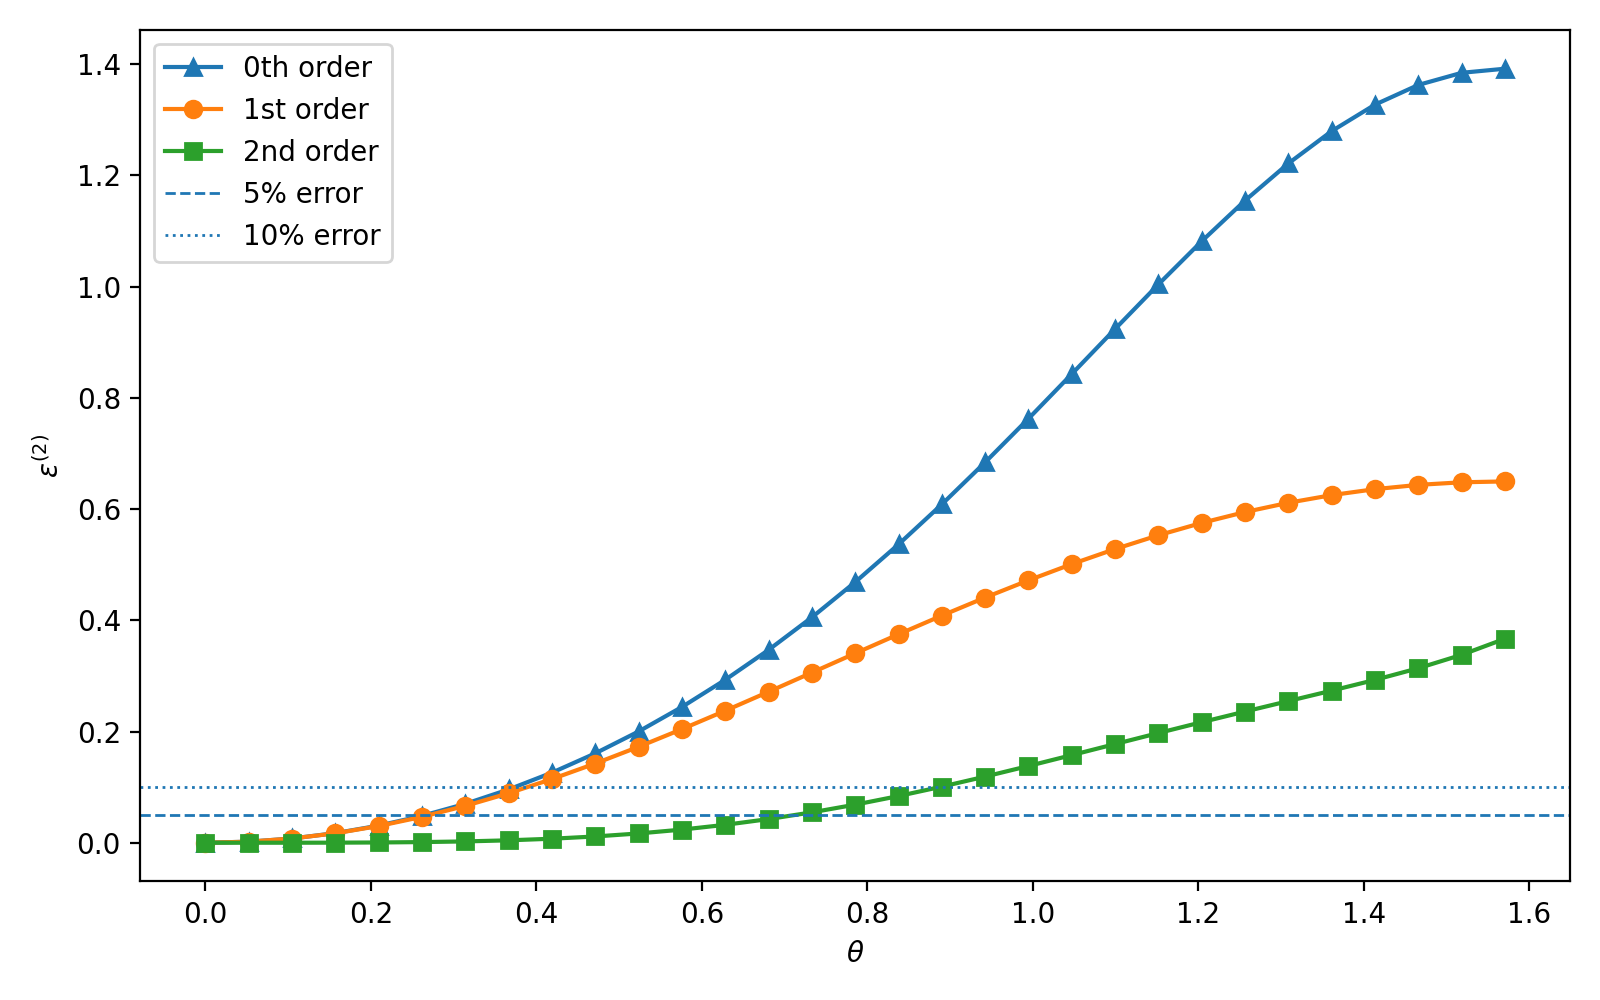
\includegraphics[width=0.75\linewidth]{Figures/duhamel_second_order_error_scaling_2.png}
\caption{Global reconstruction error $\epsilon^{(n)}$ 
for the first- and second-order Duhamel transport 
expansions as a function of pointer-basis misalignment 
$\theta$. The zeroth-order curve compares the 
$\theta = 0$ signal to the exact result at 
$\theta \neq 0$. The second-order approximation 
remains accurate throughout the full range of 
misalignment, including at $\theta = \pi/2$ where 
the observational and pointer bases are maximally 
misaligned.}
\label{fig:TransportError}
\end{figure}



Several features are noteworthy. First, the zeroth-order
approximation fails rapidly once the observational and pointer
bases become misaligned, illustrating that pathway transport is
an essential component of the nonlinear response. Second, the
first-order transport operator captures the dominant effects of
Liouville-space transport. Finally, inclusion of the second-order
terms reduces the reconstruction error by more than an order of
magnitude and remains quantitatively accurate over the entire
range of observational coordinates examined.

This behavior has a clear geometric interpretation. Although the
transport operator is constructed from a local expansion about
the reference geometry at $\theta=0$, the resulting coordinate
chart remains valid over a surprisingly large neighborhood of
the Liouvillian manifold. The canonical coordinate chart
therefore provides a robust local representation of the
observable bundle rather than merely an infinitesimal
approximation.

\begin{figure*}
\centering
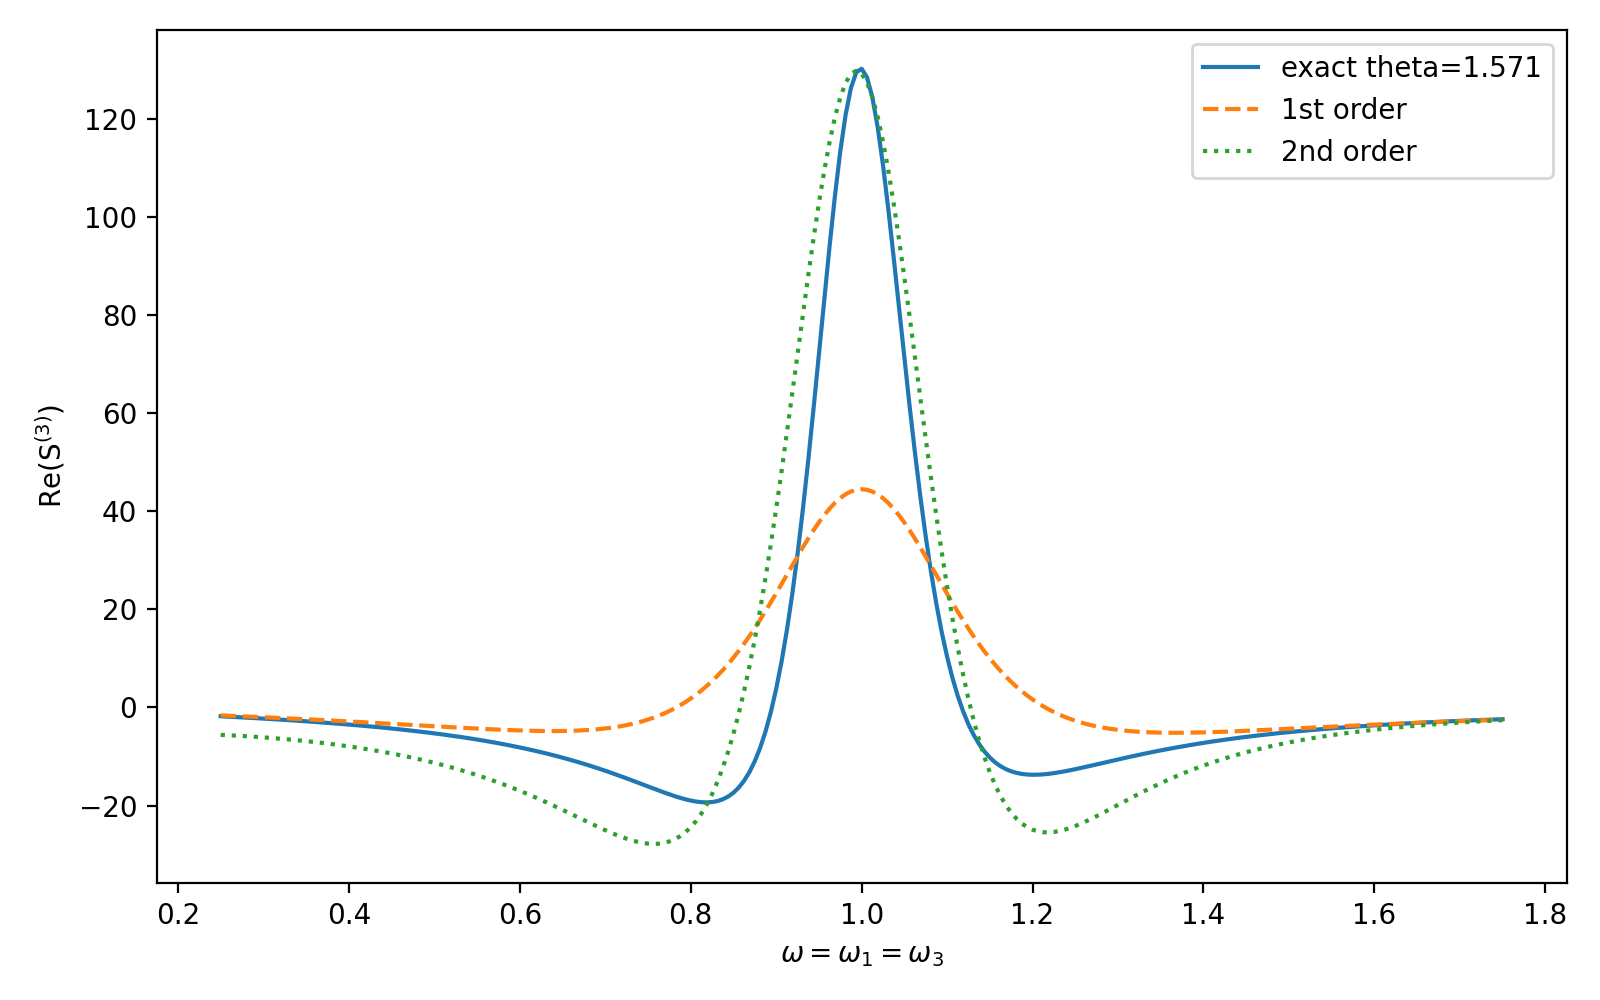
\includegraphics[width=0.48\linewidth]{Figures/duhamel_second_order_real_theta_1p571_2.png}
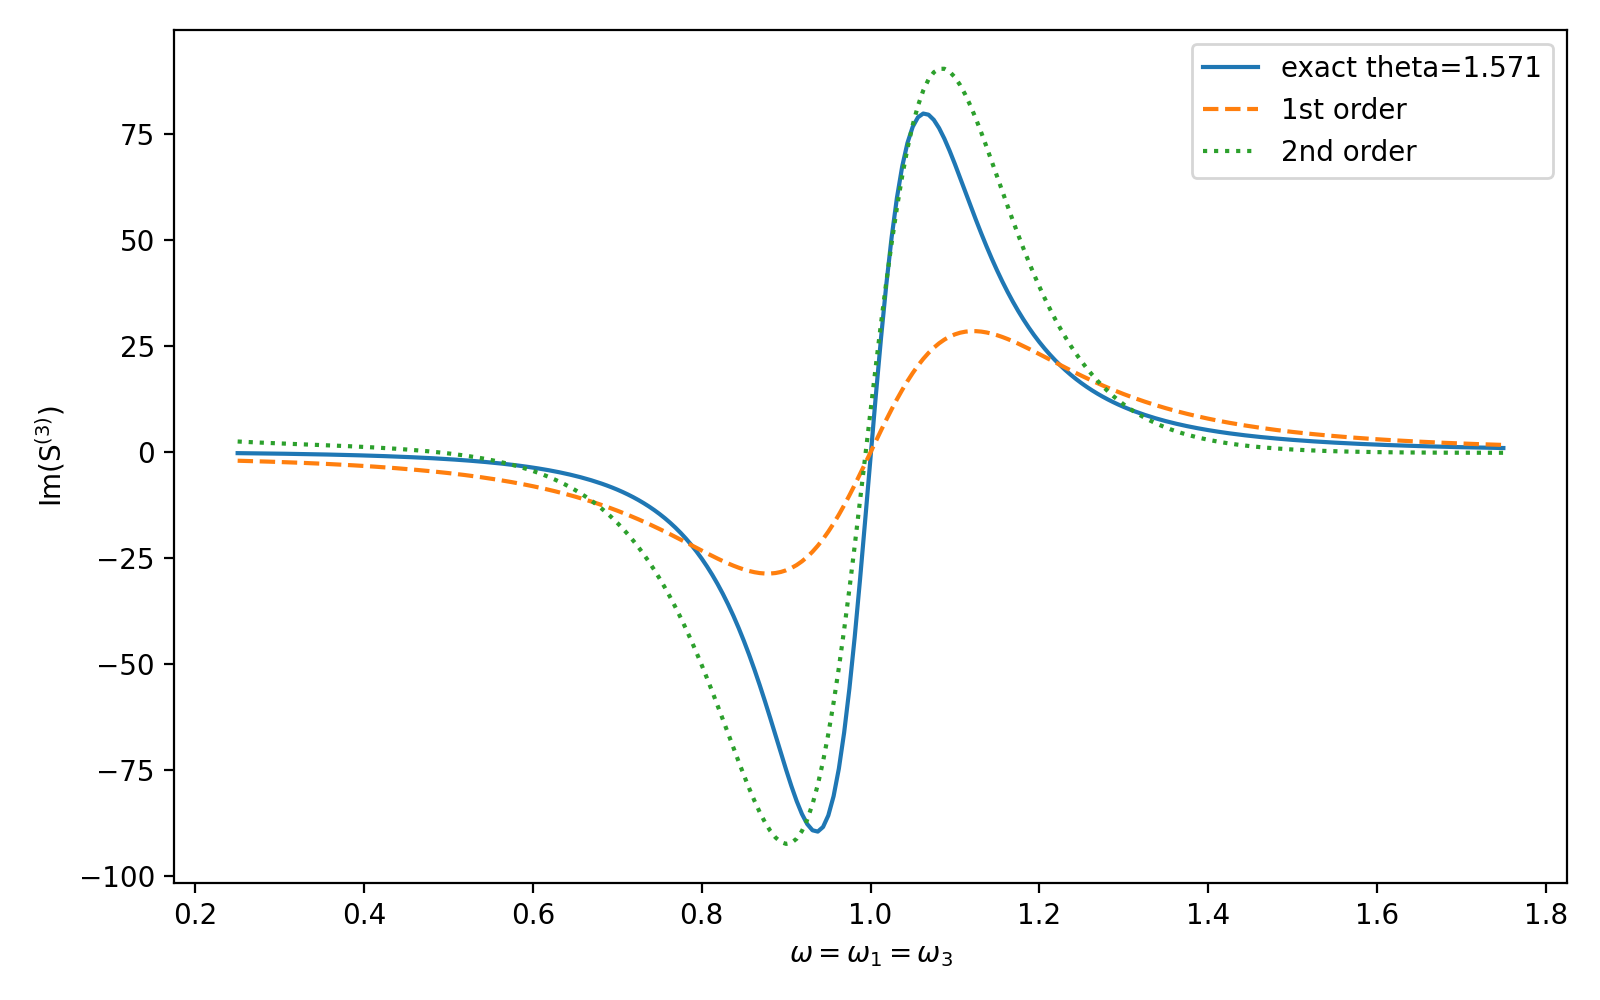
\includegraphics[width=0.48\linewidth]{Figures/duhamel_second_order_imag_theta_1p571_2.png}
\caption{Comparison between exact and reconstructed 
signals at maximal misalignment $\theta = \pi/2$. 
The second-order Duhamel reconstruction reproduces 
the exact response with high fidelity even in this 
strongly deformed regime.}
\label{fig:worst-case}
\end{figure*}


Figure~\ref{fig:worst-case} emphasizes this point by comparing
the exact and reconstructed spectra at
$\theta=\pi/2$, corresponding to maximal observational
deformation. Even in this strongly transported regime the
second-order transport operator accurately reproduces the full
nonlinear response, demonstrating that the dominant geometric
effects are captured by only a small number of transport
coefficients.

\subsection{From Spectral Analysis to Geometric Reconstruction}
The principal conclusion of these calculations is conceptual
rather than numerical. Conventional nonlinear spectroscopy seeks
a microscopic Hamiltonian and dissipative model capable of
reproducing the measured spectrum. Within the present framework,
the objective is instead to reconstruct the local geometry
responsible for the observed response.
The reconstruction proceeds through the hierarchy
\[
P^{(3)}
\Longrightarrow
\theta
\Longrightarrow
T_{ab}
\Longrightarrow
\Gamma_\mu
\Longrightarrow
\mathcal{K}_{\mu\nu},
\]
beginning with experimentally measured spectra and progressing
toward increasingly intrinsic geometric objects. The observable
coordinate determines the local transport operator acting on the
Liouville pathway basis. The transport operator, in turn,
provides direct information about the Liouvillian connection and
its associated curvature.

From this perspective, nonlinear spectroscopy is naturally
reinterpreted as an inverse geometric problem. The measured
spectrum is no longer regarded as the endpoint of the analysis,
but as the observable projection of an underlying response
geometry. Refining the microscopic model therefore becomes
equivalent to refining the local geometry itself, providing a
systematic route toward reconstructing increasingly accurate
Liouvillian manifolds directly from experiment.




\section*{Author contributions}
%We strongly encourage authors to include author contributions and recommend using \href{https://casrai.org/credit/}{CRediT} for standardised contribution descriptions. Please refer to our general \href{https://www.rsc.org/journals-books-databases/journal-authors-reviewers/author-responsibilities/}{author guidelines} for more information about authorship.

\section*{Conflicts of interest}
%In accordance with our policy on \href{https://www.rsc.org/journals-books-databases/journal-authors-reviewers/author-responsibilities/#code-of-conduct}{Conflicts of interest} please ensure that a conflicts of interest statement is included in your manuscript here.  Please note that this statement is required for all submitted manuscripts.  If no conflicts exist, please state that ``There are no conflicts to declare''.

\section*{Data availability}

%A data availability statement (DAS) is required to be submitted alongside all articles. Please read our \href{https://www.rsc.org/journals-books-databases/author-and-reviewer-hub/authors-information/prepare-and-format/data-sharing/#dataavailabilitystatements}{full guidance on data availability statements} for more details and examples of suitable statements you can use.

\section*{Acknowledgements}
The Acknowledgements come at the end of an article after Conflicts of interest and before the Notes and references.  Gimme some money. Gimme some money!

%%%END OF MAIN TEXT%%%

%The \balance command can be used to balance the columns on the final page if desired. It should be placed anywhere within the first column of the last page.

\balance

%If notes are included in your references you can change the title from 'References' to 'Notes and references' using the following command:
%\renewcommand\refname{Notes and references}

%%%REFERENCES%%%
\bibliography{bibliography/pccp_response_geometry_master} 
%You need to replace "rsc" on this line with the name of your .bib file
\bibliographystyle{rsc} %the RSC's .bst file

\end{document}
